\documentclass[a4paper,10.5pt]{ltjsarticle}
\usepackage{graphicx}
\usepackage{luatexja-fontspec}
\usepackage{caption}
\usepackage{amsmath,amssymb,bm,braket}
\usepackage{gnuplot-lua-tikz}
\usepackage[top=10truemm,bottom=15truemm,left=10truemm,right=10truemm]{geometry}
\usepackage{array}
\usepackage{upgreek}
\usepackage{fancyhdr}
\renewcommand{\refname}{}
\usepackage{listings,jvlisting}
\usepackage{tikz}
\usetikzlibrary{external}
\tikzexternalize
\lstset{
  basicstyle={\ttfamily},
  identifierstyle={\small},
  commentstyle={\smallitshape},
  keywordstyle={\small\bfseries},
  ndkeywordstyle={\small},
  stringstyle={\small\ttfamily},
  frame={tb},
  breaklines=true,
  columns=[l]{fullflexible},
  numbers=left,
  xrightmargin=0pt,
  xleftmargin=3pt,
  numberstyle={\scriptsize},
  stepnumber=1,
  numbersep=1pt,
  lineskip=-0.5ex
}
\captionsetup[figure]{format=plain, labelformat=simple, labelsep=quad,labelfont=bf}
\captionsetup[table]{format=plain, labelformat=simple, labelsep=quad,labelfont=bf}
\parindent = 0pt
\setmainjfont[BoldFont=HiraMinProN-W6]{HiraMinPro-W3}
%[BoldFont=HGSMinchoE]{MSMincho}[BoldFont=HiraMinProN-W6]{HiraMinPro-W3}
\begin{document}
\centerline{\HUGE \bfseries 物理情報工学CD実験 報告書}
\centerline{ }
\rightline{\vspace{-3mm} \Large 2023年度   }
\begin{table}[h]
  \newcolumntype{I}{!{\vrule width 1.5pt}}
  \newcolumntype{i}{!{\vrule width 0.8pt}}
  \arrayrulewidth=0.8pt
  \renewcommand{\arraystretch}{1.5}
  \newcommand{\bhline}[1]{\noalign{\hrule height #1}}
  \huge
  \centering
  \begin{tabular}{Iwc{6cm}Iwc{2cm}iciwc{5cm}I}
    \bhline{1.5pt}
    実験テーマ&\multicolumn{3}{cI}{B5 光ファイバー}\\
    \hline
    担当教員名&\multicolumn{3}{cI}{一ノ瀬TA\&市塚TA}\\
    \hline
    実験整理番号&80&実験者氏名&平井 優我\\
    \hline
    共同実験者氏名&\multicolumn{3}{cI}{肥田\ 侑真、日野\ 正一}\\
    \hline
    曜日組&木&実験日&12月7日\\
    \hline
    実験回&7&報告書提出日&12月13日\\
    \bhline{1.5pt}
  \end{tabular}
\end{table}
\clearpage
%1-2-------------------------------------------------------------------------
\hspace{-2pt}{\Large \bfseries 1.目的}\\
 本実験では、はじめに高速通信線路に光ファイバが必要となる理由につ
いて考える。さらに,光ファイバの伝送速度を支配する分散要因について理解し、高
速通信を実現するための、光ファイバの構造上の工夫を学ぶ。また、実際に様々な光
ファイバに触れ、光結合、伝送損失、伝送帯域測定などを通して、光ファイバの光学
特性について学ぶ。\\
\\
\hspace{-2pt}{\Large \bfseries 2.結果}\\
{\large \bfseries 2.1 光ファイバへの光結合実験}\\
 表\ref{efficiency}に光ファイバから出てきた光強度と結合効率を示す。ただし、レーザーの発光強度は$7.2\ \mathrm{mW}$、波長は$633\ \mathrm{nm}$であった。
\begin{table}[h]
  \newcolumntype{I}{!{\vrule width 1.5pt}}
  \newcolumntype{i}{!{\vrule width 0.5pt}}
  \arrayrulewidth=0.8pt
  \renewcommand{\arraystretch}{1.5}
  \newcommand{\bhline}[1]{\noalign{\hrule height #1}}
  \centering
  \caption{光ファイバの結合効率}
  \label{efficiency}
  \begin{tabular}{IcicccI}
    \bhline{1.5pt}
    光ファイバの種類&
    \begin{tabular}{c}
      $10\ \mathrm{\upmu m}$径の\\[-10pt]シングルモードファイバ
    \end{tabular}&
    \begin{tabular}{c}
      200$\ \mathrm{\upmu m}$径の\\[-10pt]マルチモードファイバ
    \end{tabular}&
    \begin{tabular}{c}
      $50\ \mathrm{\upmu m}$径の\\[-10pt]マルチモードファイバ
    \end{tabular}\\
    \hline
    光ファイバの長さ$\ /\ \mathrm{m}$&1&1&1\\
    ケーブルの色&黄色&橙色&水色\\
    最大の光強度$\ /\ \mathrm{\upmu W}$&2.577&650.5&41.94\\
    \begin{tabular}{c}
      20$\ \mathrm{\upmu m}$位置をずらした\\[-10pt]
      ときの光強度$\ /\ \mathrm{\upmu W}$\\
    \end{tabular}
    &2.499&642.2&43.12\\
    結合効率$\mathrm{\ /\ \%}$&0.03579&8.919&0.5825\\
    \bhline{1.5pt}
  \end{tabular}
\end{table}\\
表\ref{efficiency}から、測定の位置を$20\ \mathrm{\upmu m}$ずらしても光強度はあまり変わらなかった。また、光ファイバのコアの面積と結合効率には正の相関がみられた。\\
\\
{\large \bfseries 2.2 光ファイバの伝送損失測定}\\
 表\ref{lengthefficiency}に光ファイバーの長さを変えたときの出射光強度を示す。そして、そのグラフを図\ref{loss}に示す。ただし、グラフの直線は回帰直線を表す。
\begin{table}[h]
  \newcolumntype{I}{!{\vrule width 1.5pt}}
  \newcolumntype{i}{!{\vrule width 0.5pt}}
  \arrayrulewidth=0.8pt
  \renewcommand{\arraystretch}{1.5}
  \newcommand{\bhline}[1]{\noalign{\hrule height #1}}
  \centering
  \caption{光ファイバの出射光強度}
  \label{lengthefficiency}
  \begin{tabular}{IcicI}
    \bhline{1.5pt}
    ファイバ長$\ /\ \mathrm{m}$&光強度$/\ \mathrm{dBm}$\\
    \hline
    161&$-13.7$\\
    61&$-10.2$\\
    11&$-7.43$\\
    1&$-6.48$\\
    \bhline{1.5pt}
  \end{tabular}
\end{table}
\clearpage
\begin{figure}[h]
  \centering
  \scalebox{0.45}[0.45]{
\begin{tikzpicture}[gnuplot]
%% generated with GNUPLOT 5.4p10 (Lua 5.4; terminal rev. Jun 2020, script rev. 118)
%% Sun Nov 12 18:33:30 2023
\path (0.000,0.000) rectangle (12.500,8.750);
\gpcolor{color=gp lt color border}
\gpsetlinetype{gp lt border}
\gpsetdashtype{gp dt solid}
\gpsetlinewidth{1.00}
\draw[gp path] (0.018,0.031)--(0.198,0.031);
\draw[gp path] (12.480,0.031)--(12.300,0.031);
\node[gp node right] at (-0.166,0.031) {$15$};
\draw[gp path] (0.018,1.479)--(0.198,1.479);
\draw[gp path] (12.480,1.479)--(12.300,1.479);
\node[gp node right] at (-0.166,1.479) {$20$};
\draw[gp path] (0.018,2.927)--(0.198,2.927);
\draw[gp path] (12.480,2.927)--(12.300,2.927);
\node[gp node right] at (-0.166,2.927) {$25$};
\draw[gp path] (0.018,4.375)--(0.198,4.375);
\draw[gp path] (12.480,4.375)--(12.300,4.375);
\node[gp node right] at (-0.166,4.375) {$30$};
\draw[gp path] (0.018,5.822)--(0.198,5.822);
\draw[gp path] (12.480,5.822)--(12.300,5.822);
\node[gp node right] at (-0.166,5.822) {$35$};
\draw[gp path] (0.018,7.270)--(0.198,7.270);
\draw[gp path] (12.480,7.270)--(12.300,7.270);
\node[gp node right] at (-0.166,7.270) {$40$};
\draw[gp path] (0.018,8.718)--(0.198,8.718);
\draw[gp path] (12.480,8.718)--(12.300,8.718);
\node[gp node right] at (-0.166,8.718) {$45$};
\draw[gp path] (0.018,0.031)--(0.018,0.211);
\draw[gp path] (0.018,8.718)--(0.018,8.538);
\node[gp node center] at (0.018,-0.277) {$0$};
\draw[gp path] (1.935,0.031)--(1.935,0.211);
\draw[gp path] (1.935,8.718)--(1.935,8.538);
\node[gp node center] at (1.935,-0.277) {$0.2$};
\draw[gp path] (3.852,0.031)--(3.852,0.211);
\draw[gp path] (3.852,8.718)--(3.852,8.538);
\node[gp node center] at (3.852,-0.277) {$0.4$};
\draw[gp path] (5.770,0.031)--(5.770,0.211);
\draw[gp path] (5.770,8.718)--(5.770,8.538);
\node[gp node center] at (5.770,-0.277) {$0.6$};
\draw[gp path] (7.687,0.031)--(7.687,0.211);
\draw[gp path] (7.687,8.718)--(7.687,8.538);
\node[gp node center] at (7.687,-0.277) {$0.8$};
\draw[gp path] (9.604,0.031)--(9.604,0.211);
\draw[gp path] (9.604,8.718)--(9.604,8.538);
\node[gp node center] at (9.604,-0.277) {$1$};
\draw[gp path] (11.521,0.031)--(11.521,0.211);
\draw[gp path] (11.521,8.718)--(11.521,8.538);
\node[gp node center] at (11.521,-0.277) {$1.2$};
\draw[gp path] (0.018,8.718)--(0.018,0.031)--(12.480,0.031)--(12.480,8.718)--cycle;
\node[gp node center,rotate=-270] at (-0.826,4.374) {$J$};
\node[gp node center] at (6.249,-0.738) {$F^*$};
\gpcolor{rgb color={0.000,0.000,0.000}}
\gpsetlinewidth{5.00}
\draw[gp path] (0.977,8.142)--(1.935,3.417)--(2.894,1.542)--(3.852,0.700)--(4.811,0.321)%
  --(5.770,0.196)--(5.943,0.194)--(6.728,0.244)--(7.687,0.429)--(8.646,0.742)--(9.604,1.189)%
  --(10.563,1.795)--(11.521,2.601);
\gpsetpointsize{3.20}
\gp3point{gp mark 7}{}{(0.977,8.142)}
\gp3point{gp mark 7}{}{(1.935,3.417)}
\gp3point{gp mark 7}{}{(2.894,1.542)}
\gp3point{gp mark 7}{}{(3.852,0.700)}
\gp3point{gp mark 7}{}{(4.811,0.321)}
\gp3point{gp mark 7}{}{(5.770,0.196)}
\gp3point{gp mark 7}{}{(5.943,0.194)}
\gp3point{gp mark 7}{}{(6.728,0.244)}
\gp3point{gp mark 7}{}{(7.687,0.429)}
\gp3point{gp mark 7}{}{(8.646,0.742)}
\gp3point{gp mark 7}{}{(9.604,1.189)}
\gp3point{gp mark 7}{}{(10.563,1.795)}
\gp3point{gp mark 7}{}{(11.521,2.601)}
\gpcolor{color=gp lt color border}
\gpsetlinewidth{1.00}
\draw[gp path] (0.018,8.718)--(0.018,0.031)--(12.480,0.031)--(12.480,8.718)--cycle;
%% coordinates of the plot area
\gpdefrectangularnode{gp plot 1}{\pgfpoint{0.018cm}{0.031cm}}{\pgfpoint{12.480cm}{8.718cm}}
\end{tikzpicture}
}

  \vspace{-30pt}\caption{ファイバ長と光強度の関係}
  \label{loss}
\end{figure}
グラフから回帰直線の傾きは$-0.044\ \mathrm{dBm/m}$であるから、伝送損失は$44\ \mathrm{dB/km}$と求まる。\\
\\
{\large \bfseries 2.3 光ファイバの屈折率分布測定}\\
 図\ref{GI}、図\ref{SI}に実験によって得られた光強度分布の写真とグラフを示す。
\begin{figure}[h]
  \centering
  \begin{minipage}[h]{0.48\linewidth}
    \includegraphics[scale=0.20]{figure1.eps}
    \vspace{25pt}\caption*{(a)}
    \label{}
  \end{minipage}
  \vspace{30pt}\begin{minipage}[h]{0.38\linewidth}
    \scalebox{0.5}[0.5]{
\begin{tikzpicture}[gnuplot]
%% generated with GNUPLOT 5.4p10 (Lua 5.4; terminal rev. Jun 2020, script rev. 118)
%% Sat Dec  9 17:21:03 2023
\path (0.000,0.000) rectangle (12.500,8.750);
\gpcolor{color=gp lt color border}
\gpsetlinetype{gp lt border}
\gpsetdashtype{gp dt solid}
\gpsetlinewidth{1.00}
\draw[gp path] (0.018,0.031)--(0.198,0.031);
\draw[gp path] (12.480,0.031)--(12.300,0.031);
\node[gp node right] at (-0.166,0.031) {$0$};
\draw[gp path] (0.018,0.900)--(0.198,0.900);
\draw[gp path] (12.480,0.900)--(12.300,0.900);
\node[gp node right] at (-0.166,0.900) {$0.1$};
\draw[gp path] (0.018,1.768)--(0.198,1.768);
\draw[gp path] (12.480,1.768)--(12.300,1.768);
\node[gp node right] at (-0.166,1.768) {$0.2$};
\draw[gp path] (0.018,2.637)--(0.198,2.637);
\draw[gp path] (12.480,2.637)--(12.300,2.637);
\node[gp node right] at (-0.166,2.637) {$0.3$};
\draw[gp path] (0.018,3.506)--(0.198,3.506);
\draw[gp path] (12.480,3.506)--(12.300,3.506);
\node[gp node right] at (-0.166,3.506) {$0.4$};
\draw[gp path] (0.018,4.375)--(0.198,4.375);
\draw[gp path] (12.480,4.375)--(12.300,4.375);
\node[gp node right] at (-0.166,4.375) {$0.5$};
\draw[gp path] (0.018,5.243)--(0.198,5.243);
\draw[gp path] (12.480,5.243)--(12.300,5.243);
\node[gp node right] at (-0.166,5.243) {$0.6$};
\draw[gp path] (0.018,6.112)--(0.198,6.112);
\draw[gp path] (12.480,6.112)--(12.300,6.112);
\node[gp node right] at (-0.166,6.112) {$0.7$};
\draw[gp path] (0.018,6.981)--(0.198,6.981);
\draw[gp path] (12.480,6.981)--(12.300,6.981);
\node[gp node right] at (-0.166,6.981) {$0.8$};
\draw[gp path] (0.018,7.849)--(0.198,7.849);
\draw[gp path] (12.480,7.849)--(12.300,7.849);
\node[gp node right] at (-0.166,7.849) {$0.9$};
\draw[gp path] (0.018,8.718)--(0.198,8.718);
\draw[gp path] (12.480,8.718)--(12.300,8.718);
\node[gp node right] at (-0.166,8.718) {$1$};
\draw[gp path] (0.018,0.031)--(0.018,0.211);
\draw[gp path] (0.018,8.718)--(0.018,8.538);
\node[gp node center] at (0.018,-0.277) {$1200$};
\draw[gp path] (1.576,0.031)--(1.576,0.211);
\draw[gp path] (1.576,8.718)--(1.576,8.538);
\node[gp node center] at (1.576,-0.277) {$1250$};
\draw[gp path] (3.134,0.031)--(3.134,0.211);
\draw[gp path] (3.134,8.718)--(3.134,8.538);
\node[gp node center] at (3.134,-0.277) {$1300$};
\draw[gp path] (4.691,0.031)--(4.691,0.211);
\draw[gp path] (4.691,8.718)--(4.691,8.538);
\node[gp node center] at (4.691,-0.277) {$1350$};
\draw[gp path] (6.249,0.031)--(6.249,0.211);
\draw[gp path] (6.249,8.718)--(6.249,8.538);
\node[gp node center] at (6.249,-0.277) {$1400$};
\draw[gp path] (7.807,0.031)--(7.807,0.211);
\draw[gp path] (7.807,8.718)--(7.807,8.538);
\node[gp node center] at (7.807,-0.277) {$1450$};
\draw[gp path] (9.365,0.031)--(9.365,0.211);
\draw[gp path] (9.365,8.718)--(9.365,8.538);
\node[gp node center] at (9.365,-0.277) {$1500$};
\draw[gp path] (10.922,0.031)--(10.922,0.211);
\draw[gp path] (10.922,8.718)--(10.922,8.538);
\node[gp node center] at (10.922,-0.277) {$1550$};
\draw[gp path] (12.480,0.031)--(12.480,0.211);
\draw[gp path] (12.480,8.718)--(12.480,8.538);
\node[gp node center] at (12.480,-0.277) {$1600$};
\draw[gp path] (0.018,8.718)--(0.018,0.031)--(12.480,0.031)--(12.480,8.718)--cycle;
\node[gp node center,rotate=-270,font={\fontsize{17.0pt}{20.4pt}\selectfont}] at (-1.286,4.374) {光強度比$P(r)/P(0)$};
\node[gp node center,font={\fontsize{17.0pt}{20.4pt}\selectfont}] at (6.249,-1.046) {距離$\ /\ \mathrm{\upmu m}$};
\gpcolor{rgb color={0.000,0.000,0.000}}
\draw[gp path] (0.018,0.207)--(0.064,0.221)--(0.110,0.218)--(0.156,0.205)--(0.202,0.205)%
  --(0.248,0.183)--(0.294,0.196)--(0.340,0.210)--(0.386,0.207)--(0.431,0.176)--(0.477,0.212)%
  --(0.523,0.212)--(0.569,0.198)--(0.615,0.210)--(0.661,0.198)--(0.707,0.207)--(0.753,0.203)%
  --(0.799,0.225)--(0.845,0.198)--(0.891,0.223)--(0.937,0.203)--(0.983,0.218)--(1.029,0.205)%
  --(1.075,0.205)--(1.121,0.216)--(1.167,0.203)--(1.213,0.203)--(1.259,0.196)--(1.305,0.212)%
  --(1.351,0.189)--(1.397,0.205)--(1.443,0.216)--(1.489,0.214)--(1.535,0.205)--(1.581,0.207)%
  --(1.627,0.207)--(1.673,0.201)--(1.719,0.221)--(1.765,0.216)--(1.811,0.207)--(1.857,0.207)%
  --(1.903,0.198)--(1.949,0.205)--(1.995,0.205)--(2.041,0.212)--(2.087,0.221)--(2.133,0.210)%
  --(2.179,0.218)--(2.225,0.218)--(2.271,0.225)--(2.317,0.214)--(2.363,0.212)--(2.409,0.205)%
  --(2.455,0.221)--(2.501,0.223)--(2.547,0.227)--(2.593,0.203)--(2.639,0.194)--(2.685,0.210)%
  --(2.731,0.214)--(2.777,0.205)--(2.823,0.194)--(2.869,0.210)--(2.915,0.194)--(2.961,0.212)%
  --(3.007,0.205)--(3.053,0.225)--(3.099,0.223)--(3.145,0.205)--(3.191,0.221)--(3.237,0.216)%
  --(3.283,0.216)--(3.329,0.214)--(3.375,0.212)--(3.420,0.212)--(3.466,0.212)--(3.512,0.212)%
  --(3.558,0.227)--(3.604,0.203)--(3.650,0.207)--(3.696,0.223)--(3.742,0.194)--(3.788,0.212)%
  --(3.834,0.218)--(3.880,0.225)--(3.926,0.207)--(3.972,0.210)--(4.018,0.185)--(4.064,0.223)%
  --(4.110,0.205)--(4.156,0.207)--(4.202,0.218)--(4.248,0.198)--(4.294,0.225)--(4.340,0.216)%
  --(4.386,0.203)--(4.432,0.192)--(4.478,0.187)--(4.524,0.225)--(4.570,0.189)--(4.616,0.212)%
  --(4.662,0.221)--(4.708,0.221)--(4.754,0.203)--(4.800,0.234)--(4.846,0.214)--(4.892,0.223)%
  --(4.938,0.203)--(4.984,0.232)--(5.030,0.210)--(5.076,0.210)--(5.122,0.216)--(5.168,0.203)%
  --(5.214,0.236)--(5.260,0.223)--(5.306,0.227)--(5.352,0.207)--(5.398,0.243)--(5.444,0.225)%
  --(5.490,0.194)--(5.536,0.218)--(5.582,0.245)--(5.628,0.225)--(5.674,0.225)--(5.720,0.214)%
  --(5.766,0.250)--(5.812,0.223)--(5.858,0.261)--(5.904,0.256)--(5.950,0.256)--(5.996,0.301)%
  --(6.042,0.361)--(6.088,0.426)--(6.134,0.553)--(6.180,0.823)--(6.226,1.173)--(6.272,1.707)%
  --(6.318,2.633)--(6.364,3.720)--(6.410,4.612)--(6.455,5.458)--(6.501,5.969)--(6.547,6.634)%
  --(6.593,7.011)--(6.639,7.578)--(6.685,7.774)--(6.731,8.107)--(6.777,8.205)--(6.823,8.339)%
  --(6.869,8.515)--(6.915,8.497)--(6.961,8.444)--(7.007,8.718)--(7.053,8.696)--(7.099,8.611)%
  --(7.145,8.564)--(7.191,8.535)--(7.237,8.479)--(7.283,8.272)--(7.329,7.850)--(7.375,7.522)%
  --(7.421,6.899)--(7.467,6.092)--(7.513,5.137)--(7.559,4.146)--(7.605,2.970)--(7.651,2.124)%
  --(7.697,1.470)--(7.743,1.115)--(7.789,0.841)--(7.835,0.618)--(7.881,0.500)--(7.927,0.386)%
  --(7.973,0.343)--(8.019,0.294)--(8.065,0.281)--(8.111,0.245)--(8.157,0.241)--(8.203,0.203)%
  --(8.249,0.245)--(8.295,0.256)--(8.341,0.205)--(8.387,0.210)--(8.433,0.221)--(8.479,0.230)%
  --(8.525,0.218)--(8.571,0.201)--(8.617,0.216)--(8.663,0.221)--(8.709,0.183)--(8.755,0.218)%
  --(8.801,0.201)--(8.847,0.218)--(8.893,0.212)--(8.939,0.205)--(8.985,0.201)--(9.031,0.218)%
  --(9.077,0.227)--(9.123,0.223)--(9.169,0.218)--(9.215,0.214)--(9.261,0.223)--(9.307,0.198)%
  --(9.353,0.221)--(9.399,0.201)--(9.445,0.216)--(9.490,0.236)--(9.536,0.216)--(9.582,0.203)%
  --(9.628,0.221)--(9.674,0.196)--(9.720,0.207)--(9.766,0.212)--(9.812,0.207)--(9.858,0.196)%
  --(9.904,0.212)--(9.950,0.218)--(9.996,0.198)--(10.042,0.225)--(10.088,0.205)--(10.134,0.216)%
  --(10.180,0.207)--(10.226,0.225)--(10.272,0.212)--(10.318,0.203)--(10.364,0.201)--(10.410,0.214)%
  --(10.456,0.198)--(10.502,0.214)--(10.548,0.205)--(10.594,0.210)--(10.640,0.192)--(10.686,0.225)%
  --(10.732,0.210)--(10.778,0.216)--(10.824,0.210)--(10.870,0.214)--(10.916,0.201)--(10.962,0.207)%
  --(11.008,0.216)--(11.054,0.205)--(11.100,0.212)--(11.146,0.218)--(11.192,0.218)--(11.238,0.210)%
  --(11.284,0.205)--(11.330,0.212)--(11.376,0.198)--(11.422,0.214)--(11.468,0.189)--(11.514,0.214)%
  --(11.560,0.225)--(11.606,0.210)--(11.652,0.225)--(11.698,0.216)--(11.744,0.214)--(11.790,0.214)%
  --(11.836,0.192)--(11.882,0.230)--(11.928,0.205)--(11.974,0.207)--(12.020,0.214)--(12.066,0.218)%
  --(12.112,0.198)--(12.158,0.221)--(12.204,0.201)--(12.250,0.221)--(12.296,0.214)--(12.342,0.210)%
  --(12.388,0.196)--(12.434,0.205)--(12.480,0.207);
\gpsetpointsize{1.20}
\gp3point{gp mark 7}{}{(0.064,0.221)}
\gp3point{gp mark 7}{}{(0.110,0.218)}
\gp3point{gp mark 7}{}{(0.156,0.205)}
\gp3point{gp mark 7}{}{(0.202,0.205)}
\gp3point{gp mark 7}{}{(0.248,0.183)}
\gp3point{gp mark 7}{}{(0.294,0.196)}
\gp3point{gp mark 7}{}{(0.340,0.210)}
\gp3point{gp mark 7}{}{(0.386,0.207)}
\gp3point{gp mark 7}{}{(0.431,0.176)}
\gp3point{gp mark 7}{}{(0.477,0.212)}
\gp3point{gp mark 7}{}{(0.523,0.212)}
\gp3point{gp mark 7}{}{(0.569,0.198)}
\gp3point{gp mark 7}{}{(0.615,0.210)}
\gp3point{gp mark 7}{}{(0.661,0.198)}
\gp3point{gp mark 7}{}{(0.707,0.207)}
\gp3point{gp mark 7}{}{(0.753,0.203)}
\gp3point{gp mark 7}{}{(0.799,0.225)}
\gp3point{gp mark 7}{}{(0.845,0.198)}
\gp3point{gp mark 7}{}{(0.891,0.223)}
\gp3point{gp mark 7}{}{(0.937,0.203)}
\gp3point{gp mark 7}{}{(0.983,0.218)}
\gp3point{gp mark 7}{}{(1.029,0.205)}
\gp3point{gp mark 7}{}{(1.075,0.205)}
\gp3point{gp mark 7}{}{(1.121,0.216)}
\gp3point{gp mark 7}{}{(1.167,0.203)}
\gp3point{gp mark 7}{}{(1.213,0.203)}
\gp3point{gp mark 7}{}{(1.259,0.196)}
\gp3point{gp mark 7}{}{(1.305,0.212)}
\gp3point{gp mark 7}{}{(1.351,0.189)}
\gp3point{gp mark 7}{}{(1.397,0.205)}
\gp3point{gp mark 7}{}{(1.443,0.216)}
\gp3point{gp mark 7}{}{(1.489,0.214)}
\gp3point{gp mark 7}{}{(1.535,0.205)}
\gp3point{gp mark 7}{}{(1.581,0.207)}
\gp3point{gp mark 7}{}{(1.627,0.207)}
\gp3point{gp mark 7}{}{(1.673,0.201)}
\gp3point{gp mark 7}{}{(1.719,0.221)}
\gp3point{gp mark 7}{}{(1.765,0.216)}
\gp3point{gp mark 7}{}{(1.811,0.207)}
\gp3point{gp mark 7}{}{(1.857,0.207)}
\gp3point{gp mark 7}{}{(1.903,0.198)}
\gp3point{gp mark 7}{}{(1.949,0.205)}
\gp3point{gp mark 7}{}{(1.995,0.205)}
\gp3point{gp mark 7}{}{(2.041,0.212)}
\gp3point{gp mark 7}{}{(2.087,0.221)}
\gp3point{gp mark 7}{}{(2.133,0.210)}
\gp3point{gp mark 7}{}{(2.179,0.218)}
\gp3point{gp mark 7}{}{(2.225,0.218)}
\gp3point{gp mark 7}{}{(2.271,0.225)}
\gp3point{gp mark 7}{}{(2.317,0.214)}
\gp3point{gp mark 7}{}{(2.363,0.212)}
\gp3point{gp mark 7}{}{(2.409,0.205)}
\gp3point{gp mark 7}{}{(2.455,0.221)}
\gp3point{gp mark 7}{}{(2.501,0.223)}
\gp3point{gp mark 7}{}{(2.547,0.227)}
\gp3point{gp mark 7}{}{(2.593,0.203)}
\gp3point{gp mark 7}{}{(2.639,0.194)}
\gp3point{gp mark 7}{}{(2.685,0.210)}
\gp3point{gp mark 7}{}{(2.731,0.214)}
\gp3point{gp mark 7}{}{(2.777,0.205)}
\gp3point{gp mark 7}{}{(2.823,0.194)}
\gp3point{gp mark 7}{}{(2.869,0.210)}
\gp3point{gp mark 7}{}{(2.915,0.194)}
\gp3point{gp mark 7}{}{(2.961,0.212)}
\gp3point{gp mark 7}{}{(3.007,0.205)}
\gp3point{gp mark 7}{}{(3.053,0.225)}
\gp3point{gp mark 7}{}{(3.099,0.223)}
\gp3point{gp mark 7}{}{(3.145,0.205)}
\gp3point{gp mark 7}{}{(3.191,0.221)}
\gp3point{gp mark 7}{}{(3.237,0.216)}
\gp3point{gp mark 7}{}{(3.283,0.216)}
\gp3point{gp mark 7}{}{(3.329,0.214)}
\gp3point{gp mark 7}{}{(3.375,0.212)}
\gp3point{gp mark 7}{}{(3.420,0.212)}
\gp3point{gp mark 7}{}{(3.466,0.212)}
\gp3point{gp mark 7}{}{(3.512,0.212)}
\gp3point{gp mark 7}{}{(3.558,0.227)}
\gp3point{gp mark 7}{}{(3.604,0.203)}
\gp3point{gp mark 7}{}{(3.650,0.207)}
\gp3point{gp mark 7}{}{(3.696,0.223)}
\gp3point{gp mark 7}{}{(3.742,0.194)}
\gp3point{gp mark 7}{}{(3.788,0.212)}
\gp3point{gp mark 7}{}{(3.834,0.218)}
\gp3point{gp mark 7}{}{(3.880,0.225)}
\gp3point{gp mark 7}{}{(3.926,0.207)}
\gp3point{gp mark 7}{}{(3.972,0.210)}
\gp3point{gp mark 7}{}{(4.018,0.185)}
\gp3point{gp mark 7}{}{(4.064,0.223)}
\gp3point{gp mark 7}{}{(4.110,0.205)}
\gp3point{gp mark 7}{}{(4.156,0.207)}
\gp3point{gp mark 7}{}{(4.202,0.218)}
\gp3point{gp mark 7}{}{(4.248,0.198)}
\gp3point{gp mark 7}{}{(4.294,0.225)}
\gp3point{gp mark 7}{}{(4.340,0.216)}
\gp3point{gp mark 7}{}{(4.386,0.203)}
\gp3point{gp mark 7}{}{(4.432,0.192)}
\gp3point{gp mark 7}{}{(4.478,0.187)}
\gp3point{gp mark 7}{}{(4.524,0.225)}
\gp3point{gp mark 7}{}{(4.570,0.189)}
\gp3point{gp mark 7}{}{(4.616,0.212)}
\gp3point{gp mark 7}{}{(4.662,0.221)}
\gp3point{gp mark 7}{}{(4.708,0.221)}
\gp3point{gp mark 7}{}{(4.754,0.203)}
\gp3point{gp mark 7}{}{(4.800,0.234)}
\gp3point{gp mark 7}{}{(4.846,0.214)}
\gp3point{gp mark 7}{}{(4.892,0.223)}
\gp3point{gp mark 7}{}{(4.938,0.203)}
\gp3point{gp mark 7}{}{(4.984,0.232)}
\gp3point{gp mark 7}{}{(5.030,0.210)}
\gp3point{gp mark 7}{}{(5.076,0.210)}
\gp3point{gp mark 7}{}{(5.122,0.216)}
\gp3point{gp mark 7}{}{(5.168,0.203)}
\gp3point{gp mark 7}{}{(5.214,0.236)}
\gp3point{gp mark 7}{}{(5.260,0.223)}
\gp3point{gp mark 7}{}{(5.306,0.227)}
\gp3point{gp mark 7}{}{(5.352,0.207)}
\gp3point{gp mark 7}{}{(5.398,0.243)}
\gp3point{gp mark 7}{}{(5.444,0.225)}
\gp3point{gp mark 7}{}{(5.490,0.194)}
\gp3point{gp mark 7}{}{(5.536,0.218)}
\gp3point{gp mark 7}{}{(5.582,0.245)}
\gp3point{gp mark 7}{}{(5.628,0.225)}
\gp3point{gp mark 7}{}{(5.674,0.225)}
\gp3point{gp mark 7}{}{(5.720,0.214)}
\gp3point{gp mark 7}{}{(5.766,0.250)}
\gp3point{gp mark 7}{}{(5.812,0.223)}
\gp3point{gp mark 7}{}{(5.858,0.261)}
\gp3point{gp mark 7}{}{(5.904,0.256)}
\gp3point{gp mark 7}{}{(5.950,0.256)}
\gp3point{gp mark 7}{}{(5.996,0.301)}
\gp3point{gp mark 7}{}{(6.042,0.361)}
\gp3point{gp mark 7}{}{(6.088,0.426)}
\gp3point{gp mark 7}{}{(6.134,0.553)}
\gp3point{gp mark 7}{}{(6.180,0.823)}
\gp3point{gp mark 7}{}{(6.226,1.173)}
\gp3point{gp mark 7}{}{(6.272,1.707)}
\gp3point{gp mark 7}{}{(6.318,2.633)}
\gp3point{gp mark 7}{}{(6.364,3.720)}
\gp3point{gp mark 7}{}{(6.410,4.612)}
\gp3point{gp mark 7}{}{(6.455,5.458)}
\gp3point{gp mark 7}{}{(6.501,5.969)}
\gp3point{gp mark 7}{}{(6.547,6.634)}
\gp3point{gp mark 7}{}{(6.593,7.011)}
\gp3point{gp mark 7}{}{(6.639,7.578)}
\gp3point{gp mark 7}{}{(6.685,7.774)}
\gp3point{gp mark 7}{}{(6.731,8.107)}
\gp3point{gp mark 7}{}{(6.777,8.205)}
\gp3point{gp mark 7}{}{(6.823,8.339)}
\gp3point{gp mark 7}{}{(6.869,8.515)}
\gp3point{gp mark 7}{}{(6.915,8.497)}
\gp3point{gp mark 7}{}{(6.961,8.444)}
\gp3point{gp mark 7}{}{(7.007,8.718)}
\gp3point{gp mark 7}{}{(7.053,8.696)}
\gp3point{gp mark 7}{}{(7.099,8.611)}
\gp3point{gp mark 7}{}{(7.145,8.564)}
\gp3point{gp mark 7}{}{(7.191,8.535)}
\gp3point{gp mark 7}{}{(7.237,8.479)}
\gp3point{gp mark 7}{}{(7.283,8.272)}
\gp3point{gp mark 7}{}{(7.329,7.850)}
\gp3point{gp mark 7}{}{(7.375,7.522)}
\gp3point{gp mark 7}{}{(7.421,6.899)}
\gp3point{gp mark 7}{}{(7.467,6.092)}
\gp3point{gp mark 7}{}{(7.513,5.137)}
\gp3point{gp mark 7}{}{(7.559,4.146)}
\gp3point{gp mark 7}{}{(7.605,2.970)}
\gp3point{gp mark 7}{}{(7.651,2.124)}
\gp3point{gp mark 7}{}{(7.697,1.470)}
\gp3point{gp mark 7}{}{(7.743,1.115)}
\gp3point{gp mark 7}{}{(7.789,0.841)}
\gp3point{gp mark 7}{}{(7.835,0.618)}
\gp3point{gp mark 7}{}{(7.881,0.500)}
\gp3point{gp mark 7}{}{(7.927,0.386)}
\gp3point{gp mark 7}{}{(7.973,0.343)}
\gp3point{gp mark 7}{}{(8.019,0.294)}
\gp3point{gp mark 7}{}{(8.065,0.281)}
\gp3point{gp mark 7}{}{(8.111,0.245)}
\gp3point{gp mark 7}{}{(8.157,0.241)}
\gp3point{gp mark 7}{}{(8.203,0.203)}
\gp3point{gp mark 7}{}{(8.249,0.245)}
\gp3point{gp mark 7}{}{(8.295,0.256)}
\gp3point{gp mark 7}{}{(8.341,0.205)}
\gp3point{gp mark 7}{}{(8.387,0.210)}
\gp3point{gp mark 7}{}{(8.433,0.221)}
\gp3point{gp mark 7}{}{(8.479,0.230)}
\gp3point{gp mark 7}{}{(8.525,0.218)}
\gp3point{gp mark 7}{}{(8.571,0.201)}
\gp3point{gp mark 7}{}{(8.617,0.216)}
\gp3point{gp mark 7}{}{(8.663,0.221)}
\gp3point{gp mark 7}{}{(8.709,0.183)}
\gp3point{gp mark 7}{}{(8.755,0.218)}
\gp3point{gp mark 7}{}{(8.801,0.201)}
\gp3point{gp mark 7}{}{(8.847,0.218)}
\gp3point{gp mark 7}{}{(8.893,0.212)}
\gp3point{gp mark 7}{}{(8.939,0.205)}
\gp3point{gp mark 7}{}{(8.985,0.201)}
\gp3point{gp mark 7}{}{(9.031,0.218)}
\gp3point{gp mark 7}{}{(9.077,0.227)}
\gp3point{gp mark 7}{}{(9.123,0.223)}
\gp3point{gp mark 7}{}{(9.169,0.218)}
\gp3point{gp mark 7}{}{(9.215,0.214)}
\gp3point{gp mark 7}{}{(9.261,0.223)}
\gp3point{gp mark 7}{}{(9.307,0.198)}
\gp3point{gp mark 7}{}{(9.353,0.221)}
\gp3point{gp mark 7}{}{(9.399,0.201)}
\gp3point{gp mark 7}{}{(9.445,0.216)}
\gp3point{gp mark 7}{}{(9.490,0.236)}
\gp3point{gp mark 7}{}{(9.536,0.216)}
\gp3point{gp mark 7}{}{(9.582,0.203)}
\gp3point{gp mark 7}{}{(9.628,0.221)}
\gp3point{gp mark 7}{}{(9.674,0.196)}
\gp3point{gp mark 7}{}{(9.720,0.207)}
\gp3point{gp mark 7}{}{(9.766,0.212)}
\gp3point{gp mark 7}{}{(9.812,0.207)}
\gp3point{gp mark 7}{}{(9.858,0.196)}
\gp3point{gp mark 7}{}{(9.904,0.212)}
\gp3point{gp mark 7}{}{(9.950,0.218)}
\gp3point{gp mark 7}{}{(9.996,0.198)}
\gp3point{gp mark 7}{}{(10.042,0.225)}
\gp3point{gp mark 7}{}{(10.088,0.205)}
\gp3point{gp mark 7}{}{(10.134,0.216)}
\gp3point{gp mark 7}{}{(10.180,0.207)}
\gp3point{gp mark 7}{}{(10.226,0.225)}
\gp3point{gp mark 7}{}{(10.272,0.212)}
\gp3point{gp mark 7}{}{(10.318,0.203)}
\gp3point{gp mark 7}{}{(10.364,0.201)}
\gp3point{gp mark 7}{}{(10.410,0.214)}
\gp3point{gp mark 7}{}{(10.456,0.198)}
\gp3point{gp mark 7}{}{(10.502,0.214)}
\gp3point{gp mark 7}{}{(10.548,0.205)}
\gp3point{gp mark 7}{}{(10.594,0.210)}
\gp3point{gp mark 7}{}{(10.640,0.192)}
\gp3point{gp mark 7}{}{(10.686,0.225)}
\gp3point{gp mark 7}{}{(10.732,0.210)}
\gp3point{gp mark 7}{}{(10.778,0.216)}
\gp3point{gp mark 7}{}{(10.824,0.210)}
\gp3point{gp mark 7}{}{(10.870,0.214)}
\gp3point{gp mark 7}{}{(10.916,0.201)}
\gp3point{gp mark 7}{}{(10.962,0.207)}
\gp3point{gp mark 7}{}{(11.008,0.216)}
\gp3point{gp mark 7}{}{(11.054,0.205)}
\gp3point{gp mark 7}{}{(11.100,0.212)}
\gp3point{gp mark 7}{}{(11.146,0.218)}
\gp3point{gp mark 7}{}{(11.192,0.218)}
\gp3point{gp mark 7}{}{(11.238,0.210)}
\gp3point{gp mark 7}{}{(11.284,0.205)}
\gp3point{gp mark 7}{}{(11.330,0.212)}
\gp3point{gp mark 7}{}{(11.376,0.198)}
\gp3point{gp mark 7}{}{(11.422,0.214)}
\gp3point{gp mark 7}{}{(11.468,0.189)}
\gp3point{gp mark 7}{}{(11.514,0.214)}
\gp3point{gp mark 7}{}{(11.560,0.225)}
\gp3point{gp mark 7}{}{(11.606,0.210)}
\gp3point{gp mark 7}{}{(11.652,0.225)}
\gp3point{gp mark 7}{}{(11.698,0.216)}
\gp3point{gp mark 7}{}{(11.744,0.214)}
\gp3point{gp mark 7}{}{(11.790,0.214)}
\gp3point{gp mark 7}{}{(11.836,0.192)}
\gp3point{gp mark 7}{}{(11.882,0.230)}
\gp3point{gp mark 7}{}{(11.928,0.205)}
\gp3point{gp mark 7}{}{(11.974,0.207)}
\gp3point{gp mark 7}{}{(12.020,0.214)}
\gp3point{gp mark 7}{}{(12.066,0.218)}
\gp3point{gp mark 7}{}{(12.112,0.198)}
\gp3point{gp mark 7}{}{(12.158,0.221)}
\gp3point{gp mark 7}{}{(12.204,0.201)}
\gp3point{gp mark 7}{}{(12.250,0.221)}
\gp3point{gp mark 7}{}{(12.296,0.214)}
\gp3point{gp mark 7}{}{(12.342,0.210)}
\gp3point{gp mark 7}{}{(12.388,0.196)}
\gp3point{gp mark 7}{}{(12.434,0.205)}
\gp3point{gp mark 7}{}{(12.480,0.207)}
\gpcolor{color=gp lt color border}
\draw[gp path] (0.018,8.718)--(0.018,0.031)--(12.480,0.031)--(12.480,8.718)--cycle;
%% coordinates of the plot area
\gpdefrectangularnode{gp plot 1}{\pgfpoint{0.018cm}{0.031cm}}{\pgfpoint{12.480cm}{8.718cm}}
\end{tikzpicture}
}

    \vspace{-30pt}\caption*{(b)}
    \label{}
  \end{minipage}
  \vspace{-30pt}\caption{GI型について、(a)撮影したNFPの写真\ (b)光強度分布}
  \label{GI}
\end{figure}
\clearpage
\begin{figure}[h]
  \centering
  \begin{minipage}[h]{0.48\linewidth}
    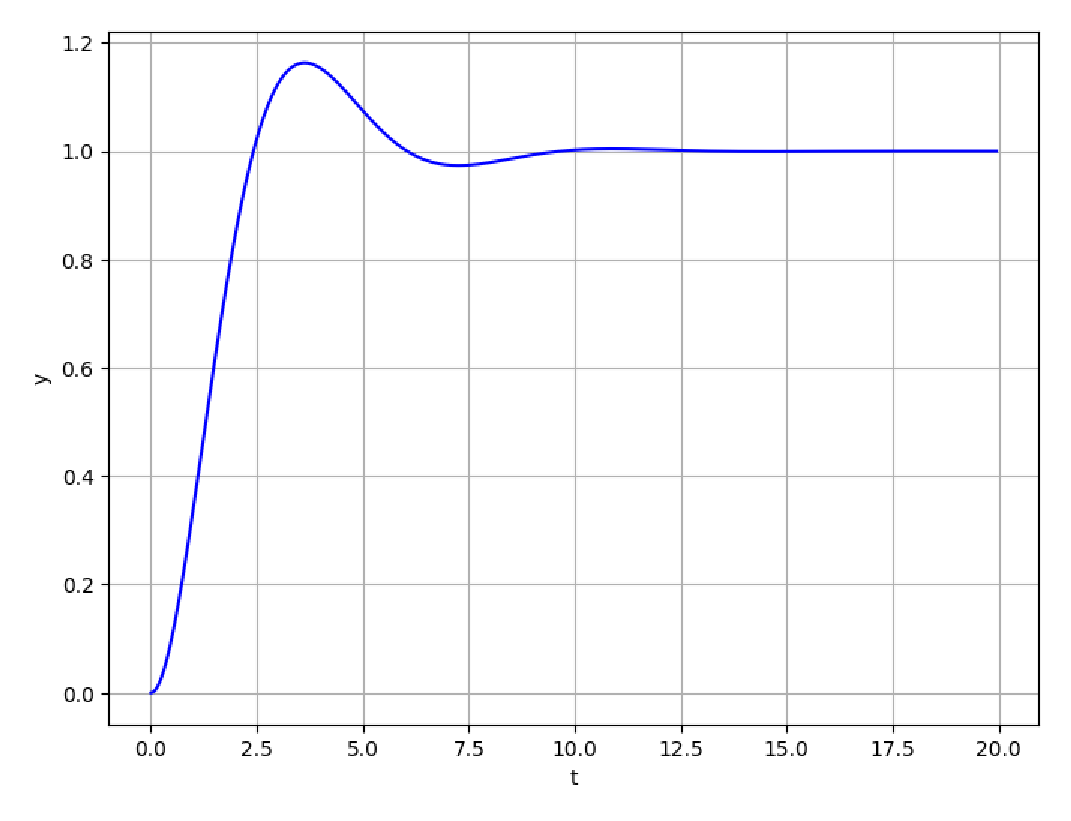
\includegraphics[scale=0.20]{figure2.eps}
    \vspace{25pt}\caption*{(a)}
    \label{}
  \end{minipage}
  \vspace{30pt}\begin{minipage}[h]{0.38\linewidth}
    \scalebox{0.5}[0.5]{
\begin{tikzpicture}[gnuplot]
%% generated with GNUPLOT 5.4p10 (Lua 5.4; terminal rev. Jun 2020, script rev. 118)
%% Sun Dec  3 22:33:05 2023
\path (0.000,0.000) rectangle (12.500,8.750);
\gpcolor{color=gp lt color border}
\gpsetlinetype{gp lt border}
\gpsetdashtype{gp dt solid}
\gpsetlinewidth{1.00}
\draw[gp path] (0.018,0.031)--(0.198,0.031);
\draw[gp path] (12.480,0.031)--(12.300,0.031);
\node[gp node right] at (-0.166,0.031) {$28$};
\draw[gp path] (0.018,0.996)--(0.198,0.996);
\draw[gp path] (12.480,0.996)--(12.300,0.996);
\node[gp node right] at (-0.166,0.996) {$29$};
\draw[gp path] (0.018,1.961)--(0.198,1.961);
\draw[gp path] (12.480,1.961)--(12.300,1.961);
\node[gp node right] at (-0.166,1.961) {$30$};
\draw[gp path] (0.018,2.927)--(0.198,2.927);
\draw[gp path] (12.480,2.927)--(12.300,2.927);
\node[gp node right] at (-0.166,2.927) {$31$};
\draw[gp path] (0.018,3.892)--(0.198,3.892);
\draw[gp path] (12.480,3.892)--(12.300,3.892);
\node[gp node right] at (-0.166,3.892) {$32$};
\draw[gp path] (0.018,4.857)--(0.198,4.857);
\draw[gp path] (12.480,4.857)--(12.300,4.857);
\node[gp node right] at (-0.166,4.857) {$33$};
\draw[gp path] (0.018,5.822)--(0.198,5.822);
\draw[gp path] (12.480,5.822)--(12.300,5.822);
\node[gp node right] at (-0.166,5.822) {$34$};
\draw[gp path] (0.018,6.788)--(0.198,6.788);
\draw[gp path] (12.480,6.788)--(12.300,6.788);
\node[gp node right] at (-0.166,6.788) {$35$};
\draw[gp path] (0.018,7.753)--(0.198,7.753);
\draw[gp path] (12.480,7.753)--(12.300,7.753);
\node[gp node right] at (-0.166,7.753) {$36$};
\draw[gp path] (0.018,8.718)--(0.198,8.718);
\draw[gp path] (12.480,8.718)--(12.300,8.718);
\node[gp node right] at (-0.166,8.718) {$37$};
\draw[gp path] (1.057,0.031)--(1.057,0.211);
\draw[gp path] (1.057,8.718)--(1.057,8.538);
\node[gp node center] at (1.057,-0.277) {$0$};
\draw[gp path] (3.134,0.031)--(3.134,0.211);
\draw[gp path] (3.134,8.718)--(3.134,8.538);
\node[gp node center] at (3.134,-0.277) {$1$};
\draw[gp path] (5.211,0.031)--(5.211,0.211);
\draw[gp path] (5.211,8.718)--(5.211,8.538);
\node[gp node center] at (5.211,-0.277) {$2$};
\draw[gp path] (7.288,0.031)--(7.288,0.211);
\draw[gp path] (7.288,8.718)--(7.288,8.538);
\node[gp node center] at (7.288,-0.277) {$3$};
\draw[gp path] (9.365,0.031)--(9.365,0.211);
\draw[gp path] (9.365,8.718)--(9.365,8.538);
\node[gp node center] at (9.365,-0.277) {$4$};
\draw[gp path] (11.442,0.031)--(11.442,0.211);
\draw[gp path] (11.442,8.718)--(11.442,8.538);
\node[gp node center] at (11.442,-0.277) {$5$};
\draw[gp path] (0.018,8.718)--(0.018,0.031)--(12.480,0.031)--(12.480,8.718)--cycle;
\node[gp node center,rotate=-270,font={\fontsize{17.0pt}{20.4pt}\selectfont}] at (-1.102,4.374) {$C_k$};
\node[gp node center,font={\fontsize{17.0pt}{20.4pt}\selectfont}] at (6.249,-1.046) {$k$};
\gpcolor{rgb color={0.000,0.000,0.000}}
\draw[gp path] (1.057,0.922)--(3.134,5.506)--(5.211,7.958)--(7.288,8.505)--(9.365,7.668)%
  --(11.442,5.898);
\gpsetpointsize{1.20}
\gp3point{gp mark 7}{}{(1.057,0.922)}
\gp3point{gp mark 7}{}{(3.134,5.506)}
\gp3point{gp mark 7}{}{(5.211,7.958)}
\gp3point{gp mark 7}{}{(7.288,8.505)}
\gp3point{gp mark 7}{}{(9.365,7.668)}
\gp3point{gp mark 7}{}{(11.442,5.898)}
\gpcolor{color=gp lt color border}
\draw[gp path] (0.018,8.718)--(0.018,0.031)--(12.480,0.031)--(12.480,8.718)--cycle;
%% coordinates of the plot area
\gpdefrectangularnode{gp plot 1}{\pgfpoint{0.018cm}{0.031cm}}{\pgfpoint{12.480cm}{8.718cm}}%% gnuplot variables
\end{tikzpicture}
}

    \vspace{-30pt}\caption*{(b)}
    \label{}
  \end{minipage}
  \vspace{-30pt}\caption{SI型について、(a)撮影したNFPの写真\ (b)光強度分布}
  \label{SI}
\end{figure}
図\ref{GI}から、GI型のコア径は$200\ \mathrm{\upmu m}$、図\ref{SI}から、SI型のコア径は$50\ \mathrm{\upmu m}$であることがわかる。\\
\\
{\large \bfseries 2.4 光ファイバの伝送帯域特性}\\
\begin{table}[h]
  \newcolumntype{I}{!{\vrule width 1.5pt}}
  \newcolumntype{i}{!{\vrule width 0.8pt}}
  \arrayrulewidth=0.8pt
  \renewcommand{\arraystretch}{1.5}
  \newcommand{\bhline}[1]{\noalign{\hrule height #1}}
  \centering
  \caption{光ファイバの出射光強度}
  \label{lengthefficiency}
  \begin{tabular}{IcicccI}
    \bhline{1.5pt}
    ファイバ被覆の色&ファイバ長\ /\ m&FWHM\ /\ ps&実測した伝送帯域\ /\ MHz\\
    \bhline{0.5pt}
    白色&100&769&956\\
    橙色&100&265&1100\\
    水色&100&129&2640\\
    \bhline{1.5pt}
  \end{tabular}
\end{table}
表\ref{lengthefficiency}と補足データからファイバ長とFWHMの関係を図\ref{fiberlength-FWHM}に、ファイバ長と伝送帯域の関係を図\ref{fiberlength-Hz}に示す。
\begin{figure}[h]
  \centering
  \scalebox{0.7}[0.7]{
\begin{tikzpicture}[gnuplot]
%% generated with GNUPLOT 5.4p10 (Lua 5.4; terminal rev. Jun 2020, script rev. 118)
%% Mon Dec 11 23:00:14 2023
\path (0.000,0.000) rectangle (12.500,8.750);
\gpcolor{color=gp lt color border}
\gpsetlinetype{gp lt border}
\gpsetdashtype{gp dt solid}
\gpsetlinewidth{1.00}
\draw[gp path] (0.018,0.031)--(0.198,0.031);
\node[gp node right] at (-0.166,0.031) {$0$};
\draw[gp path] (0.018,1.117)--(0.198,1.117);
\node[gp node right] at (-0.166,1.117) {$200$};
\draw[gp path] (0.018,2.203)--(0.198,2.203);
\node[gp node right] at (-0.166,2.203) {$400$};
\draw[gp path] (0.018,3.289)--(0.198,3.289);
\node[gp node right] at (-0.166,3.289) {$600$};
\draw[gp path] (0.018,4.375)--(0.198,4.375);
\node[gp node right] at (-0.166,4.375) {$800$};
\draw[gp path] (0.018,5.460)--(0.198,5.460);
\node[gp node right] at (-0.166,5.460) {$1000$};
\draw[gp path] (0.018,6.546)--(0.198,6.546);
\node[gp node right] at (-0.166,6.546) {$1200$};
\draw[gp path] (0.018,7.632)--(0.198,7.632);
\node[gp node right] at (-0.166,7.632) {$1400$};
\draw[gp path] (0.018,8.718)--(0.198,8.718);
\node[gp node right] at (-0.166,8.718) {$1600$};
\draw[gp path] (0.018,0.031)--(0.018,0.211);
\node[gp node center] at (0.018,-0.277) {$0$};
\draw[gp path] (1.403,0.031)--(1.403,0.211);
\node[gp node center] at (1.403,-0.277) {$20$};
\draw[gp path] (2.787,0.031)--(2.787,0.211);
\node[gp node center] at (2.787,-0.277) {$40$};
\draw[gp path] (4.172,0.031)--(4.172,0.211);
\node[gp node center] at (4.172,-0.277) {$60$};
\draw[gp path] (5.557,0.031)--(5.557,0.211);
\node[gp node center] at (5.557,-0.277) {$80$};
\draw[gp path] (6.941,0.031)--(6.941,0.211);
\node[gp node center] at (6.941,-0.277) {$100$};
\draw[gp path] (8.326,0.031)--(8.326,0.211);
\node[gp node center] at (8.326,-0.277) {$120$};
\draw[gp path] (9.711,0.031)--(9.711,0.211);
\node[gp node center] at (9.711,-0.277) {$140$};
\draw[gp path] (11.095,0.031)--(11.095,0.211);
\node[gp node center] at (11.095,-0.277) {$160$};
\draw[gp path] (12.480,0.031)--(12.480,0.211);
\node[gp node center] at (12.480,-0.277) {$180$};
\draw[gp path] (0.018,8.718)--(0.018,0.031)--(12.480,0.031)--(12.480,8.718)--cycle;
\node[gp node center,rotate=-270,font={\fontsize{17.0pt}{20.4pt}\selectfont}] at (-1.470,4.374) {FWHM$\ /\ \mathrm{ps}$};
\node[gp node center,font={\fontsize{17.0pt}{20.4pt}\selectfont}] at (6.249,-1.046) {ファイバ長$\ /\ \mathrm{m}$};
\node[gp node right] at (1.306,8.384) {白色};
\gpcolor{rgb color={0.745,0.745,0.745}}
\gpsetlinewidth{3.00}
\draw[gp path] (1.490,8.384)--(2.406,8.384);
\draw[gp path] (3.480,1.855)--(6.941,4.206)--(10.403,8.229);
\gpsetpointsize{3.20}
\gp3point{gp mark 7}{}{(3.480,1.855)}
\gp3point{gp mark 7}{}{(6.941,4.206)}
\gp3point{gp mark 7}{}{(10.403,8.229)}
\gp3point{gp mark 7}{}{(1.948,8.384)}
\gpcolor{color=gp lt color border}
\node[gp node right] at (1.306,8.076) {水色};
\gpcolor{rgb color={0.000,1.000,1.000}}
\draw[gp path] (1.490,8.076)--(2.406,8.076);
\draw[gp path] (3.480,0.549)--(6.941,0.731)--(10.403,0.693);
\gp3point{gp mark 7}{}{(3.480,0.549)}
\gp3point{gp mark 7}{}{(6.941,0.731)}
\gp3point{gp mark 7}{}{(10.403,0.693)}
\gp3point{gp mark 7}{}{(1.948,8.076)}
\gpcolor{color=gp lt color border}
\gpsetlinewidth{1.00}
\draw[gp path] (0.018,8.718)--(0.018,0.031)--(12.480,0.031)--(12.480,8.718)--cycle;
%% coordinates of the plot area
\gpdefrectangularnode{gp plot 1}{\pgfpoint{0.018cm}{0.031cm}}{\pgfpoint{12.480cm}{8.718cm}}
\end{tikzpicture}
}

  \vspace{-30pt}\caption{ファイバ長とFWHMの関係}
  \label{fiberlength-FWHM}
\end{figure}
\clearpage
\begin{figure}[h]
  \centering
  \scalebox{0.45}[0.45]{
\begin{tikzpicture}[gnuplot]
%% generated with GNUPLOT 5.4p10 (Lua 5.4; terminal rev. Jun 2020, script rev. 118)
%% Sun Nov 19 18:39:30 2023
\path (0.000,0.000) rectangle (12.500,8.750);
\gpcolor{color=gp lt color border}
\gpsetlinetype{gp lt border}
\gpsetdashtype{gp dt solid}
\gpsetlinewidth{1.00}
\draw[gp path] (0.018,0.031)--(0.198,0.031);
\draw[gp path] (12.480,0.031)--(12.300,0.031);
\node[gp node right] at (-0.166,0.031) {$0$};
\draw[gp path] (0.018,1.479)--(0.198,1.479);
\draw[gp path] (12.480,1.479)--(12.300,1.479);
\node[gp node right] at (-0.166,1.479) {$10$};
\draw[gp path] (0.018,2.927)--(0.198,2.927);
\draw[gp path] (12.480,2.927)--(12.300,2.927);
\node[gp node right] at (-0.166,2.927) {$20$};
\draw[gp path] (0.018,4.375)--(0.198,4.375);
\draw[gp path] (12.480,4.375)--(12.300,4.375);
\node[gp node right] at (-0.166,4.375) {$30$};
\draw[gp path] (0.018,5.822)--(0.198,5.822);
\draw[gp path] (12.480,5.822)--(12.300,5.822);
\node[gp node right] at (-0.166,5.822) {$40$};
\draw[gp path] (0.018,7.270)--(0.198,7.270);
\draw[gp path] (12.480,7.270)--(12.300,7.270);
\node[gp node right] at (-0.166,7.270) {$50$};
\draw[gp path] (0.018,8.718)--(0.198,8.718);
\draw[gp path] (12.480,8.718)--(12.300,8.718);
\node[gp node right] at (-0.166,8.718) {$60$};
\draw[gp path] (0.018,0.031)--(0.018,0.211);
\draw[gp path] (0.018,8.718)--(0.018,8.538);
\node[gp node center] at (0.018,-0.277) {$0$};
\draw[gp path] (2.284,0.031)--(2.284,0.211);
\draw[gp path] (2.284,8.718)--(2.284,8.538);
\node[gp node center] at (2.284,-0.277) {$2$};
\draw[gp path] (4.550,0.031)--(4.550,0.211);
\draw[gp path] (4.550,8.718)--(4.550,8.538);
\node[gp node center] at (4.550,-0.277) {$4$};
\draw[gp path] (6.815,0.031)--(6.815,0.211);
\draw[gp path] (6.815,8.718)--(6.815,8.538);
\node[gp node center] at (6.815,-0.277) {$6$};
\draw[gp path] (9.081,0.031)--(9.081,0.211);
\draw[gp path] (9.081,8.718)--(9.081,8.538);
\node[gp node center] at (9.081,-0.277) {$8$};
\draw[gp path] (11.347,0.031)--(11.347,0.211);
\draw[gp path] (11.347,8.718)--(11.347,8.538);
\node[gp node center] at (11.347,-0.277) {$10$};
\draw[gp path] (0.018,8.718)--(0.018,0.031)--(12.480,0.031)--(12.480,8.718)--cycle;
\node[gp node center,rotate=-270] at (-0.826,4.374) {ボールの位置$z\ /\ \mathrm{cm}$};
\node[gp node center] at (6.249,-0.738) {時間$t\ /\ \mathrm{s}$};
\gpcolor{rgb color={0.000,0.000,0.000}}
\draw[gp path] (0.018,0.312)--(0.041,1.203)--(0.063,2.405)--(0.086,3.428)--(0.109,4.115)%
  --(0.131,4.485)--(0.154,4.624)--(0.177,4.608)--(0.199,4.516)--(0.222,4.432)--(0.245,4.387)%
  --(0.267,4.373)--(0.290,4.360)--(0.313,4.328)--(0.335,4.304)--(0.358,4.297)--(0.381,4.287)%
  --(0.403,4.271)--(0.426,4.246)--(0.449,4.215)--(0.471,4.185)--(0.494,4.152)--(0.516,4.114)%
  --(0.539,4.078)--(0.562,4.051)--(0.584,4.035)--(0.607,4.027)--(0.630,4.030)--(0.652,4.045)%
  --(0.675,4.066)--(0.698,4.084)--(0.720,4.096)--(0.743,4.089)--(0.766,4.056)--(0.788,4.049)%
  --(0.811,4.115)--(0.834,4.224)--(0.856,4.334)--(0.879,4.417)--(0.902,4.463)--(0.924,4.472)%
  --(0.947,4.465)--(0.970,4.480)--(0.992,4.526)--(1.015,4.578)--(1.038,4.616)--(1.060,4.637)%
  --(1.083,4.645)--(1.106,4.646)--(1.128,4.548)--(1.151,4.333)--(1.174,4.203)--(1.196,4.234)%
  --(1.219,4.322)--(1.242,4.393)--(1.264,4.420)--(1.287,4.409)--(1.310,4.378)--(1.332,4.332)%
  --(1.355,4.277)--(1.377,4.209)--(1.400,4.123)--(1.423,4.045)--(1.445,3.992)--(1.468,3.955)%
  --(1.491,3.927)--(1.513,3.903)--(1.536,3.874)--(1.559,3.845)--(1.581,3.836)--(1.604,3.818)%
  --(1.627,3.774)--(1.649,3.743)--(1.672,3.736)--(1.695,3.731)--(1.717,3.714)--(1.740,3.701)%
  --(1.763,3.700)--(1.785,3.703)--(1.808,3.627)--(1.831,3.461)--(1.853,3.388)--(1.876,3.460)%
  --(1.899,3.565)--(1.921,3.640)--(1.944,3.689)--(1.967,3.724)--(1.989,3.757)--(2.012,3.799)%
  --(2.035,3.839)--(2.057,3.876)--(2.080,3.924)--(2.103,3.975)--(2.125,4.018)--(2.148,4.056)%
  --(2.171,4.087)--(2.193,4.086)--(2.216,4.046)--(2.239,4.019)--(2.261,4.032)--(2.284,4.070)%
  --(2.306,4.110)--(2.329,4.130)--(2.352,4.130)--(2.374,4.119)--(2.397,4.098)--(2.420,4.072)%
  --(2.442,4.051)--(2.465,4.028)--(2.488,3.992)--(2.510,3.949)--(2.533,3.905)--(2.556,3.859)%
  --(2.578,3.807)--(2.601,3.756)--(2.624,3.703)--(2.646,3.643)--(2.669,3.588)--(2.692,3.551)%
  --(2.714,3.532)--(2.737,3.510)--(2.760,3.480)--(2.782,3.449)--(2.805,3.422)--(2.828,3.402)%
  --(2.850,3.388)--(2.873,3.383)--(2.896,3.376)--(2.918,3.362)--(2.941,3.357)--(2.964,3.364)%
  --(2.986,3.242)--(3.009,2.973)--(3.032,2.843)--(3.054,2.938)--(3.077,3.122)--(3.100,3.315)%
  --(3.122,3.479)--(3.145,3.592)--(3.167,3.613)--(3.190,3.569)--(3.213,3.568)--(3.235,3.643)%
  --(3.258,3.747)--(3.281,3.850)--(3.303,3.933)--(3.326,3.996)--(3.349,4.042)--(3.371,4.073)%
  --(3.394,4.083)--(3.417,4.070)--(3.439,4.060)--(3.462,4.056)--(3.485,4.046)--(3.507,4.047)%
  --(3.530,4.064)--(3.553,4.084)--(3.575,4.100)--(3.598,4.103)--(3.621,4.087)--(3.643,4.034)%
  --(3.666,3.954)--(3.689,3.846)--(3.711,3.703)--(3.734,3.608)--(3.757,3.596)--(3.779,3.618)%
  --(3.802,3.645)--(3.825,3.611)--(3.847,3.510)--(3.870,3.446)--(3.893,3.456)--(3.915,3.496)%
  --(3.938,3.540)--(3.961,3.573)--(3.983,3.584)--(4.006,3.576)--(4.028,3.581)--(4.051,3.603)%
  --(4.074,3.625)--(4.096,3.647)--(4.119,3.668)--(4.142,3.679)--(4.164,3.681)--(4.187,3.698)%
  --(4.210,3.733)--(4.232,3.776)--(4.255,3.818)--(4.278,3.853)--(4.300,3.908)--(4.323,3.993)%
  --(4.346,4.082)--(4.368,4.144)--(4.391,4.170)--(4.414,4.173)--(4.436,4.157)--(4.459,4.153)%
  --(4.482,4.186)--(4.504,4.242)--(4.527,4.303)--(4.550,4.361)--(4.572,4.416)--(4.595,4.458)%
  --(4.618,4.479)--(4.640,4.484)--(4.663,4.477)--(4.686,4.474)--(4.708,4.487)--(4.731,4.498)%
  --(4.754,4.499)--(4.776,4.484)--(4.799,4.442)--(4.822,4.385)--(4.844,4.336)--(4.867,4.308)%
  --(4.890,4.312)--(4.912,4.348)--(4.935,4.396)--(4.957,4.460)--(4.980,4.530)--(5.003,4.559)%
  --(5.025,4.585)--(5.048,4.645)--(5.071,4.716)--(5.093,4.766)--(5.116,4.789)--(5.139,4.831)%
  --(5.161,4.887)--(5.184,4.899)--(5.207,4.882)--(5.229,4.915)--(5.252,5.009)--(5.275,5.111)%
  --(5.297,5.191)--(5.320,5.234)--(5.343,5.250)--(5.365,5.253)--(5.388,5.245)--(5.411,5.252)%
  --(5.433,5.268)--(5.456,5.268)--(5.479,5.276)--(5.501,5.304)--(5.524,5.334)--(5.547,5.353)%
  --(5.569,5.356)--(5.592,5.353)--(5.615,5.360)--(5.637,5.380)--(5.660,5.393)--(5.683,5.377)%
  --(5.705,5.325)--(5.728,5.253)--(5.751,5.155)--(5.773,5.044)--(5.796,4.990)--(5.818,5.007)%
  --(5.841,5.049)--(5.864,5.102)--(5.886,5.169)--(5.909,5.249)--(5.932,5.338)--(5.954,5.420)%
  --(5.977,5.459)--(6.000,5.437)--(6.022,5.389)--(6.045,5.356)--(6.068,5.353)--(6.090,5.406)%
  --(6.113,5.503)--(6.136,5.555)--(6.158,5.535)--(6.181,5.505)--(6.204,5.500)--(6.226,5.513)%
  --(6.249,5.521)--(6.272,5.526)--(6.294,5.545)--(6.317,5.560)--(6.340,5.555)--(6.362,5.538)%
  --(6.385,5.521)--(6.408,5.506)--(6.430,5.506)--(6.453,5.519)--(6.476,5.526)--(6.498,5.509)%
  --(6.521,5.466)--(6.544,5.417)--(6.566,5.382)--(6.589,5.362)--(6.612,5.354)--(6.634,5.340)%
  --(6.657,5.315)--(6.680,5.290)--(6.702,5.257)--(6.725,5.193)--(6.747,5.099)--(6.770,5.012)%
  --(6.793,4.927)--(6.815,4.829)--(6.838,4.768)--(6.861,4.762)--(6.883,4.782)--(6.906,4.807)%
  --(6.929,4.835)--(6.951,4.868)--(6.974,4.902)--(6.997,4.927)--(7.019,4.940)--(7.042,4.930)%
  --(7.065,4.886)--(7.087,4.839)--(7.110,4.843)--(7.133,4.933)--(7.155,5.064)--(7.178,5.178)%
  --(7.201,5.302)--(7.223,5.434)--(7.246,5.538)--(7.269,5.604)--(7.291,5.640)--(7.314,5.672)%
  --(7.337,5.707)--(7.359,5.731)--(7.382,5.745)--(7.405,5.801)--(7.427,5.968)--(7.450,6.281)%
  --(7.473,6.670)--(7.495,6.992)--(7.518,7.235)--(7.541,7.412)--(7.563,7.479)--(7.586,7.483)%
  --(7.608,7.539)--(7.631,7.657)--(7.654,7.753)--(7.676,7.796)--(7.699,7.817)--(7.722,7.841)%
  --(7.744,7.864)--(7.767,7.873)--(7.790,7.870)--(7.812,7.863)--(7.835,7.821)--(7.858,7.727)%
  --(7.880,7.348)--(7.903,6.663)--(7.926,6.303)--(7.948,6.460)--(7.971,6.799)--(7.994,7.132)%
  --(8.016,7.394)--(8.039,7.550)--(8.062,7.583)--(8.084,7.502)--(8.107,7.342)--(8.130,7.210)%
  --(8.152,7.176)--(8.175,7.248)--(8.198,7.372)--(8.220,7.487)--(8.243,7.566)--(8.266,7.556)%
  --(8.288,7.477)--(8.311,7.333)--(8.334,7.045)--(8.356,6.761)--(8.379,6.736)--(8.402,6.903)%
  --(8.424,7.033)--(8.447,7.027)--(8.470,7.012)--(8.492,7.149)--(8.515,7.270)--(8.537,7.237)%
  --(8.560,7.256)--(8.583,7.390)--(8.605,7.483)--(8.628,7.438)--(8.651,7.338)--(8.673,7.336)%
  --(8.696,7.423)--(8.719,7.523)--(8.741,7.613)--(8.764,7.598)--(8.787,7.445)--(8.809,7.325)%
  --(8.832,7.288)--(8.855,7.263)--(8.877,7.309)--(8.900,7.453)--(8.923,7.606)--(8.945,7.671)%
  --(8.968,7.634)--(8.991,7.566)--(9.013,7.455)--(9.036,7.328)--(9.059,7.318)--(9.081,7.381)%
  --(9.104,7.407)--(9.127,7.405)--(9.149,7.456)--(9.172,7.583)--(9.195,7.705)--(9.217,7.769)%
  --(9.240,7.770)--(9.263,7.743)--(9.285,7.713)--(9.308,7.674)--(9.331,7.623)--(9.353,7.566)%
  --(9.376,7.545)--(9.398,7.546)--(9.421,7.540)--(9.444,7.545)--(9.466,7.579)--(9.489,7.629)%
  --(9.512,7.685)--(9.534,7.732)--(9.557,7.757)--(9.580,7.670)--(9.602,7.335)--(9.625,6.782)%
  --(9.648,6.178)--(9.670,5.678)--(9.693,5.313)--(9.716,5.040)--(9.738,4.878)--(9.761,4.784)%
  --(9.784,4.662)--(9.806,4.497)--(9.829,4.310)--(9.852,4.183)--(9.874,4.207)--(9.897,4.368)%
  --(9.920,4.594)--(9.942,4.805)--(9.965,4.984)--(9.988,5.130)--(10.010,5.153)--(10.033,5.032)%
  --(10.056,4.899)--(10.078,4.764)--(10.101,4.539)--(10.124,4.271)--(10.146,4.031)--(10.169,3.860)%
  --(10.192,3.781)--(10.214,3.759)--(10.237,3.765)--(10.259,3.785)--(10.282,3.804)--(10.305,3.824)%
  --(10.327,3.844)--(10.350,3.853)--(10.373,3.853)--(10.395,3.860)--(10.418,3.872)--(10.441,3.882)%
  --(10.463,3.894)--(10.486,3.917)--(10.509,3.952)--(10.531,3.988)--(10.554,4.020)--(10.577,4.055)%
  --(10.599,4.097)--(10.622,4.147)--(10.645,4.204)--(10.667,4.270)--(10.690,4.333)--(10.713,4.354)%
  --(10.735,4.329)--(10.758,4.319)--(10.781,4.370)--(10.803,4.448)--(10.826,4.489)--(10.849,4.489)%
  --(10.871,4.492)--(10.894,4.502)--(10.917,4.507)--(10.939,4.504)--(10.962,4.494)--(10.985,4.461)%
  --(11.007,4.398)--(11.030,4.315)--(11.053,4.202)--(11.075,4.069)--(11.098,3.941)--(11.121,3.825)%
  --(11.143,3.717)--(11.166,3.613)--(11.188,3.512)--(11.211,3.414)--(11.234,3.318)--(11.256,3.222)%
  --(11.279,3.131)--(11.302,3.034)--(11.324,2.916)--(11.347,2.786)--(11.370,2.665)--(11.392,2.562)%
  --(11.415,2.480)--(11.438,2.409)--(11.460,2.342)--(11.483,2.278)--(11.506,2.217)--(11.528,2.161)%
  --(11.551,2.101)--(11.574,2.036)--(11.596,1.970)--(11.619,1.909)--(11.642,1.863)--(11.664,1.835)%
  --(11.687,1.815)--(11.710,1.800)--(11.732,1.783)--(11.755,1.762)--(11.778,1.741)--(11.800,1.724)%
  --(11.823,1.718)--(11.846,1.725)--(11.868,1.739)--(11.891,1.756)--(11.914,1.775)--(11.936,1.791)%
  --(11.959,1.802)--(11.982,1.826)--(12.004,1.857)--(12.027,1.887)--(12.049,1.930)--(12.072,1.986)%
  --(12.095,2.044)--(12.117,2.091)--(12.140,2.128)--(12.163,2.168)--(12.185,2.206)--(12.208,2.234)%
  --(12.231,2.253)--(12.253,2.258)--(12.276,2.251)--(12.299,2.230)--(12.321,2.197)--(12.344,2.154);
\gpsetpointsize{1.20}
\gp3point{gp mark 7}{}{(0.018,0.312)}
\gp3point{gp mark 7}{}{(0.041,1.203)}
\gp3point{gp mark 7}{}{(0.063,2.405)}
\gp3point{gp mark 7}{}{(0.086,3.428)}
\gp3point{gp mark 7}{}{(0.109,4.115)}
\gp3point{gp mark 7}{}{(0.131,4.485)}
\gp3point{gp mark 7}{}{(0.154,4.624)}
\gp3point{gp mark 7}{}{(0.177,4.608)}
\gp3point{gp mark 7}{}{(0.199,4.516)}
\gp3point{gp mark 7}{}{(0.222,4.432)}
\gp3point{gp mark 7}{}{(0.245,4.387)}
\gp3point{gp mark 7}{}{(0.267,4.373)}
\gp3point{gp mark 7}{}{(0.290,4.360)}
\gp3point{gp mark 7}{}{(0.313,4.328)}
\gp3point{gp mark 7}{}{(0.335,4.304)}
\gp3point{gp mark 7}{}{(0.358,4.297)}
\gp3point{gp mark 7}{}{(0.381,4.287)}
\gp3point{gp mark 7}{}{(0.403,4.271)}
\gp3point{gp mark 7}{}{(0.426,4.246)}
\gp3point{gp mark 7}{}{(0.449,4.215)}
\gp3point{gp mark 7}{}{(0.471,4.185)}
\gp3point{gp mark 7}{}{(0.494,4.152)}
\gp3point{gp mark 7}{}{(0.516,4.114)}
\gp3point{gp mark 7}{}{(0.539,4.078)}
\gp3point{gp mark 7}{}{(0.562,4.051)}
\gp3point{gp mark 7}{}{(0.584,4.035)}
\gp3point{gp mark 7}{}{(0.607,4.027)}
\gp3point{gp mark 7}{}{(0.630,4.030)}
\gp3point{gp mark 7}{}{(0.652,4.045)}
\gp3point{gp mark 7}{}{(0.675,4.066)}
\gp3point{gp mark 7}{}{(0.698,4.084)}
\gp3point{gp mark 7}{}{(0.720,4.096)}
\gp3point{gp mark 7}{}{(0.743,4.089)}
\gp3point{gp mark 7}{}{(0.766,4.056)}
\gp3point{gp mark 7}{}{(0.788,4.049)}
\gp3point{gp mark 7}{}{(0.811,4.115)}
\gp3point{gp mark 7}{}{(0.834,4.224)}
\gp3point{gp mark 7}{}{(0.856,4.334)}
\gp3point{gp mark 7}{}{(0.879,4.417)}
\gp3point{gp mark 7}{}{(0.902,4.463)}
\gp3point{gp mark 7}{}{(0.924,4.472)}
\gp3point{gp mark 7}{}{(0.947,4.465)}
\gp3point{gp mark 7}{}{(0.970,4.480)}
\gp3point{gp mark 7}{}{(0.992,4.526)}
\gp3point{gp mark 7}{}{(1.015,4.578)}
\gp3point{gp mark 7}{}{(1.038,4.616)}
\gp3point{gp mark 7}{}{(1.060,4.637)}
\gp3point{gp mark 7}{}{(1.083,4.645)}
\gp3point{gp mark 7}{}{(1.106,4.646)}
\gp3point{gp mark 7}{}{(1.128,4.548)}
\gp3point{gp mark 7}{}{(1.151,4.333)}
\gp3point{gp mark 7}{}{(1.174,4.203)}
\gp3point{gp mark 7}{}{(1.196,4.234)}
\gp3point{gp mark 7}{}{(1.219,4.322)}
\gp3point{gp mark 7}{}{(1.242,4.393)}
\gp3point{gp mark 7}{}{(1.264,4.420)}
\gp3point{gp mark 7}{}{(1.287,4.409)}
\gp3point{gp mark 7}{}{(1.310,4.378)}
\gp3point{gp mark 7}{}{(1.332,4.332)}
\gp3point{gp mark 7}{}{(1.355,4.277)}
\gp3point{gp mark 7}{}{(1.377,4.209)}
\gp3point{gp mark 7}{}{(1.400,4.123)}
\gp3point{gp mark 7}{}{(1.423,4.045)}
\gp3point{gp mark 7}{}{(1.445,3.992)}
\gp3point{gp mark 7}{}{(1.468,3.955)}
\gp3point{gp mark 7}{}{(1.491,3.927)}
\gp3point{gp mark 7}{}{(1.513,3.903)}
\gp3point{gp mark 7}{}{(1.536,3.874)}
\gp3point{gp mark 7}{}{(1.559,3.845)}
\gp3point{gp mark 7}{}{(1.581,3.836)}
\gp3point{gp mark 7}{}{(1.604,3.818)}
\gp3point{gp mark 7}{}{(1.627,3.774)}
\gp3point{gp mark 7}{}{(1.649,3.743)}
\gp3point{gp mark 7}{}{(1.672,3.736)}
\gp3point{gp mark 7}{}{(1.695,3.731)}
\gp3point{gp mark 7}{}{(1.717,3.714)}
\gp3point{gp mark 7}{}{(1.740,3.701)}
\gp3point{gp mark 7}{}{(1.763,3.700)}
\gp3point{gp mark 7}{}{(1.785,3.703)}
\gp3point{gp mark 7}{}{(1.808,3.627)}
\gp3point{gp mark 7}{}{(1.831,3.461)}
\gp3point{gp mark 7}{}{(1.853,3.388)}
\gp3point{gp mark 7}{}{(1.876,3.460)}
\gp3point{gp mark 7}{}{(1.899,3.565)}
\gp3point{gp mark 7}{}{(1.921,3.640)}
\gp3point{gp mark 7}{}{(1.944,3.689)}
\gp3point{gp mark 7}{}{(1.967,3.724)}
\gp3point{gp mark 7}{}{(1.989,3.757)}
\gp3point{gp mark 7}{}{(2.012,3.799)}
\gp3point{gp mark 7}{}{(2.035,3.839)}
\gp3point{gp mark 7}{}{(2.057,3.876)}
\gp3point{gp mark 7}{}{(2.080,3.924)}
\gp3point{gp mark 7}{}{(2.103,3.975)}
\gp3point{gp mark 7}{}{(2.125,4.018)}
\gp3point{gp mark 7}{}{(2.148,4.056)}
\gp3point{gp mark 7}{}{(2.171,4.087)}
\gp3point{gp mark 7}{}{(2.193,4.086)}
\gp3point{gp mark 7}{}{(2.216,4.046)}
\gp3point{gp mark 7}{}{(2.239,4.019)}
\gp3point{gp mark 7}{}{(2.261,4.032)}
\gp3point{gp mark 7}{}{(2.284,4.070)}
\gp3point{gp mark 7}{}{(2.306,4.110)}
\gp3point{gp mark 7}{}{(2.329,4.130)}
\gp3point{gp mark 7}{}{(2.352,4.130)}
\gp3point{gp mark 7}{}{(2.374,4.119)}
\gp3point{gp mark 7}{}{(2.397,4.098)}
\gp3point{gp mark 7}{}{(2.420,4.072)}
\gp3point{gp mark 7}{}{(2.442,4.051)}
\gp3point{gp mark 7}{}{(2.465,4.028)}
\gp3point{gp mark 7}{}{(2.488,3.992)}
\gp3point{gp mark 7}{}{(2.510,3.949)}
\gp3point{gp mark 7}{}{(2.533,3.905)}
\gp3point{gp mark 7}{}{(2.556,3.859)}
\gp3point{gp mark 7}{}{(2.578,3.807)}
\gp3point{gp mark 7}{}{(2.601,3.756)}
\gp3point{gp mark 7}{}{(2.624,3.703)}
\gp3point{gp mark 7}{}{(2.646,3.643)}
\gp3point{gp mark 7}{}{(2.669,3.588)}
\gp3point{gp mark 7}{}{(2.692,3.551)}
\gp3point{gp mark 7}{}{(2.714,3.532)}
\gp3point{gp mark 7}{}{(2.737,3.510)}
\gp3point{gp mark 7}{}{(2.760,3.480)}
\gp3point{gp mark 7}{}{(2.782,3.449)}
\gp3point{gp mark 7}{}{(2.805,3.422)}
\gp3point{gp mark 7}{}{(2.828,3.402)}
\gp3point{gp mark 7}{}{(2.850,3.388)}
\gp3point{gp mark 7}{}{(2.873,3.383)}
\gp3point{gp mark 7}{}{(2.896,3.376)}
\gp3point{gp mark 7}{}{(2.918,3.362)}
\gp3point{gp mark 7}{}{(2.941,3.357)}
\gp3point{gp mark 7}{}{(2.964,3.364)}
\gp3point{gp mark 7}{}{(2.986,3.242)}
\gp3point{gp mark 7}{}{(3.009,2.973)}
\gp3point{gp mark 7}{}{(3.032,2.843)}
\gp3point{gp mark 7}{}{(3.054,2.938)}
\gp3point{gp mark 7}{}{(3.077,3.122)}
\gp3point{gp mark 7}{}{(3.100,3.315)}
\gp3point{gp mark 7}{}{(3.122,3.479)}
\gp3point{gp mark 7}{}{(3.145,3.592)}
\gp3point{gp mark 7}{}{(3.167,3.613)}
\gp3point{gp mark 7}{}{(3.190,3.569)}
\gp3point{gp mark 7}{}{(3.213,3.568)}
\gp3point{gp mark 7}{}{(3.235,3.643)}
\gp3point{gp mark 7}{}{(3.258,3.747)}
\gp3point{gp mark 7}{}{(3.281,3.850)}
\gp3point{gp mark 7}{}{(3.303,3.933)}
\gp3point{gp mark 7}{}{(3.326,3.996)}
\gp3point{gp mark 7}{}{(3.349,4.042)}
\gp3point{gp mark 7}{}{(3.371,4.073)}
\gp3point{gp mark 7}{}{(3.394,4.083)}
\gp3point{gp mark 7}{}{(3.417,4.070)}
\gp3point{gp mark 7}{}{(3.439,4.060)}
\gp3point{gp mark 7}{}{(3.462,4.056)}
\gp3point{gp mark 7}{}{(3.485,4.046)}
\gp3point{gp mark 7}{}{(3.507,4.047)}
\gp3point{gp mark 7}{}{(3.530,4.064)}
\gp3point{gp mark 7}{}{(3.553,4.084)}
\gp3point{gp mark 7}{}{(3.575,4.100)}
\gp3point{gp mark 7}{}{(3.598,4.103)}
\gp3point{gp mark 7}{}{(3.621,4.087)}
\gp3point{gp mark 7}{}{(3.643,4.034)}
\gp3point{gp mark 7}{}{(3.666,3.954)}
\gp3point{gp mark 7}{}{(3.689,3.846)}
\gp3point{gp mark 7}{}{(3.711,3.703)}
\gp3point{gp mark 7}{}{(3.734,3.608)}
\gp3point{gp mark 7}{}{(3.757,3.596)}
\gp3point{gp mark 7}{}{(3.779,3.618)}
\gp3point{gp mark 7}{}{(3.802,3.645)}
\gp3point{gp mark 7}{}{(3.825,3.611)}
\gp3point{gp mark 7}{}{(3.847,3.510)}
\gp3point{gp mark 7}{}{(3.870,3.446)}
\gp3point{gp mark 7}{}{(3.893,3.456)}
\gp3point{gp mark 7}{}{(3.915,3.496)}
\gp3point{gp mark 7}{}{(3.938,3.540)}
\gp3point{gp mark 7}{}{(3.961,3.573)}
\gp3point{gp mark 7}{}{(3.983,3.584)}
\gp3point{gp mark 7}{}{(4.006,3.576)}
\gp3point{gp mark 7}{}{(4.028,3.581)}
\gp3point{gp mark 7}{}{(4.051,3.603)}
\gp3point{gp mark 7}{}{(4.074,3.625)}
\gp3point{gp mark 7}{}{(4.096,3.647)}
\gp3point{gp mark 7}{}{(4.119,3.668)}
\gp3point{gp mark 7}{}{(4.142,3.679)}
\gp3point{gp mark 7}{}{(4.164,3.681)}
\gp3point{gp mark 7}{}{(4.187,3.698)}
\gp3point{gp mark 7}{}{(4.210,3.733)}
\gp3point{gp mark 7}{}{(4.232,3.776)}
\gp3point{gp mark 7}{}{(4.255,3.818)}
\gp3point{gp mark 7}{}{(4.278,3.853)}
\gp3point{gp mark 7}{}{(4.300,3.908)}
\gp3point{gp mark 7}{}{(4.323,3.993)}
\gp3point{gp mark 7}{}{(4.346,4.082)}
\gp3point{gp mark 7}{}{(4.368,4.144)}
\gp3point{gp mark 7}{}{(4.391,4.170)}
\gp3point{gp mark 7}{}{(4.414,4.173)}
\gp3point{gp mark 7}{}{(4.436,4.157)}
\gp3point{gp mark 7}{}{(4.459,4.153)}
\gp3point{gp mark 7}{}{(4.482,4.186)}
\gp3point{gp mark 7}{}{(4.504,4.242)}
\gp3point{gp mark 7}{}{(4.527,4.303)}
\gp3point{gp mark 7}{}{(4.550,4.361)}
\gp3point{gp mark 7}{}{(4.572,4.416)}
\gp3point{gp mark 7}{}{(4.595,4.458)}
\gp3point{gp mark 7}{}{(4.618,4.479)}
\gp3point{gp mark 7}{}{(4.640,4.484)}
\gp3point{gp mark 7}{}{(4.663,4.477)}
\gp3point{gp mark 7}{}{(4.686,4.474)}
\gp3point{gp mark 7}{}{(4.708,4.487)}
\gp3point{gp mark 7}{}{(4.731,4.498)}
\gp3point{gp mark 7}{}{(4.754,4.499)}
\gp3point{gp mark 7}{}{(4.776,4.484)}
\gp3point{gp mark 7}{}{(4.799,4.442)}
\gp3point{gp mark 7}{}{(4.822,4.385)}
\gp3point{gp mark 7}{}{(4.844,4.336)}
\gp3point{gp mark 7}{}{(4.867,4.308)}
\gp3point{gp mark 7}{}{(4.890,4.312)}
\gp3point{gp mark 7}{}{(4.912,4.348)}
\gp3point{gp mark 7}{}{(4.935,4.396)}
\gp3point{gp mark 7}{}{(4.957,4.460)}
\gp3point{gp mark 7}{}{(4.980,4.530)}
\gp3point{gp mark 7}{}{(5.003,4.559)}
\gp3point{gp mark 7}{}{(5.025,4.585)}
\gp3point{gp mark 7}{}{(5.048,4.645)}
\gp3point{gp mark 7}{}{(5.071,4.716)}
\gp3point{gp mark 7}{}{(5.093,4.766)}
\gp3point{gp mark 7}{}{(5.116,4.789)}
\gp3point{gp mark 7}{}{(5.139,4.831)}
\gp3point{gp mark 7}{}{(5.161,4.887)}
\gp3point{gp mark 7}{}{(5.184,4.899)}
\gp3point{gp mark 7}{}{(5.207,4.882)}
\gp3point{gp mark 7}{}{(5.229,4.915)}
\gp3point{gp mark 7}{}{(5.252,5.009)}
\gp3point{gp mark 7}{}{(5.275,5.111)}
\gp3point{gp mark 7}{}{(5.297,5.191)}
\gp3point{gp mark 7}{}{(5.320,5.234)}
\gp3point{gp mark 7}{}{(5.343,5.250)}
\gp3point{gp mark 7}{}{(5.365,5.253)}
\gp3point{gp mark 7}{}{(5.388,5.245)}
\gp3point{gp mark 7}{}{(5.411,5.252)}
\gp3point{gp mark 7}{}{(5.433,5.268)}
\gp3point{gp mark 7}{}{(5.456,5.268)}
\gp3point{gp mark 7}{}{(5.479,5.276)}
\gp3point{gp mark 7}{}{(5.501,5.304)}
\gp3point{gp mark 7}{}{(5.524,5.334)}
\gp3point{gp mark 7}{}{(5.547,5.353)}
\gp3point{gp mark 7}{}{(5.569,5.356)}
\gp3point{gp mark 7}{}{(5.592,5.353)}
\gp3point{gp mark 7}{}{(5.615,5.360)}
\gp3point{gp mark 7}{}{(5.637,5.380)}
\gp3point{gp mark 7}{}{(5.660,5.393)}
\gp3point{gp mark 7}{}{(5.683,5.377)}
\gp3point{gp mark 7}{}{(5.705,5.325)}
\gp3point{gp mark 7}{}{(5.728,5.253)}
\gp3point{gp mark 7}{}{(5.751,5.155)}
\gp3point{gp mark 7}{}{(5.773,5.044)}
\gp3point{gp mark 7}{}{(5.796,4.990)}
\gp3point{gp mark 7}{}{(5.818,5.007)}
\gp3point{gp mark 7}{}{(5.841,5.049)}
\gp3point{gp mark 7}{}{(5.864,5.102)}
\gp3point{gp mark 7}{}{(5.886,5.169)}
\gp3point{gp mark 7}{}{(5.909,5.249)}
\gp3point{gp mark 7}{}{(5.932,5.338)}
\gp3point{gp mark 7}{}{(5.954,5.420)}
\gp3point{gp mark 7}{}{(5.977,5.459)}
\gp3point{gp mark 7}{}{(6.000,5.437)}
\gp3point{gp mark 7}{}{(6.022,5.389)}
\gp3point{gp mark 7}{}{(6.045,5.356)}
\gp3point{gp mark 7}{}{(6.068,5.353)}
\gp3point{gp mark 7}{}{(6.090,5.406)}
\gp3point{gp mark 7}{}{(6.113,5.503)}
\gp3point{gp mark 7}{}{(6.136,5.555)}
\gp3point{gp mark 7}{}{(6.158,5.535)}
\gp3point{gp mark 7}{}{(6.181,5.505)}
\gp3point{gp mark 7}{}{(6.204,5.500)}
\gp3point{gp mark 7}{}{(6.226,5.513)}
\gp3point{gp mark 7}{}{(6.249,5.521)}
\gp3point{gp mark 7}{}{(6.272,5.526)}
\gp3point{gp mark 7}{}{(6.294,5.545)}
\gp3point{gp mark 7}{}{(6.317,5.560)}
\gp3point{gp mark 7}{}{(6.340,5.555)}
\gp3point{gp mark 7}{}{(6.362,5.538)}
\gp3point{gp mark 7}{}{(6.385,5.521)}
\gp3point{gp mark 7}{}{(6.408,5.506)}
\gp3point{gp mark 7}{}{(6.430,5.506)}
\gp3point{gp mark 7}{}{(6.453,5.519)}
\gp3point{gp mark 7}{}{(6.476,5.526)}
\gp3point{gp mark 7}{}{(6.498,5.509)}
\gp3point{gp mark 7}{}{(6.521,5.466)}
\gp3point{gp mark 7}{}{(6.544,5.417)}
\gp3point{gp mark 7}{}{(6.566,5.382)}
\gp3point{gp mark 7}{}{(6.589,5.362)}
\gp3point{gp mark 7}{}{(6.612,5.354)}
\gp3point{gp mark 7}{}{(6.634,5.340)}
\gp3point{gp mark 7}{}{(6.657,5.315)}
\gp3point{gp mark 7}{}{(6.680,5.290)}
\gp3point{gp mark 7}{}{(6.702,5.257)}
\gp3point{gp mark 7}{}{(6.725,5.193)}
\gp3point{gp mark 7}{}{(6.747,5.099)}
\gp3point{gp mark 7}{}{(6.770,5.012)}
\gp3point{gp mark 7}{}{(6.793,4.927)}
\gp3point{gp mark 7}{}{(6.815,4.829)}
\gp3point{gp mark 7}{}{(6.838,4.768)}
\gp3point{gp mark 7}{}{(6.861,4.762)}
\gp3point{gp mark 7}{}{(6.883,4.782)}
\gp3point{gp mark 7}{}{(6.906,4.807)}
\gp3point{gp mark 7}{}{(6.929,4.835)}
\gp3point{gp mark 7}{}{(6.951,4.868)}
\gp3point{gp mark 7}{}{(6.974,4.902)}
\gp3point{gp mark 7}{}{(6.997,4.927)}
\gp3point{gp mark 7}{}{(7.019,4.940)}
\gp3point{gp mark 7}{}{(7.042,4.930)}
\gp3point{gp mark 7}{}{(7.065,4.886)}
\gp3point{gp mark 7}{}{(7.087,4.839)}
\gp3point{gp mark 7}{}{(7.110,4.843)}
\gp3point{gp mark 7}{}{(7.133,4.933)}
\gp3point{gp mark 7}{}{(7.155,5.064)}
\gp3point{gp mark 7}{}{(7.178,5.178)}
\gp3point{gp mark 7}{}{(7.201,5.302)}
\gp3point{gp mark 7}{}{(7.223,5.434)}
\gp3point{gp mark 7}{}{(7.246,5.538)}
\gp3point{gp mark 7}{}{(7.269,5.604)}
\gp3point{gp mark 7}{}{(7.291,5.640)}
\gp3point{gp mark 7}{}{(7.314,5.672)}
\gp3point{gp mark 7}{}{(7.337,5.707)}
\gp3point{gp mark 7}{}{(7.359,5.731)}
\gp3point{gp mark 7}{}{(7.382,5.745)}
\gp3point{gp mark 7}{}{(7.405,5.801)}
\gp3point{gp mark 7}{}{(7.427,5.968)}
\gp3point{gp mark 7}{}{(7.450,6.281)}
\gp3point{gp mark 7}{}{(7.473,6.670)}
\gp3point{gp mark 7}{}{(7.495,6.992)}
\gp3point{gp mark 7}{}{(7.518,7.235)}
\gp3point{gp mark 7}{}{(7.541,7.412)}
\gp3point{gp mark 7}{}{(7.563,7.479)}
\gp3point{gp mark 7}{}{(7.586,7.483)}
\gp3point{gp mark 7}{}{(7.608,7.539)}
\gp3point{gp mark 7}{}{(7.631,7.657)}
\gp3point{gp mark 7}{}{(7.654,7.753)}
\gp3point{gp mark 7}{}{(7.676,7.796)}
\gp3point{gp mark 7}{}{(7.699,7.817)}
\gp3point{gp mark 7}{}{(7.722,7.841)}
\gp3point{gp mark 7}{}{(7.744,7.864)}
\gp3point{gp mark 7}{}{(7.767,7.873)}
\gp3point{gp mark 7}{}{(7.790,7.870)}
\gp3point{gp mark 7}{}{(7.812,7.863)}
\gp3point{gp mark 7}{}{(7.835,7.821)}
\gp3point{gp mark 7}{}{(7.858,7.727)}
\gp3point{gp mark 7}{}{(7.880,7.348)}
\gp3point{gp mark 7}{}{(7.903,6.663)}
\gp3point{gp mark 7}{}{(7.926,6.303)}
\gp3point{gp mark 7}{}{(7.948,6.460)}
\gp3point{gp mark 7}{}{(7.971,6.799)}
\gp3point{gp mark 7}{}{(7.994,7.132)}
\gp3point{gp mark 7}{}{(8.016,7.394)}
\gp3point{gp mark 7}{}{(8.039,7.550)}
\gp3point{gp mark 7}{}{(8.062,7.583)}
\gp3point{gp mark 7}{}{(8.084,7.502)}
\gp3point{gp mark 7}{}{(8.107,7.342)}
\gp3point{gp mark 7}{}{(8.130,7.210)}
\gp3point{gp mark 7}{}{(8.152,7.176)}
\gp3point{gp mark 7}{}{(8.175,7.248)}
\gp3point{gp mark 7}{}{(8.198,7.372)}
\gp3point{gp mark 7}{}{(8.220,7.487)}
\gp3point{gp mark 7}{}{(8.243,7.566)}
\gp3point{gp mark 7}{}{(8.266,7.556)}
\gp3point{gp mark 7}{}{(8.288,7.477)}
\gp3point{gp mark 7}{}{(8.311,7.333)}
\gp3point{gp mark 7}{}{(8.334,7.045)}
\gp3point{gp mark 7}{}{(8.356,6.761)}
\gp3point{gp mark 7}{}{(8.379,6.736)}
\gp3point{gp mark 7}{}{(8.402,6.903)}
\gp3point{gp mark 7}{}{(8.424,7.033)}
\gp3point{gp mark 7}{}{(8.447,7.027)}
\gp3point{gp mark 7}{}{(8.470,7.012)}
\gp3point{gp mark 7}{}{(8.492,7.149)}
\gp3point{gp mark 7}{}{(8.515,7.270)}
\gp3point{gp mark 7}{}{(8.537,7.237)}
\gp3point{gp mark 7}{}{(8.560,7.256)}
\gp3point{gp mark 7}{}{(8.583,7.390)}
\gp3point{gp mark 7}{}{(8.605,7.483)}
\gp3point{gp mark 7}{}{(8.628,7.438)}
\gp3point{gp mark 7}{}{(8.651,7.338)}
\gp3point{gp mark 7}{}{(8.673,7.336)}
\gp3point{gp mark 7}{}{(8.696,7.423)}
\gp3point{gp mark 7}{}{(8.719,7.523)}
\gp3point{gp mark 7}{}{(8.741,7.613)}
\gp3point{gp mark 7}{}{(8.764,7.598)}
\gp3point{gp mark 7}{}{(8.787,7.445)}
\gp3point{gp mark 7}{}{(8.809,7.325)}
\gp3point{gp mark 7}{}{(8.832,7.288)}
\gp3point{gp mark 7}{}{(8.855,7.263)}
\gp3point{gp mark 7}{}{(8.877,7.309)}
\gp3point{gp mark 7}{}{(8.900,7.453)}
\gp3point{gp mark 7}{}{(8.923,7.606)}
\gp3point{gp mark 7}{}{(8.945,7.671)}
\gp3point{gp mark 7}{}{(8.968,7.634)}
\gp3point{gp mark 7}{}{(8.991,7.566)}
\gp3point{gp mark 7}{}{(9.013,7.455)}
\gp3point{gp mark 7}{}{(9.036,7.328)}
\gp3point{gp mark 7}{}{(9.059,7.318)}
\gp3point{gp mark 7}{}{(9.081,7.381)}
\gp3point{gp mark 7}{}{(9.104,7.407)}
\gp3point{gp mark 7}{}{(9.127,7.405)}
\gp3point{gp mark 7}{}{(9.149,7.456)}
\gp3point{gp mark 7}{}{(9.172,7.583)}
\gp3point{gp mark 7}{}{(9.195,7.705)}
\gp3point{gp mark 7}{}{(9.217,7.769)}
\gp3point{gp mark 7}{}{(9.240,7.770)}
\gp3point{gp mark 7}{}{(9.263,7.743)}
\gp3point{gp mark 7}{}{(9.285,7.713)}
\gp3point{gp mark 7}{}{(9.308,7.674)}
\gp3point{gp mark 7}{}{(9.331,7.623)}
\gp3point{gp mark 7}{}{(9.353,7.566)}
\gp3point{gp mark 7}{}{(9.376,7.545)}
\gp3point{gp mark 7}{}{(9.398,7.546)}
\gp3point{gp mark 7}{}{(9.421,7.540)}
\gp3point{gp mark 7}{}{(9.444,7.545)}
\gp3point{gp mark 7}{}{(9.466,7.579)}
\gp3point{gp mark 7}{}{(9.489,7.629)}
\gp3point{gp mark 7}{}{(9.512,7.685)}
\gp3point{gp mark 7}{}{(9.534,7.732)}
\gp3point{gp mark 7}{}{(9.557,7.757)}
\gp3point{gp mark 7}{}{(9.580,7.670)}
\gp3point{gp mark 7}{}{(9.602,7.335)}
\gp3point{gp mark 7}{}{(9.625,6.782)}
\gp3point{gp mark 7}{}{(9.648,6.178)}
\gp3point{gp mark 7}{}{(9.670,5.678)}
\gp3point{gp mark 7}{}{(9.693,5.313)}
\gp3point{gp mark 7}{}{(9.716,5.040)}
\gp3point{gp mark 7}{}{(9.738,4.878)}
\gp3point{gp mark 7}{}{(9.761,4.784)}
\gp3point{gp mark 7}{}{(9.784,4.662)}
\gp3point{gp mark 7}{}{(9.806,4.497)}
\gp3point{gp mark 7}{}{(9.829,4.310)}
\gp3point{gp mark 7}{}{(9.852,4.183)}
\gp3point{gp mark 7}{}{(9.874,4.207)}
\gp3point{gp mark 7}{}{(9.897,4.368)}
\gp3point{gp mark 7}{}{(9.920,4.594)}
\gp3point{gp mark 7}{}{(9.942,4.805)}
\gp3point{gp mark 7}{}{(9.965,4.984)}
\gp3point{gp mark 7}{}{(9.988,5.130)}
\gp3point{gp mark 7}{}{(10.010,5.153)}
\gp3point{gp mark 7}{}{(10.033,5.032)}
\gp3point{gp mark 7}{}{(10.056,4.899)}
\gp3point{gp mark 7}{}{(10.078,4.764)}
\gp3point{gp mark 7}{}{(10.101,4.539)}
\gp3point{gp mark 7}{}{(10.124,4.271)}
\gp3point{gp mark 7}{}{(10.146,4.031)}
\gp3point{gp mark 7}{}{(10.169,3.860)}
\gp3point{gp mark 7}{}{(10.192,3.781)}
\gp3point{gp mark 7}{}{(10.214,3.759)}
\gp3point{gp mark 7}{}{(10.237,3.765)}
\gp3point{gp mark 7}{}{(10.259,3.785)}
\gp3point{gp mark 7}{}{(10.282,3.804)}
\gp3point{gp mark 7}{}{(10.305,3.824)}
\gp3point{gp mark 7}{}{(10.327,3.844)}
\gp3point{gp mark 7}{}{(10.350,3.853)}
\gp3point{gp mark 7}{}{(10.373,3.853)}
\gp3point{gp mark 7}{}{(10.395,3.860)}
\gp3point{gp mark 7}{}{(10.418,3.872)}
\gp3point{gp mark 7}{}{(10.441,3.882)}
\gp3point{gp mark 7}{}{(10.463,3.894)}
\gp3point{gp mark 7}{}{(10.486,3.917)}
\gp3point{gp mark 7}{}{(10.509,3.952)}
\gp3point{gp mark 7}{}{(10.531,3.988)}
\gp3point{gp mark 7}{}{(10.554,4.020)}
\gp3point{gp mark 7}{}{(10.577,4.055)}
\gp3point{gp mark 7}{}{(10.599,4.097)}
\gp3point{gp mark 7}{}{(10.622,4.147)}
\gp3point{gp mark 7}{}{(10.645,4.204)}
\gp3point{gp mark 7}{}{(10.667,4.270)}
\gp3point{gp mark 7}{}{(10.690,4.333)}
\gp3point{gp mark 7}{}{(10.713,4.354)}
\gp3point{gp mark 7}{}{(10.735,4.329)}
\gp3point{gp mark 7}{}{(10.758,4.319)}
\gp3point{gp mark 7}{}{(10.781,4.370)}
\gp3point{gp mark 7}{}{(10.803,4.448)}
\gp3point{gp mark 7}{}{(10.826,4.489)}
\gp3point{gp mark 7}{}{(10.849,4.489)}
\gp3point{gp mark 7}{}{(10.871,4.492)}
\gp3point{gp mark 7}{}{(10.894,4.502)}
\gp3point{gp mark 7}{}{(10.917,4.507)}
\gp3point{gp mark 7}{}{(10.939,4.504)}
\gp3point{gp mark 7}{}{(10.962,4.494)}
\gp3point{gp mark 7}{}{(10.985,4.461)}
\gp3point{gp mark 7}{}{(11.007,4.398)}
\gp3point{gp mark 7}{}{(11.030,4.315)}
\gp3point{gp mark 7}{}{(11.053,4.202)}
\gp3point{gp mark 7}{}{(11.075,4.069)}
\gp3point{gp mark 7}{}{(11.098,3.941)}
\gp3point{gp mark 7}{}{(11.121,3.825)}
\gp3point{gp mark 7}{}{(11.143,3.717)}
\gp3point{gp mark 7}{}{(11.166,3.613)}
\gp3point{gp mark 7}{}{(11.188,3.512)}
\gp3point{gp mark 7}{}{(11.211,3.414)}
\gp3point{gp mark 7}{}{(11.234,3.318)}
\gp3point{gp mark 7}{}{(11.256,3.222)}
\gp3point{gp mark 7}{}{(11.279,3.131)}
\gp3point{gp mark 7}{}{(11.302,3.034)}
\gp3point{gp mark 7}{}{(11.324,2.916)}
\gp3point{gp mark 7}{}{(11.347,2.786)}
\gp3point{gp mark 7}{}{(11.370,2.665)}
\gp3point{gp mark 7}{}{(11.392,2.562)}
\gp3point{gp mark 7}{}{(11.415,2.480)}
\gp3point{gp mark 7}{}{(11.438,2.409)}
\gp3point{gp mark 7}{}{(11.460,2.342)}
\gp3point{gp mark 7}{}{(11.483,2.278)}
\gp3point{gp mark 7}{}{(11.506,2.217)}
\gp3point{gp mark 7}{}{(11.528,2.161)}
\gp3point{gp mark 7}{}{(11.551,2.101)}
\gp3point{gp mark 7}{}{(11.574,2.036)}
\gp3point{gp mark 7}{}{(11.596,1.970)}
\gp3point{gp mark 7}{}{(11.619,1.909)}
\gp3point{gp mark 7}{}{(11.642,1.863)}
\gp3point{gp mark 7}{}{(11.664,1.835)}
\gp3point{gp mark 7}{}{(11.687,1.815)}
\gp3point{gp mark 7}{}{(11.710,1.800)}
\gp3point{gp mark 7}{}{(11.732,1.783)}
\gp3point{gp mark 7}{}{(11.755,1.762)}
\gp3point{gp mark 7}{}{(11.778,1.741)}
\gp3point{gp mark 7}{}{(11.800,1.724)}
\gp3point{gp mark 7}{}{(11.823,1.718)}
\gp3point{gp mark 7}{}{(11.846,1.725)}
\gp3point{gp mark 7}{}{(11.868,1.739)}
\gp3point{gp mark 7}{}{(11.891,1.756)}
\gp3point{gp mark 7}{}{(11.914,1.775)}
\gp3point{gp mark 7}{}{(11.936,1.791)}
\gp3point{gp mark 7}{}{(11.959,1.802)}
\gp3point{gp mark 7}{}{(11.982,1.826)}
\gp3point{gp mark 7}{}{(12.004,1.857)}
\gp3point{gp mark 7}{}{(12.027,1.887)}
\gp3point{gp mark 7}{}{(12.049,1.930)}
\gp3point{gp mark 7}{}{(12.072,1.986)}
\gp3point{gp mark 7}{}{(12.095,2.044)}
\gp3point{gp mark 7}{}{(12.117,2.091)}
\gp3point{gp mark 7}{}{(12.140,2.128)}
\gp3point{gp mark 7}{}{(12.163,2.168)}
\gp3point{gp mark 7}{}{(12.185,2.206)}
\gp3point{gp mark 7}{}{(12.208,2.234)}
\gp3point{gp mark 7}{}{(12.231,2.253)}
\gp3point{gp mark 7}{}{(12.253,2.258)}
\gp3point{gp mark 7}{}{(12.276,2.251)}
\gp3point{gp mark 7}{}{(12.299,2.230)}
\gp3point{gp mark 7}{}{(12.321,2.197)}
\gp3point{gp mark 7}{}{(12.344,2.154)}
\gpcolor{color=gp lt color border}
\draw[gp path] (0.018,8.718)--(0.018,0.031)--(12.480,0.031)--(12.480,8.718)--cycle;
%% coordinates of the plot area
\gpdefrectangularnode{gp plot 1}{\pgfpoint{0.018cm}{0.031cm}}{\pgfpoint{12.480cm}{8.718cm}}
\end{tikzpicture}
%% gnuplot variables
}

  \vspace{-30pt}\caption{ファイバ長と伝送帯域の関係}
  \label{fiberlength-Hz}
\end{figure}
 図\ref{fiberlength-FWHM}から、水色のFWHMはファイバ長に対してほぼ一定、白色のFWHMはファイバ長と正の相関があることがわかる。また、図\ref{fiberlength-Hz}から、水色の伝送帯域は白色の伝送帯域よりも大きくなった。そして両方の伝送帯域がファイバの長さに反比例した。
\begin{figure}[h]
  \centering
  \vspace{20pt}\begin{minipage}[h]{0.8\linewidth}
    \begin{minipage}[h]{0.53\linewidth}
      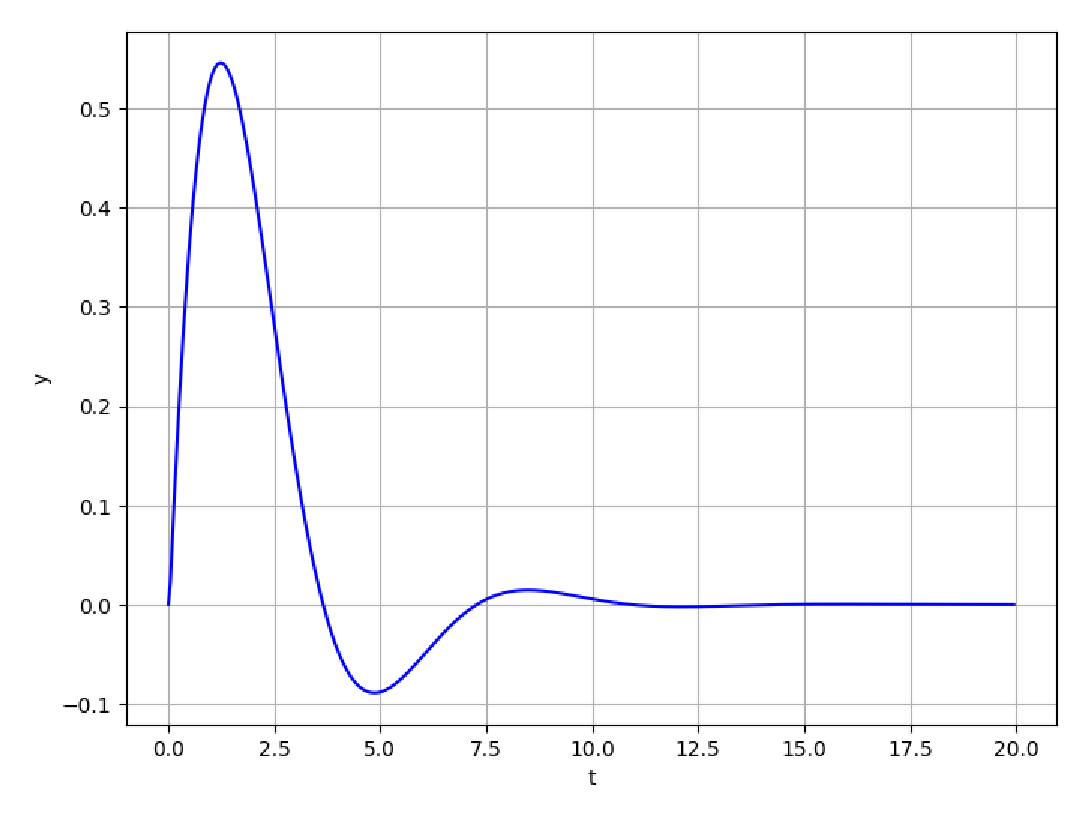
\includegraphics[scale=0.05]{figure3.eps}
    \end{minipage}
    \begin{minipage}[h]{0.5\linewidth}
      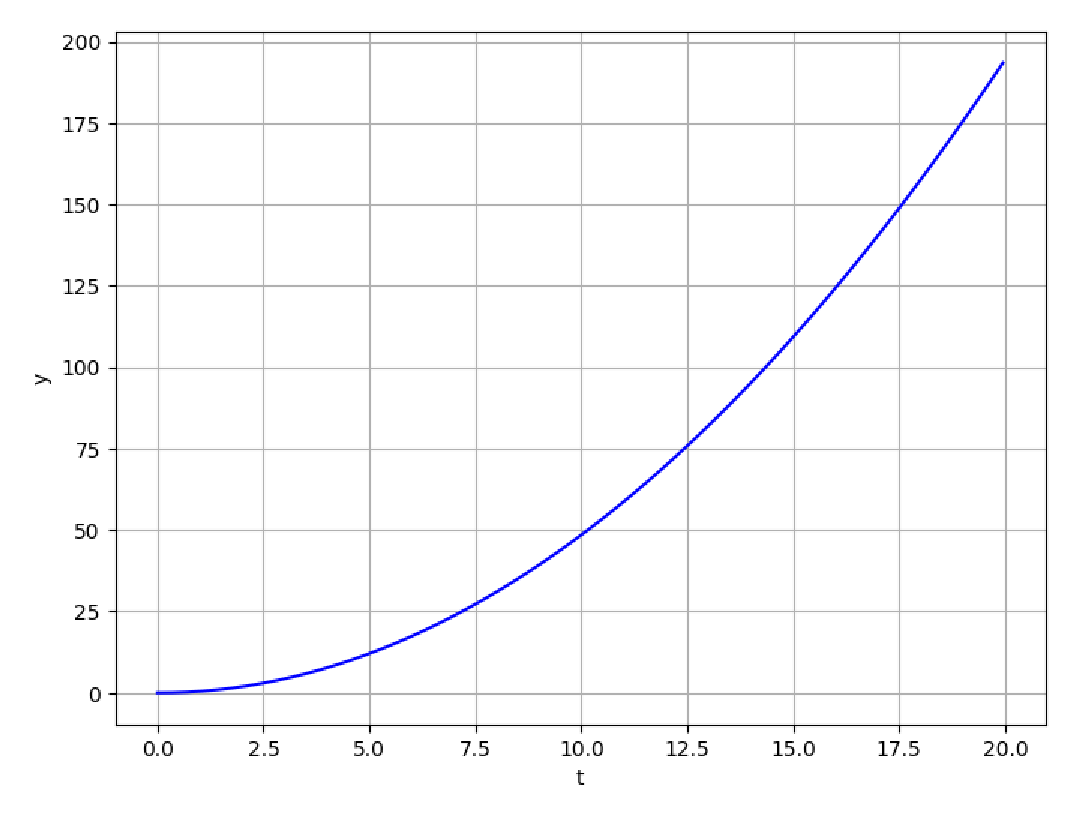
\includegraphics[scale=0.05]{figure4.eps}
    \end{minipage}
    \caption*{(a)}
  \end{minipage}
  \begin{minipage}[h]{0.8\linewidth}
    \begin{minipage}[h]{0.53\linewidth}
      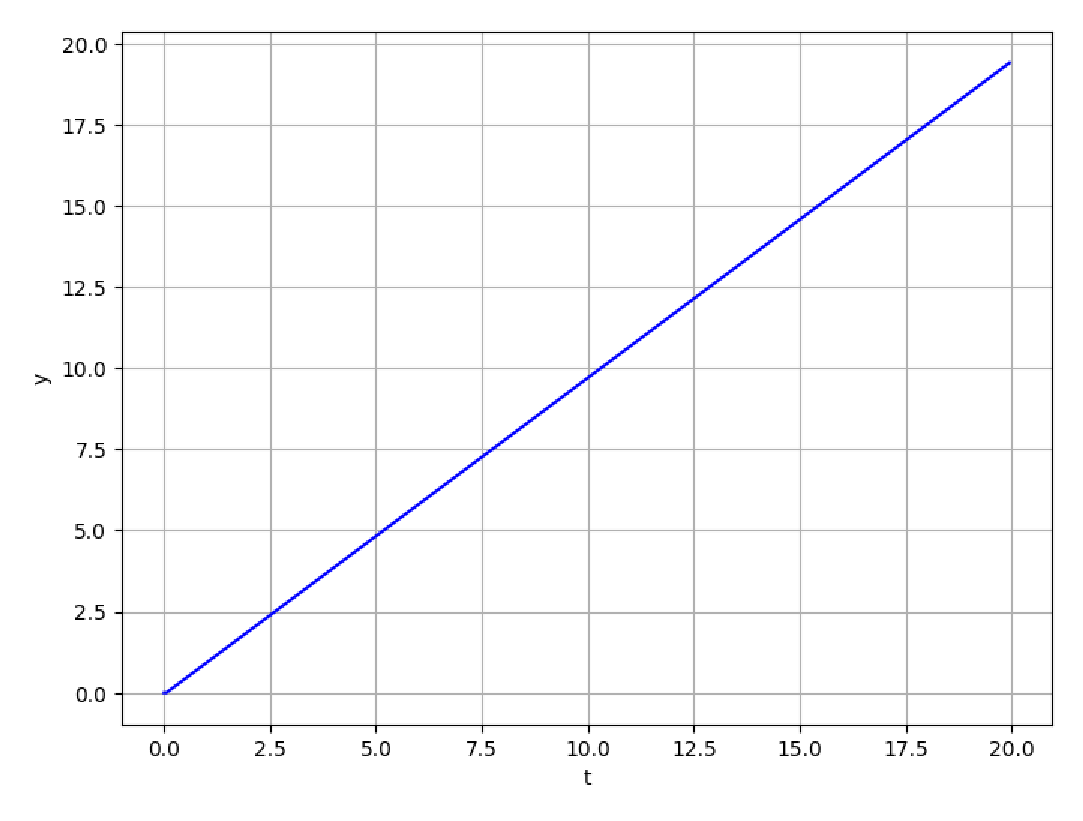
\includegraphics[scale=0.05]{figure5.eps}
    \end{minipage}
    \begin{minipage}[h]{0.5\linewidth}
      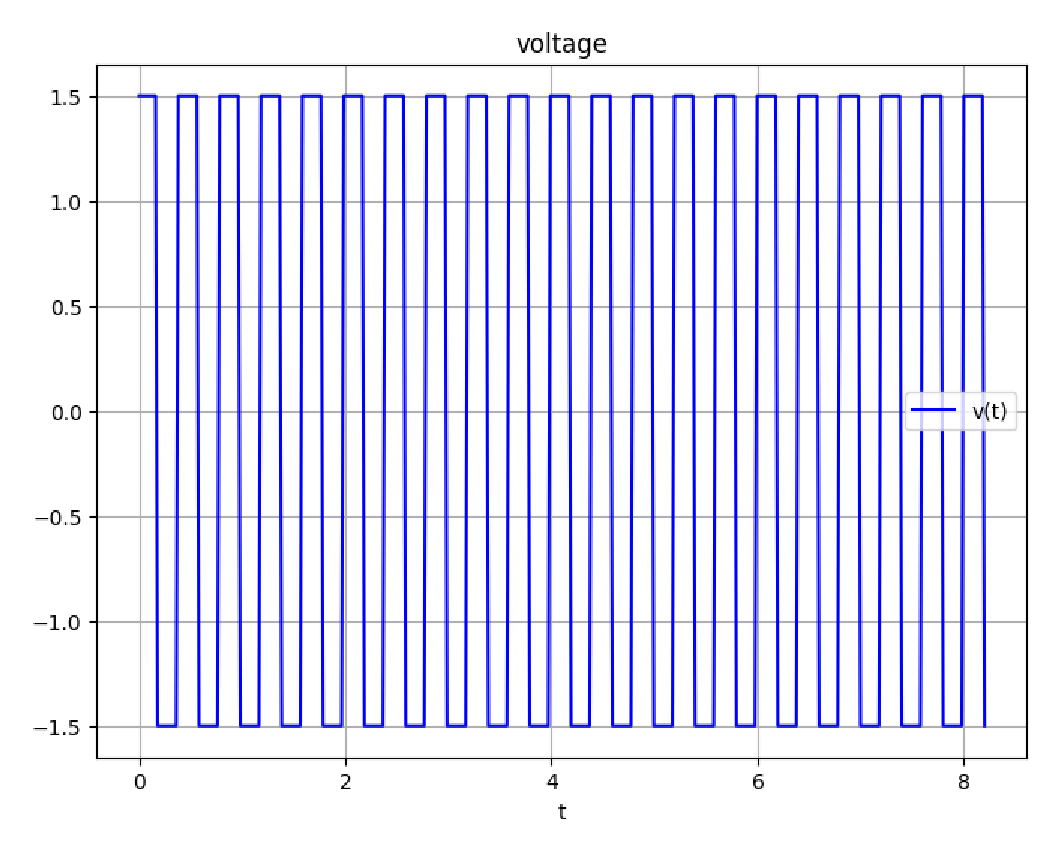
\includegraphics[scale=0.05]{figure6.eps}
    \end{minipage}
    \caption*{(b)}
  \end{minipage}
  \begin{minipage}[h]{0.8\linewidth}
    \begin{minipage}[h]{0.53\linewidth}
      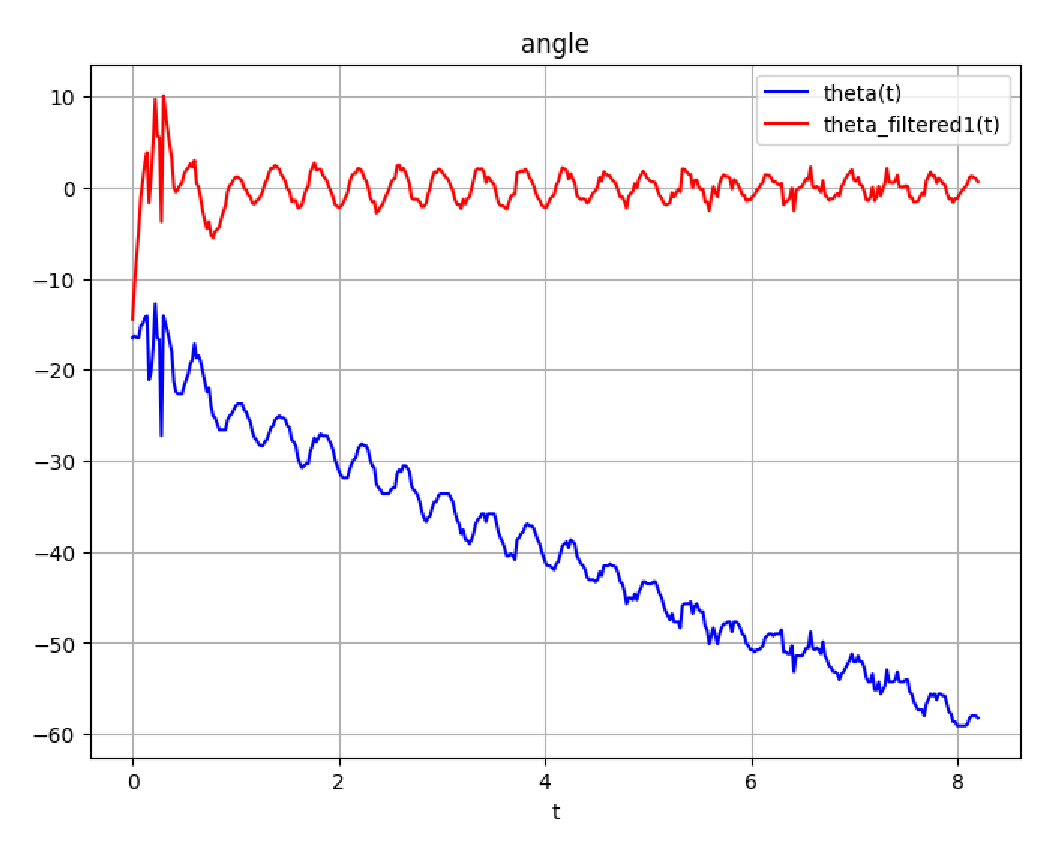
\includegraphics[scale=0.05]{figure7.eps}
    \end{minipage}
    \begin{minipage}[h]{0.5\linewidth}
      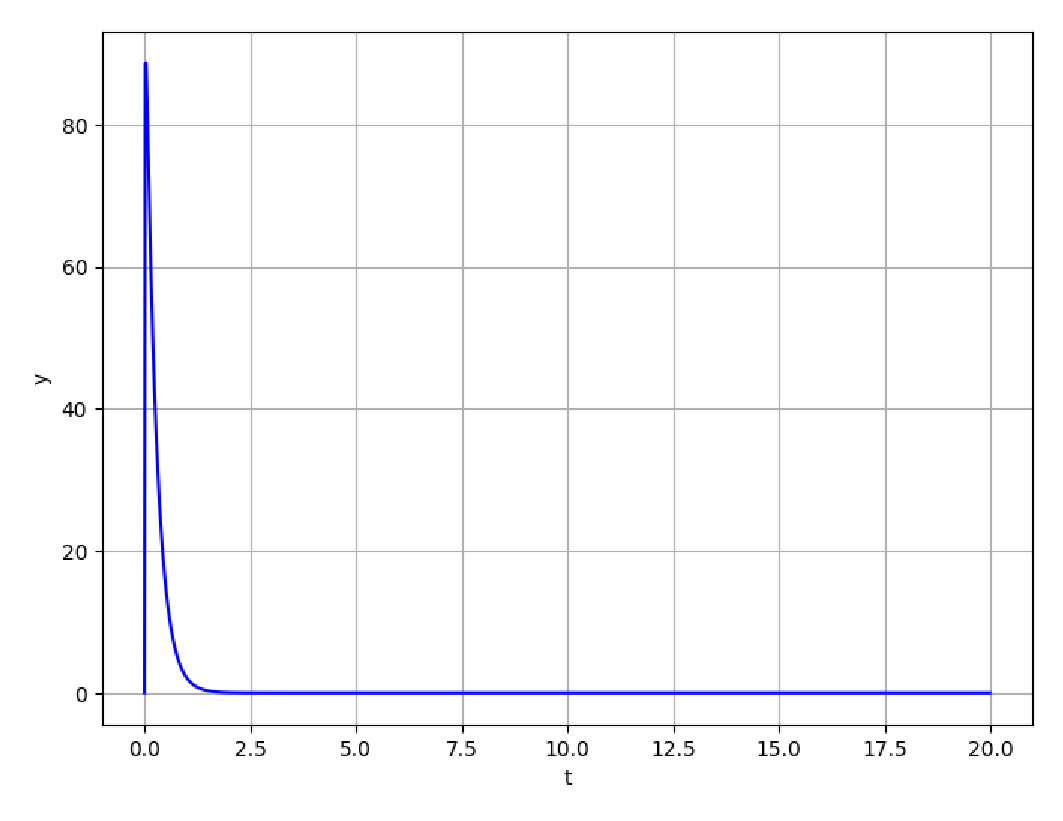
\includegraphics[scale=0.05]{figure8.eps}
    \end{minipage}
    \caption*{(c)}
  \end{minipage}
  \caption{オシロスコープ(a)白色の光ファイバー、(b)橙色の光ファイバー、(c)水色の光ファイバー}
  \label{scope}
\end{figure}
\clearpage
\hspace{-2pt}{\Large \bfseries 3.考察}\\
{\large \bfseries 3.1光ファイバの種類と構造}\\
 光ファイバの種類には、シングルモードファイバ、SI型のマルチモードファイバ、GI型のマルチモードファイバが存在する。シングルモードファイバはコア径が$8〜10\ \mathrm{\upmu m}$で小さく、単一方向つまり光ファイバーに平行な向きの光しか伝送できない。しかし、シングルモードの光しか伝送できないことから原理的にモード分散が存在せず、長距離の光伝送に向いている。マルチモードファイバはコア径が$50〜62.5\ \mathrm{\upmu m}$である。このうち、SI型はコア全体の屈折率が一定で入射した光はコアとクラッドの境目で全反射を繰り返しながら伝送される。また、コア径が大きいため複数の方向の光を伝送することができる。しかし、クラッドへの入射が小さい光は光路長がクラッドへの入射角が大きい光より長くなり、モード分散が大きくなる。これを改善するために作られた光ファイバがGI型のマルチモードファイバで、SI型と違ってコアの屈折率が中心から外側に向かって小さくなるようになっている。これにより、クラッドへの入射角の大きい光は屈折率の大きい領域を通過する時間が長くなり、逆にクラッドへの入射角の小さい光は屈折率の大きい領域と小さい領域を通り、最終的にどのモードの光も同じぐらいのタイミングで伝送先へ到着する。そのため、GI型はモード分散が小さい。このようなことから、シングルモードファイバは大陸間のような長距離の伝送、マルチモードファイバは家庭内のような短距離の伝送で用いられる。\\
\\
{\large \bfseries 3.2光結合特性}\\
 図\ref{core-efficiency}にコア面積と結合効率の関係を示す。ただし、点は表\ref{efficiency}での測定点、直線はそれらの回帰直線を表す。
\begin{figure}[h]
  \centering
  \scalebox{0.45}[0.45]{
\begin{tikzpicture}[gnuplot]
%% generated with GNUPLOT 5.4p10 (Lua 5.4; terminal rev. Jun 2020, script rev. 118)
%% Sun Nov 19 18:02:42 2023
\path (0.000,0.000) rectangle (12.500,8.750);
\gpcolor{color=gp lt color border}
\gpsetlinetype{gp lt border}
\gpsetdashtype{gp dt solid}
\gpsetlinewidth{1.00}
\draw[gp path] (0.018,0.031)--(0.198,0.031);
\draw[gp path] (12.480,0.031)--(12.300,0.031);
\node[gp node right] at (-0.166,0.031) {$-100$};
\draw[gp path] (0.018,1.768)--(0.198,1.768);
\draw[gp path] (12.480,1.768)--(12.300,1.768);
\node[gp node right] at (-0.166,1.768) {$-50$};
\draw[gp path] (0.018,3.506)--(0.198,3.506);
\draw[gp path] (12.480,3.506)--(12.300,3.506);
\node[gp node right] at (-0.166,3.506) {$0$};
\draw[gp path] (0.018,5.243)--(0.198,5.243);
\draw[gp path] (12.480,5.243)--(12.300,5.243);
\node[gp node right] at (-0.166,5.243) {$50$};
\draw[gp path] (0.018,6.981)--(0.198,6.981);
\draw[gp path] (12.480,6.981)--(12.300,6.981);
\node[gp node right] at (-0.166,6.981) {$100$};
\draw[gp path] (0.018,8.718)--(0.198,8.718);
\draw[gp path] (12.480,8.718)--(12.300,8.718);
\node[gp node right] at (-0.166,8.718) {$150$};
\draw[gp path] (0.018,0.031)--(0.018,0.211);
\draw[gp path] (0.018,8.718)--(0.018,8.538);
\node[gp node center] at (0.018,-0.277) {$0$};
\draw[gp path] (2.510,0.031)--(2.510,0.211);
\draw[gp path] (2.510,8.718)--(2.510,8.538);
\node[gp node center] at (2.510,-0.277) {$5$};
\draw[gp path] (5.003,0.031)--(5.003,0.211);
\draw[gp path] (5.003,8.718)--(5.003,8.538);
\node[gp node center] at (5.003,-0.277) {$10$};
\draw[gp path] (7.495,0.031)--(7.495,0.211);
\draw[gp path] (7.495,8.718)--(7.495,8.538);
\node[gp node center] at (7.495,-0.277) {$15$};
\draw[gp path] (9.988,0.031)--(9.988,0.211);
\draw[gp path] (9.988,8.718)--(9.988,8.538);
\node[gp node center] at (9.988,-0.277) {$20$};
\draw[gp path] (12.480,0.031)--(12.480,0.211);
\draw[gp path] (12.480,8.718)--(12.480,8.538);
\node[gp node center] at (12.480,-0.277) {$25$};
\draw[gp path] (0.018,8.718)--(0.018,0.031)--(12.480,0.031)--(12.480,8.718)--cycle;
\node[gp node center,rotate=-270] at (-1.194,4.374) {角度$\theta\ /\ ^\circ$};
\node[gp node center] at (6.249,-0.738) {時間$t\ /\ \mathrm{s}$};
\gpcolor{rgb color={0.000,0.000,0.000}}
\draw[gp path] (0.018,3.552)--(0.028,3.552)--(0.038,3.552)--(0.048,3.521)--(0.058,3.460)%
  --(0.068,3.399)--(0.078,3.277)--(0.088,3.162)--(0.098,3.040)--(0.108,2.864)--(0.118,2.658)%
  --(0.128,2.223)--(0.138,2.651)--(0.148,2.826)--(0.158,3.124)--(0.168,3.208)--(0.178,3.414)%
  --(0.187,3.567)--(0.197,3.735)--(0.207,3.880)--(0.217,4.094)--(0.227,4.223)--(0.237,4.323)%
  --(0.247,4.430)--(0.257,4.346)--(0.267,4.185)--(0.277,4.033)--(0.287,3.849)--(0.297,3.704)%
  --(0.307,3.628)--(0.317,3.536)--(0.327,3.475)--(0.337,3.422)--(0.347,3.399)--(0.357,3.361)%
  --(0.367,3.353)--(0.377,3.284)--(0.387,3.292)--(0.397,3.300)--(0.407,3.323)--(0.417,3.330)%
  --(0.427,3.353)--(0.437,3.353)--(0.447,3.407)--(0.457,3.422)--(0.467,3.414)--(0.477,3.422)%
  --(0.487,3.414)--(0.497,3.414)--(0.507,3.407)--(0.516,3.422)--(0.526,3.491)--(0.536,3.544)%
  --(0.546,3.605)--(0.556,3.636)--(0.566,3.659)--(0.576,3.651)--(0.586,3.651)--(0.596,3.651)%
  --(0.606,3.651)--(0.616,3.651)--(0.626,3.643)--(0.636,3.643)--(0.646,3.643)--(0.656,3.651)%
  --(0.666,3.651)--(0.676,3.651)--(0.686,3.651)--(0.696,3.636)--(0.706,3.597)--(0.716,3.475)%
  --(0.726,3.284)--(0.736,3.177)--(0.746,3.025)--(0.756,2.849)--(0.766,2.750)--(0.776,2.643)%
  --(0.786,2.582)--(0.796,2.452)--(0.806,2.391)--(0.816,2.330)--(0.826,2.330)--(0.836,2.345)%
  --(0.845,2.460)--(0.855,2.536)--(0.865,2.582)--(0.875,2.727)--(0.885,2.811)--(0.895,2.849)%
  --(0.905,2.994)--(0.915,3.116)--(0.925,3.208)--(0.935,3.338)--(0.945,3.613)--(0.955,3.872)%
  --(0.965,4.048)--(0.975,4.231)--(0.985,4.338)--(0.995,4.353)--(1.005,4.338)--(1.015,4.292)%
  --(1.025,4.208)--(1.035,4.101)--(1.045,3.987)--(1.055,3.895)--(1.065,3.781)--(1.075,3.689)%
  --(1.085,3.628)--(1.095,3.590)--(1.105,3.567)--(1.115,3.559)--(1.125,3.552)--(1.135,3.552)%
  --(1.145,3.552)--(1.155,3.552)--(1.165,3.536)--(1.174,3.552)--(1.184,3.552)--(1.194,3.552)%
  --(1.204,3.552)--(1.214,3.552)--(1.224,3.552)--(1.234,3.544)--(1.244,3.552)--(1.254,3.544)%
  --(1.264,3.544)--(1.274,3.544)--(1.284,3.544)--(1.294,3.544)--(1.304,3.544)--(1.314,3.544)%
  --(1.324,3.544)--(1.334,3.544)--(1.344,3.544)--(1.354,3.544)--(1.364,3.544)--(1.374,3.544)%
  --(1.384,3.544)--(1.394,3.544)--(1.404,3.544)--(1.414,3.536)--(1.424,3.544)--(1.434,3.544)%
  --(1.444,3.544)--(1.454,3.544)--(1.464,3.544)--(1.474,3.544)--(1.484,3.544)--(1.494,3.552)%
  --(1.503,3.529)--(1.513,3.544)--(1.523,3.544)--(1.533,3.529)--(1.543,3.544)--(1.553,3.544)%
  --(1.563,3.536)--(1.573,3.544)--(1.583,3.544)--(1.593,3.544)--(1.603,3.536)--(1.613,3.529)%
  --(1.623,3.552)--(1.633,3.544)--(1.643,3.544)--(1.653,3.544)--(1.663,3.544)--(1.673,3.544)%
  --(1.683,3.544)--(1.693,3.544)--(1.703,3.536)--(1.713,3.544)--(1.723,3.544)--(1.733,3.544)%
  --(1.743,3.544)--(1.753,3.544)--(1.763,3.544)--(1.773,3.544)--(1.783,3.544)--(1.793,3.544)%
  --(1.803,3.544)--(1.813,3.552)--(1.822,3.544)--(1.832,3.544)--(1.842,3.544)--(1.852,3.544)%
  --(1.862,3.544)--(1.872,3.544)--(1.882,3.544)--(1.892,3.536)--(1.902,3.536)--(1.912,3.529)%
  --(1.922,3.529)--(1.932,3.544)--(1.942,3.544)--(1.952,3.544)--(1.962,3.544)--(1.972,3.544)%
  --(1.982,3.544)--(1.992,3.552)--(2.002,3.544)--(2.012,3.544)--(2.022,3.544)--(2.032,3.544)%
  --(2.042,3.544)--(2.052,3.544)--(2.062,3.544)--(2.072,3.536)--(2.082,3.498)--(2.092,3.460)%
  --(2.102,3.414)--(2.112,3.330)--(2.122,3.269)--(2.132,3.208)--(2.142,3.147)--(2.151,3.086)%
  --(2.161,3.109)--(2.171,3.101)--(2.181,3.109)--(2.191,3.109)--(2.201,3.040)--(2.211,2.994)%
  --(2.221,2.926)--(2.231,2.887)--(2.241,2.880)--(2.251,2.887)--(2.261,2.880)--(2.271,2.895)%
  --(2.281,2.941)--(2.291,3.032)--(2.301,3.109)--(2.311,3.185)--(2.321,3.193)--(2.331,3.193)%
  --(2.341,3.216)--(2.351,3.223)--(2.361,3.254)--(2.371,3.307)--(2.381,3.414)--(2.391,3.513)%
  --(2.401,3.597)--(2.411,3.727)--(2.421,3.857)--(2.431,3.933)--(2.441,3.979)--(2.451,3.956)%
  --(2.461,3.910)--(2.471,3.849)--(2.480,3.765)--(2.490,3.666)--(2.500,3.590)--(2.510,3.544)%
  --(2.520,3.491)--(2.530,3.452)--(2.540,3.429)--(2.550,3.422)--(2.560,3.429)--(2.570,3.422)%
  --(2.580,3.422)--(2.590,3.422)--(2.600,3.422)--(2.610,3.422)--(2.620,3.422)--(2.630,3.422)%
  --(2.640,3.429)--(2.650,3.468)--(2.660,3.491)--(2.670,3.575)--(2.680,3.636)--(2.690,3.720)%
  --(2.700,3.758)--(2.710,3.742)--(2.720,3.742)--(2.730,3.704)--(2.740,3.666)--(2.750,3.659)%
  --(2.760,3.643)--(2.770,3.628)--(2.780,3.643)--(2.790,3.636)--(2.800,3.643)--(2.809,3.636)%
  --(2.819,3.636)--(2.829,3.636)--(2.839,3.636)--(2.849,3.628)--(2.859,3.582)--(2.869,3.544)%
  --(2.879,3.475)--(2.889,3.445)--(2.899,3.429)--(2.909,3.414)--(2.919,3.429)--(2.929,3.330)%
  --(2.939,3.239)--(2.949,3.132)--(2.959,3.002)--(2.969,2.864)--(2.979,2.735)--(2.989,2.612)%
  --(2.999,2.460)--(3.009,2.246)--(3.019,2.177)--(3.029,2.047)--(3.039,1.925)--(3.049,1.902)%
  --(3.059,1.818)--(3.069,1.857)--(3.079,1.864)--(3.089,1.933)--(3.099,2.055)--(3.109,2.170)%
  --(3.119,2.284)--(3.129,2.490)--(3.138,2.796)--(3.148,3.094)--(3.158,3.414)--(3.168,3.773)%
  --(3.178,3.987)--(3.188,4.254)--(3.198,4.498)--(3.208,4.674)--(3.218,4.850)--(3.228,5.010)%
  --(3.238,5.231)--(3.248,5.415)--(3.258,5.483)--(3.268,5.499)--(3.278,5.575)--(3.288,5.583)%
  --(3.298,5.575)--(3.308,5.583)--(3.318,5.560)--(3.328,5.575)--(3.338,5.537)--(3.348,5.552)%
  --(3.358,5.567)--(3.368,5.506)--(3.378,5.483)--(3.388,5.445)--(3.398,5.399)--(3.408,5.315)%
  --(3.418,5.231)--(3.428,5.102)--(3.438,4.987)--(3.448,4.819)--(3.458,4.651)--(3.467,4.483)%
  --(3.477,4.246)--(3.487,3.941)--(3.497,3.544)--(3.507,3.246)--(3.517,2.941)--(3.527,2.628)%
  --(3.537,2.338)--(3.547,2.101)--(3.557,1.734)--(3.567,1.437)--(3.577,1.085)--(3.587,0.765)%
  --(3.597,0.475)--(3.607,0.291)--(3.617,0.291)--(3.627,0.475)--(3.637,0.658)--(3.647,0.902)%
  --(3.657,1.078)--(3.667,1.353)--(3.677,1.566)--(3.687,1.925)--(3.697,2.162)--(3.707,2.399)%
  --(3.717,2.643)--(3.727,2.842)--(3.737,2.971)--(3.747,3.017)--(3.757,3.124)--(3.767,3.307)%
  --(3.777,3.445)--(3.787,3.590)--(3.796,3.742)--(3.806,3.933)--(3.816,4.056)--(3.826,4.201)%
  --(3.836,4.285)--(3.846,4.376)--(3.856,4.437)--(3.866,4.506)--(3.876,4.559)--(3.886,4.559)%
  --(3.896,4.552)--(3.906,4.559)--(3.916,4.559)--(3.926,4.559)--(3.936,4.567)--(3.946,4.575)%
  --(3.956,4.567)--(3.966,4.559)--(3.976,4.559)--(3.986,4.559)--(3.996,4.559)--(4.006,4.552)%
  --(4.016,4.537)--(4.026,4.491)--(4.036,4.437)--(4.046,4.369)--(4.056,4.323)--(4.066,4.292)%
  --(4.076,4.254)--(4.086,4.201)--(4.096,4.094)--(4.106,3.972)--(4.116,3.842)--(4.125,3.689)%
  --(4.135,3.414)--(4.145,3.048)--(4.155,2.735)--(4.165,2.490)--(4.175,2.070)--(4.185,1.849)%
  --(4.195,1.574)--(4.205,1.223)--(4.215,1.002)--(4.225,0.826)--(4.235,0.589)--(4.245,0.444)%
  --(4.255,0.482)--(4.265,0.513)--(4.275,0.719)--(4.285,0.948)--(4.295,1.192)--(4.305,1.482)%
  --(4.315,1.689)--(4.325,1.910)--(4.335,2.193)--(4.345,2.704)--(4.355,3.170)--(4.365,3.422)%
  --(4.375,3.773)--(4.385,4.086)--(4.395,4.491)--(4.405,4.834)--(4.415,5.155)--(4.425,5.384)%
  --(4.435,5.644)--(4.445,5.827)--(4.454,6.041)--(4.464,6.178)--(4.474,6.354)--(4.484,6.476)%
  --(4.494,6.644)--(4.504,6.644)--(4.514,6.674)--(4.524,6.720)--(4.534,6.728)--(4.544,6.735)%
  --(4.554,6.720)--(4.564,6.667)--(4.574,6.590)--(4.584,6.483)--(4.594,6.346)--(4.604,6.178)%
  --(4.614,5.918)--(4.624,5.499)--(4.634,5.285)--(4.644,5.056)--(4.654,4.796)--(4.664,4.552)%
  --(4.674,4.330)--(4.684,4.147)--(4.694,3.857)--(4.704,3.544)--(4.714,3.200)--(4.724,2.467)%
  --(4.734,1.765)--(4.744,1.368)--(4.754,0.604)--(4.764,0.284)--(4.773,0.154)--(4.783,0.177)%
  --(4.793,0.322)--(4.803,0.520)--(4.813,0.811)--(4.823,1.101)--(4.833,1.727)--(4.843,2.353)%
  --(4.853,2.727)--(4.863,3.109)--(4.873,3.506)--(4.883,3.857)--(4.893,4.201)--(4.903,4.468)%
  --(4.913,4.857)--(4.923,5.254)--(4.933,5.598)--(4.943,5.857)--(4.953,6.232)--(4.963,6.476)%
  --(4.973,6.934)--(4.983,7.102)--(4.993,7.270)--(5.003,7.392)--(5.013,7.567)--(5.023,7.644)%
  --(5.033,7.705)--(5.043,7.759)--(5.053,7.766)--(5.063,7.713)--(5.073,7.560)--(5.083,7.247)%
  --(5.093,7.018)--(5.102,6.812)--(5.112,6.499)--(5.122,6.216)--(5.132,5.857)--(5.142,5.476)%
  --(5.152,5.132)--(5.162,4.842)--(5.172,4.483)--(5.182,4.086)--(5.192,3.674)--(5.202,2.819)%
  --(5.212,1.956)--(5.222,1.429)--(5.232,0.940)--(5.242,0.604)--(5.252,0.330)--(5.262,0.238)%
  --(5.272,0.276)--(5.282,0.421)--(5.292,0.643)--(5.302,1.078)--(5.312,1.597)--(5.322,1.979)%
  --(5.332,2.315)--(5.342,2.658)--(5.352,2.903)--(5.362,3.124)--(5.372,3.307)--(5.382,3.399)%
  --(5.392,3.414)--(5.402,3.407)--(5.412,3.330)--(5.422,3.193)--(5.431,2.987)--(5.441,2.796)%
  --(5.451,2.635)--(5.461,2.529)--(5.471,2.399)--(5.481,2.292)--(5.491,2.269)--(5.501,2.269)%
  --(5.511,2.315)--(5.521,2.391)--(5.531,2.574)--(5.541,2.819)--(5.551,2.948)--(5.561,3.071)%
  --(5.571,3.193)--(5.581,3.315)--(5.591,3.498)--(5.601,3.674)--(5.611,3.796)--(5.621,3.888)%
  --(5.631,3.956)--(5.641,3.994)--(5.651,4.033)--(5.661,4.040)--(5.671,4.048)--(5.681,4.056)%
  --(5.691,4.056)--(5.701,4.056)--(5.711,4.056)--(5.721,4.056)--(5.731,4.056)--(5.741,4.048)%
  --(5.751,4.048)--(5.760,4.048)--(5.770,4.040)--(5.780,4.040)--(5.790,4.040)--(5.800,4.048)%
  --(5.810,4.040)--(5.820,4.048)--(5.830,4.048)--(5.840,4.048)--(5.850,4.048)--(5.860,4.048)%
  --(5.870,4.048)--(5.880,4.048)--(5.890,4.048)--(5.900,4.048)--(5.910,4.048)--(5.920,4.048)%
  --(5.930,4.048)--(5.940,4.048)--(5.950,4.094)--(5.960,4.048)--(5.970,4.048)--(5.980,4.048)%
  --(5.990,4.048)--(6.000,4.048)--(6.010,4.033)--(6.020,3.994)--(6.030,3.865)--(6.040,3.689)%
  --(6.050,3.529)--(6.060,3.368)--(6.070,3.200)--(6.080,2.895)--(6.089,2.704)--(6.099,2.345)%
  --(6.109,2.002)--(6.119,1.620)--(6.129,1.147)--(6.139,0.887)--(6.149,0.505)--(6.159,0.276)%
  --(6.169,0.154)--(6.179,0.353)--(6.189,0.513)--(6.199,0.719)--(6.209,1.017)--(6.219,1.238)%
  --(6.229,1.498)--(6.239,1.902)--(6.249,2.170)--(6.259,2.368)--(6.269,2.635)--(6.279,2.926)%
  --(6.289,3.330)--(6.299,3.651)--(6.309,4.300)--(6.319,4.674)--(6.329,5.025)--(6.339,5.315)%
  --(6.349,5.628)--(6.359,5.918)--(6.369,6.132)--(6.379,6.300)--(6.389,6.461)--(6.399,6.697)%
  --(6.409,6.789)--(6.418,6.873)--(6.428,6.865)--(6.438,6.766)--(6.448,6.560)--(6.458,6.384)%
  --(6.468,6.209)--(6.478,5.964)--(6.488,5.705)--(6.498,5.407)--(6.508,5.147)--(6.518,4.750)%
  --(6.528,4.498)--(6.538,4.017)--(6.548,3.399)--(6.558,3.017)--(6.568,2.635)--(6.578,2.208)%
  --(6.588,1.689)--(6.598,1.055)--(6.608,0.528)--(6.618,0.154)--(6.628,0.154)--(6.638,0.154)%
  --(6.648,0.452)--(6.658,0.971)--(6.668,1.253)--(6.678,1.589)--(6.688,1.941)--(6.698,2.299)%
  --(6.708,2.582)--(6.718,2.910)--(6.728,3.185)--(6.738,3.422)--(6.747,3.735)--(6.757,3.987)%
  --(6.767,4.292)--(6.777,4.743)--(6.787,5.147)--(6.797,5.353)--(6.807,5.567)--(6.817,5.682)%
  --(6.827,5.705)--(6.837,5.705)--(6.847,5.667)--(6.857,5.583)--(6.867,5.476)--(6.877,5.170)%
  --(6.887,4.926)--(6.897,4.804)--(6.907,4.483)--(6.917,4.269)--(6.927,4.033)--(6.937,3.842)%
  --(6.947,3.620)--(6.957,3.323)--(6.967,2.979)--(6.977,2.712)--(6.987,2.200)--(6.997,1.979)%
  --(7.007,1.482)--(7.017,0.994)--(7.027,0.673)--(7.037,0.459)--(7.047,0.284)--(7.057,0.269)%
  --(7.067,0.337)--(7.076,0.452)--(7.086,0.582)--(7.096,0.803)--(7.106,1.124)--(7.116,1.666)%
  --(7.126,2.002)--(7.136,2.246)--(7.146,2.620)--(7.156,2.903)--(7.166,3.200)--(7.176,3.575)%
  --(7.186,3.964)--(7.196,4.223)--(7.206,4.567)--(7.216,4.918)--(7.226,5.201)--(7.236,5.476)%
  --(7.246,5.743)--(7.256,6.140)--(7.266,6.308)--(7.276,6.422)--(7.286,6.598)--(7.296,6.720)%
  --(7.306,6.789)--(7.316,6.873)--(7.326,6.919)--(7.336,6.911)--(7.346,6.880)--(7.356,6.690)%
  --(7.366,6.422)--(7.376,6.224)--(7.386,6.018)--(7.396,5.720)--(7.405,5.476)--(7.415,5.163)%
  --(7.425,4.842)--(7.435,4.582)--(7.445,4.292)--(7.455,3.964)--(7.465,3.597)--(7.475,3.231)%
  --(7.485,2.315)--(7.495,1.811)--(7.505,1.253)--(7.515,0.734)--(7.525,0.391)--(7.535,0.154)%
  --(7.545,0.154)--(7.555,0.154)--(7.565,0.276)--(7.575,0.559)--(7.585,0.948)--(7.595,1.368)%
  --(7.605,1.948)--(7.615,2.582)--(7.625,3.216)--(7.635,3.651)--(7.645,4.101)--(7.655,4.437)%
  --(7.665,4.987)--(7.675,5.453)--(7.685,5.819)--(7.695,6.239)--(7.705,6.552)--(7.715,6.865)%
  --(7.725,7.201)--(7.734,7.361)--(7.744,7.583)--(7.754,7.705)--(7.764,7.720)--(7.774,7.675)%
  --(7.784,7.652)--(7.794,7.499)--(7.804,7.400)--(7.814,7.293)--(7.824,6.988)--(7.834,6.797)%
  --(7.844,6.514)--(7.854,6.041)--(7.864,5.506)--(7.874,5.193)--(7.884,4.819)--(7.894,4.475)%
  --(7.904,4.139)--(7.914,3.788)--(7.924,3.445)--(7.934,3.010)--(7.944,2.567)--(7.954,2.193)%
  --(7.964,1.284)--(7.974,0.337)--(7.984,0.154)--(7.994,0.154)--(8.004,0.459)--(8.014,1.002)%
  --(8.024,1.582)--(8.034,2.017)--(8.044,2.559)--(8.053,2.872)--(8.063,3.407)--(8.073,3.872)%
  --(8.083,4.491)--(8.093,5.315)--(8.103,5.796)--(8.113,6.193)--(8.123,6.629)--(8.133,7.110)%
  --(8.143,7.491)--(8.153,7.774)--(8.163,7.965)--(8.173,7.965)--(8.183,7.965)--(8.193,7.965)%
  --(8.203,7.965)--(8.213,7.957)--(8.223,7.965)--(8.233,7.965)--(8.243,7.965)--(8.253,7.858)%
  --(8.263,7.713)--(8.273,7.567)--(8.283,7.392)--(8.293,7.056)--(8.303,6.720)--(8.313,6.453)%
  --(8.323,6.086)--(8.333,5.544)--(8.343,4.941)--(8.353,4.544)--(8.363,4.109)--(8.373,3.773)%
  --(8.382,3.414)--(8.392,3.002)--(8.402,2.719)--(8.412,2.399)--(8.422,2.162)--(8.432,1.956)%
  --(8.442,1.796)--(8.452,1.582)--(8.462,1.078)--(8.472,0.864)--(8.482,0.727)--(8.492,0.597)%
  --(8.502,0.597)--(8.512,0.635)--(8.522,0.734)--(8.532,0.834)--(8.542,0.948)--(8.552,1.124)%
  --(8.562,1.292)--(8.572,1.658)--(8.582,2.093)--(8.592,2.399)--(8.602,2.689)--(8.612,2.979)%
  --(8.622,3.307)--(8.632,3.636)--(8.642,3.972)--(8.652,4.231)--(8.662,4.552)--(8.672,4.995)%
  --(8.682,5.415)--(8.692,5.605)--(8.702,5.850)--(8.711,6.025)--(8.721,6.178)--(8.731,6.293)%
  --(8.741,6.415)--(8.751,6.491)--(8.761,6.590)--(8.771,6.537)--(8.781,6.506)--(8.791,6.415)%
  --(8.801,6.193)--(8.811,5.957)--(8.821,5.728)--(8.831,5.445)--(8.841,5.216)--(8.851,4.926)%
  --(8.861,4.598)--(8.871,4.254)--(8.881,4.033)--(8.891,3.620)--(8.901,3.414)--(8.911,2.788)%
  --(8.921,2.277)--(8.931,1.948)--(8.941,1.620)--(8.951,1.460)--(8.961,1.276)--(8.971,1.185)%
  --(8.981,1.131)--(8.991,1.139)--(9.001,1.292)--(9.011,1.315)--(9.021,1.437)--(9.031,1.689)%
  --(9.040,1.864)--(9.050,2.307)--(9.060,2.529)--(9.070,2.796)--(9.080,3.025)--(9.090,3.246)%
  --(9.100,3.452)--(9.110,3.636)--(9.120,3.773)--(9.130,3.880)--(9.140,3.994)--(9.150,4.162)%
  --(9.160,4.223)--(9.170,4.262)--(9.180,4.269)--(9.190,4.269)--(9.200,4.262)--(9.210,4.262)%
  --(9.220,4.269)--(9.230,4.262)--(9.240,4.262)--(9.250,4.262)--(9.260,4.262)--(9.270,4.262)%
  --(9.280,4.262)--(9.290,4.269)--(9.300,4.262)--(9.310,4.262)--(9.320,4.262)--(9.330,4.262)%
  --(9.340,4.262)--(9.350,4.262)--(9.360,4.269)--(9.369,4.262)--(9.379,4.269)--(9.389,4.262)%
  --(9.399,4.262)--(9.409,4.262)--(9.419,4.262)--(9.429,4.262)--(9.439,4.262)--(9.449,4.262)%
  --(9.459,4.262)--(9.469,4.231)--(9.479,4.178)--(9.489,4.048)--(9.499,3.949)--(9.509,3.742)%
  --(9.519,3.422)--(9.529,3.032)--(9.539,2.735)--(9.549,2.399)--(9.559,2.131)--(9.569,1.880)%
  --(9.579,1.521)--(9.589,1.040)--(9.599,0.704)--(9.609,0.482)--(9.619,0.207)--(9.629,0.200)%
  --(9.639,0.459)--(9.649,0.589)--(9.659,0.788)--(9.669,0.933)--(9.679,1.070)--(9.689,1.169)%
  --(9.698,1.284)--(9.708,1.429)--(9.718,1.605)--(9.728,1.773)--(9.738,1.994)--(9.748,2.391)%
  --(9.758,2.735)--(9.768,3.002)--(9.778,3.193)--(9.788,3.483)--(9.798,3.742)--(9.808,4.071)%
  --(9.818,4.323)--(9.828,4.613)--(9.838,4.903)--(9.848,5.178)--(9.858,5.300)--(9.868,5.483)%
  --(9.878,5.689)--(9.888,5.980)--(9.898,6.094)--(9.908,6.209)--(9.918,6.239)--(9.928,6.315)%
  --(9.938,6.247)--(9.948,6.201)--(9.958,6.094)--(9.968,5.918)--(9.978,5.804)--(9.988,5.651)%
  --(9.998,5.491)--(10.008,5.247)--(10.018,5.018)--(10.027,4.422)--(10.037,4.109)--(10.047,3.819)%
  --(10.057,3.483)--(10.067,3.193)--(10.077,2.788)--(10.087,2.406)--(10.097,2.017)--(10.107,1.475)%
  --(10.117,0.925)--(10.127,0.154)--(10.137,0.154)--(10.147,0.467)--(10.157,0.856)--(10.167,1.269)%
  --(10.177,1.597)--(10.187,1.941)--(10.197,2.277)--(10.207,2.612)--(10.217,2.788)--(10.227,3.185)%
  --(10.237,3.414)--(10.247,3.773)--(10.257,4.292)--(10.267,4.506)--(10.277,4.827)--(10.287,5.071)%
  --(10.297,5.331)--(10.307,5.590)--(10.317,5.819)--(10.327,5.987)--(10.337,6.148)--(10.347,6.369)%
  --(10.356,6.506)--(10.366,6.598)--(10.376,6.636)--(10.386,6.697)--(10.396,6.697)--(10.406,6.697)%
  --(10.416,6.598)--(10.426,6.514)--(10.436,6.384)--(10.446,6.209)--(10.456,6.018)--(10.466,5.812)%
  --(10.476,5.499)--(10.486,5.124)--(10.496,4.582)--(10.506,4.254)--(10.516,3.964)--(10.526,3.620)%
  --(10.536,3.216)--(10.546,2.735)--(10.556,2.406)--(10.566,1.811)--(10.576,1.460)--(10.586,0.811)%
  --(10.596,0.154)--(10.606,0.154)--(10.616,0.337)--(10.626,0.528)--(10.636,0.818)--(10.646,1.078)%
  --(10.656,1.391)--(10.666,1.712)--(10.676,1.956)--(10.685,2.299)--(10.695,2.658)--(10.705,2.987)%
  --(10.715,3.300)--(10.725,3.773)--(10.735,4.086)--(10.745,4.223)--(10.755,4.338)--(10.765,4.430)%
  --(10.775,4.506)--(10.785,4.582)--(10.795,4.628)--(10.805,4.659)--(10.815,4.666)--(10.825,4.651)%
  --(10.835,4.552)--(10.845,4.376)--(10.855,4.208)--(10.865,4.094)--(10.875,3.979)--(10.885,3.857)%
  --(10.895,3.712)--(10.905,3.628)--(10.915,3.475)--(10.925,3.239)--(10.935,3.002)--(10.945,2.719)%
  --(10.955,2.299)--(10.965,1.887)--(10.975,1.299)--(10.985,0.872)--(10.995,0.528)--(11.004,0.185)%
  --(11.014,0.238)--(11.024,0.185)--(11.034,0.406)--(11.044,0.505)--(11.054,0.589)--(11.064,0.727)%
  --(11.074,0.879)--(11.084,1.124)--(11.094,1.429)--(11.104,1.956)--(11.114,2.246)--(11.124,2.460)%
  --(11.134,2.735)--(11.144,3.040)--(11.154,3.292)--(11.164,3.636)--(11.174,3.979)--(11.184,4.384)%
  --(11.194,4.705)--(11.204,5.086)--(11.214,5.628)--(11.224,5.781)--(11.234,5.835)--(11.244,5.819)%
  --(11.254,5.728)--(11.264,5.628)--(11.274,5.560)--(11.284,5.476)--(11.294,5.407)--(11.304,5.338)%
  --(11.314,5.270)--(11.324,5.208)--(11.333,5.170)--(11.343,4.995)--(11.353,4.865)--(11.363,4.781)%
  --(11.373,4.628)--(11.383,4.422)--(11.393,4.300)--(11.403,4.155)--(11.413,3.979)--(11.423,3.796)%
  --(11.433,3.666)--(11.443,3.460)--(11.453,3.063)--(11.463,2.529)--(11.473,2.086)--(11.483,1.719)%
  --(11.493,1.307)--(11.503,1.063)--(11.513,0.727)--(11.523,0.475)--(11.533,0.299)--(11.543,0.284)%
  --(11.553,0.307)--(11.563,0.421)--(11.573,0.551)--(11.583,0.765)--(11.593,1.124)--(11.603,1.345)%
  --(11.613,1.574)--(11.623,1.788)--(11.633,2.055)--(11.643,2.338)--(11.653,2.559)--(11.662,2.780)%
  --(11.672,3.109)--(11.682,3.376)--(11.692,3.712)--(11.702,4.376)--(11.712,4.705)--(11.722,5.178)%
  --(11.732,5.590)--(11.742,5.827)--(11.752,6.041)--(11.762,6.232)--(11.772,6.422)--(11.782,6.506)%
  --(11.792,6.621)--(11.802,6.804)--(11.812,6.758)--(11.822,6.743)--(11.832,6.690)--(11.842,6.629)%
  --(11.852,6.453)--(11.862,6.285)--(11.872,6.102)--(11.882,5.934)--(11.892,5.644)--(11.902,5.353)%
  --(11.912,5.102)--(11.922,4.697)--(11.932,4.483)--(11.942,3.994)--(11.952,3.460)--(11.962,3.086)%
  --(11.972,2.674)--(11.982,2.093)--(11.991,1.559)--(12.001,0.925)--(12.011,0.498)--(12.021,0.200)%
  --(12.031,0.154)--(12.041,0.154)--(12.051,0.398)--(12.061,1.078)--(12.071,1.513)--(12.081,1.918)%
  --(12.091,2.284)--(12.101,2.628)--(12.111,2.903)--(12.121,3.185)--(12.131,3.529)--(12.141,3.804)%
  --(12.151,4.109)--(12.161,4.338)--(12.171,4.559)--(12.181,4.758)--(12.191,4.865)--(12.201,4.865)%
  --(12.211,4.804)--(12.221,4.727)--(12.231,4.705)--(12.241,4.682)--(12.251,4.712)--(12.261,4.636)%
  --(12.271,4.544)--(12.281,4.422)--(12.291,4.223)--(12.301,3.910)--(12.311,3.681)--(12.320,3.529)%
  --(12.330,3.246)--(12.340,2.941)--(12.350,2.719)--(12.360,2.299)--(12.370,1.910)--(12.380,1.414)%
  --(12.390,0.994)--(12.400,0.696)--(12.410,0.353)--(12.420,0.185)--(12.430,0.246)--(12.440,0.475)%
  --(12.450,0.681)--(12.460,0.834)--(12.470,0.971)--(12.480,1.101);
\gpsetpointsize{1.20}
\gp3point{gp mark 7}{}{(0.018,3.552)}
\gp3point{gp mark 7}{}{(0.028,3.552)}
\gp3point{gp mark 7}{}{(0.038,3.552)}
\gp3point{gp mark 7}{}{(0.048,3.521)}
\gp3point{gp mark 7}{}{(0.058,3.460)}
\gp3point{gp mark 7}{}{(0.068,3.399)}
\gp3point{gp mark 7}{}{(0.078,3.277)}
\gp3point{gp mark 7}{}{(0.088,3.162)}
\gp3point{gp mark 7}{}{(0.098,3.040)}
\gp3point{gp mark 7}{}{(0.108,2.864)}
\gp3point{gp mark 7}{}{(0.118,2.658)}
\gp3point{gp mark 7}{}{(0.128,2.223)}
\gp3point{gp mark 7}{}{(0.138,2.651)}
\gp3point{gp mark 7}{}{(0.148,2.826)}
\gp3point{gp mark 7}{}{(0.158,3.124)}
\gp3point{gp mark 7}{}{(0.168,3.208)}
\gp3point{gp mark 7}{}{(0.178,3.414)}
\gp3point{gp mark 7}{}{(0.187,3.567)}
\gp3point{gp mark 7}{}{(0.197,3.735)}
\gp3point{gp mark 7}{}{(0.207,3.880)}
\gp3point{gp mark 7}{}{(0.217,4.094)}
\gp3point{gp mark 7}{}{(0.227,4.223)}
\gp3point{gp mark 7}{}{(0.237,4.323)}
\gp3point{gp mark 7}{}{(0.247,4.430)}
\gp3point{gp mark 7}{}{(0.257,4.346)}
\gp3point{gp mark 7}{}{(0.267,4.185)}
\gp3point{gp mark 7}{}{(0.277,4.033)}
\gp3point{gp mark 7}{}{(0.287,3.849)}
\gp3point{gp mark 7}{}{(0.297,3.704)}
\gp3point{gp mark 7}{}{(0.307,3.628)}
\gp3point{gp mark 7}{}{(0.317,3.536)}
\gp3point{gp mark 7}{}{(0.327,3.475)}
\gp3point{gp mark 7}{}{(0.337,3.422)}
\gp3point{gp mark 7}{}{(0.347,3.399)}
\gp3point{gp mark 7}{}{(0.357,3.361)}
\gp3point{gp mark 7}{}{(0.367,3.353)}
\gp3point{gp mark 7}{}{(0.377,3.284)}
\gp3point{gp mark 7}{}{(0.387,3.292)}
\gp3point{gp mark 7}{}{(0.397,3.300)}
\gp3point{gp mark 7}{}{(0.407,3.323)}
\gp3point{gp mark 7}{}{(0.417,3.330)}
\gp3point{gp mark 7}{}{(0.427,3.353)}
\gp3point{gp mark 7}{}{(0.437,3.353)}
\gp3point{gp mark 7}{}{(0.447,3.407)}
\gp3point{gp mark 7}{}{(0.457,3.422)}
\gp3point{gp mark 7}{}{(0.467,3.414)}
\gp3point{gp mark 7}{}{(0.477,3.422)}
\gp3point{gp mark 7}{}{(0.487,3.414)}
\gp3point{gp mark 7}{}{(0.497,3.414)}
\gp3point{gp mark 7}{}{(0.507,3.407)}
\gp3point{gp mark 7}{}{(0.516,3.422)}
\gp3point{gp mark 7}{}{(0.526,3.491)}
\gp3point{gp mark 7}{}{(0.536,3.544)}
\gp3point{gp mark 7}{}{(0.546,3.605)}
\gp3point{gp mark 7}{}{(0.556,3.636)}
\gp3point{gp mark 7}{}{(0.566,3.659)}
\gp3point{gp mark 7}{}{(0.576,3.651)}
\gp3point{gp mark 7}{}{(0.586,3.651)}
\gp3point{gp mark 7}{}{(0.596,3.651)}
\gp3point{gp mark 7}{}{(0.606,3.651)}
\gp3point{gp mark 7}{}{(0.616,3.651)}
\gp3point{gp mark 7}{}{(0.626,3.643)}
\gp3point{gp mark 7}{}{(0.636,3.643)}
\gp3point{gp mark 7}{}{(0.646,3.643)}
\gp3point{gp mark 7}{}{(0.656,3.651)}
\gp3point{gp mark 7}{}{(0.666,3.651)}
\gp3point{gp mark 7}{}{(0.676,3.651)}
\gp3point{gp mark 7}{}{(0.686,3.651)}
\gp3point{gp mark 7}{}{(0.696,3.636)}
\gp3point{gp mark 7}{}{(0.706,3.597)}
\gp3point{gp mark 7}{}{(0.716,3.475)}
\gp3point{gp mark 7}{}{(0.726,3.284)}
\gp3point{gp mark 7}{}{(0.736,3.177)}
\gp3point{gp mark 7}{}{(0.746,3.025)}
\gp3point{gp mark 7}{}{(0.756,2.849)}
\gp3point{gp mark 7}{}{(0.766,2.750)}
\gp3point{gp mark 7}{}{(0.776,2.643)}
\gp3point{gp mark 7}{}{(0.786,2.582)}
\gp3point{gp mark 7}{}{(0.796,2.452)}
\gp3point{gp mark 7}{}{(0.806,2.391)}
\gp3point{gp mark 7}{}{(0.816,2.330)}
\gp3point{gp mark 7}{}{(0.826,2.330)}
\gp3point{gp mark 7}{}{(0.836,2.345)}
\gp3point{gp mark 7}{}{(0.845,2.460)}
\gp3point{gp mark 7}{}{(0.855,2.536)}
\gp3point{gp mark 7}{}{(0.865,2.582)}
\gp3point{gp mark 7}{}{(0.875,2.727)}
\gp3point{gp mark 7}{}{(0.885,2.811)}
\gp3point{gp mark 7}{}{(0.895,2.849)}
\gp3point{gp mark 7}{}{(0.905,2.994)}
\gp3point{gp mark 7}{}{(0.915,3.116)}
\gp3point{gp mark 7}{}{(0.925,3.208)}
\gp3point{gp mark 7}{}{(0.935,3.338)}
\gp3point{gp mark 7}{}{(0.945,3.613)}
\gp3point{gp mark 7}{}{(0.955,3.872)}
\gp3point{gp mark 7}{}{(0.965,4.048)}
\gp3point{gp mark 7}{}{(0.975,4.231)}
\gp3point{gp mark 7}{}{(0.985,4.338)}
\gp3point{gp mark 7}{}{(0.995,4.353)}
\gp3point{gp mark 7}{}{(1.005,4.338)}
\gp3point{gp mark 7}{}{(1.015,4.292)}
\gp3point{gp mark 7}{}{(1.025,4.208)}
\gp3point{gp mark 7}{}{(1.035,4.101)}
\gp3point{gp mark 7}{}{(1.045,3.987)}
\gp3point{gp mark 7}{}{(1.055,3.895)}
\gp3point{gp mark 7}{}{(1.065,3.781)}
\gp3point{gp mark 7}{}{(1.075,3.689)}
\gp3point{gp mark 7}{}{(1.085,3.628)}
\gp3point{gp mark 7}{}{(1.095,3.590)}
\gp3point{gp mark 7}{}{(1.105,3.567)}
\gp3point{gp mark 7}{}{(1.115,3.559)}
\gp3point{gp mark 7}{}{(1.125,3.552)}
\gp3point{gp mark 7}{}{(1.135,3.552)}
\gp3point{gp mark 7}{}{(1.145,3.552)}
\gp3point{gp mark 7}{}{(1.155,3.552)}
\gp3point{gp mark 7}{}{(1.165,3.536)}
\gp3point{gp mark 7}{}{(1.174,3.552)}
\gp3point{gp mark 7}{}{(1.184,3.552)}
\gp3point{gp mark 7}{}{(1.194,3.552)}
\gp3point{gp mark 7}{}{(1.204,3.552)}
\gp3point{gp mark 7}{}{(1.214,3.552)}
\gp3point{gp mark 7}{}{(1.224,3.552)}
\gp3point{gp mark 7}{}{(1.234,3.544)}
\gp3point{gp mark 7}{}{(1.244,3.552)}
\gp3point{gp mark 7}{}{(1.254,3.544)}
\gp3point{gp mark 7}{}{(1.264,3.544)}
\gp3point{gp mark 7}{}{(1.274,3.544)}
\gp3point{gp mark 7}{}{(1.284,3.544)}
\gp3point{gp mark 7}{}{(1.294,3.544)}
\gp3point{gp mark 7}{}{(1.304,3.544)}
\gp3point{gp mark 7}{}{(1.314,3.544)}
\gp3point{gp mark 7}{}{(1.324,3.544)}
\gp3point{gp mark 7}{}{(1.334,3.544)}
\gp3point{gp mark 7}{}{(1.344,3.544)}
\gp3point{gp mark 7}{}{(1.354,3.544)}
\gp3point{gp mark 7}{}{(1.364,3.544)}
\gp3point{gp mark 7}{}{(1.374,3.544)}
\gp3point{gp mark 7}{}{(1.384,3.544)}
\gp3point{gp mark 7}{}{(1.394,3.544)}
\gp3point{gp mark 7}{}{(1.404,3.544)}
\gp3point{gp mark 7}{}{(1.414,3.536)}
\gp3point{gp mark 7}{}{(1.424,3.544)}
\gp3point{gp mark 7}{}{(1.434,3.544)}
\gp3point{gp mark 7}{}{(1.444,3.544)}
\gp3point{gp mark 7}{}{(1.454,3.544)}
\gp3point{gp mark 7}{}{(1.464,3.544)}
\gp3point{gp mark 7}{}{(1.474,3.544)}
\gp3point{gp mark 7}{}{(1.484,3.544)}
\gp3point{gp mark 7}{}{(1.494,3.552)}
\gp3point{gp mark 7}{}{(1.503,3.529)}
\gp3point{gp mark 7}{}{(1.513,3.544)}
\gp3point{gp mark 7}{}{(1.523,3.544)}
\gp3point{gp mark 7}{}{(1.533,3.529)}
\gp3point{gp mark 7}{}{(1.543,3.544)}
\gp3point{gp mark 7}{}{(1.553,3.544)}
\gp3point{gp mark 7}{}{(1.563,3.536)}
\gp3point{gp mark 7}{}{(1.573,3.544)}
\gp3point{gp mark 7}{}{(1.583,3.544)}
\gp3point{gp mark 7}{}{(1.593,3.544)}
\gp3point{gp mark 7}{}{(1.603,3.536)}
\gp3point{gp mark 7}{}{(1.613,3.529)}
\gp3point{gp mark 7}{}{(1.623,3.552)}
\gp3point{gp mark 7}{}{(1.633,3.544)}
\gp3point{gp mark 7}{}{(1.643,3.544)}
\gp3point{gp mark 7}{}{(1.653,3.544)}
\gp3point{gp mark 7}{}{(1.663,3.544)}
\gp3point{gp mark 7}{}{(1.673,3.544)}
\gp3point{gp mark 7}{}{(1.683,3.544)}
\gp3point{gp mark 7}{}{(1.693,3.544)}
\gp3point{gp mark 7}{}{(1.703,3.536)}
\gp3point{gp mark 7}{}{(1.713,3.544)}
\gp3point{gp mark 7}{}{(1.723,3.544)}
\gp3point{gp mark 7}{}{(1.733,3.544)}
\gp3point{gp mark 7}{}{(1.743,3.544)}
\gp3point{gp mark 7}{}{(1.753,3.544)}
\gp3point{gp mark 7}{}{(1.763,3.544)}
\gp3point{gp mark 7}{}{(1.773,3.544)}
\gp3point{gp mark 7}{}{(1.783,3.544)}
\gp3point{gp mark 7}{}{(1.793,3.544)}
\gp3point{gp mark 7}{}{(1.803,3.544)}
\gp3point{gp mark 7}{}{(1.813,3.552)}
\gp3point{gp mark 7}{}{(1.822,3.544)}
\gp3point{gp mark 7}{}{(1.832,3.544)}
\gp3point{gp mark 7}{}{(1.842,3.544)}
\gp3point{gp mark 7}{}{(1.852,3.544)}
\gp3point{gp mark 7}{}{(1.862,3.544)}
\gp3point{gp mark 7}{}{(1.872,3.544)}
\gp3point{gp mark 7}{}{(1.882,3.544)}
\gp3point{gp mark 7}{}{(1.892,3.536)}
\gp3point{gp mark 7}{}{(1.902,3.536)}
\gp3point{gp mark 7}{}{(1.912,3.529)}
\gp3point{gp mark 7}{}{(1.922,3.529)}
\gp3point{gp mark 7}{}{(1.932,3.544)}
\gp3point{gp mark 7}{}{(1.942,3.544)}
\gp3point{gp mark 7}{}{(1.952,3.544)}
\gp3point{gp mark 7}{}{(1.962,3.544)}
\gp3point{gp mark 7}{}{(1.972,3.544)}
\gp3point{gp mark 7}{}{(1.982,3.544)}
\gp3point{gp mark 7}{}{(1.992,3.552)}
\gp3point{gp mark 7}{}{(2.002,3.544)}
\gp3point{gp mark 7}{}{(2.012,3.544)}
\gp3point{gp mark 7}{}{(2.022,3.544)}
\gp3point{gp mark 7}{}{(2.032,3.544)}
\gp3point{gp mark 7}{}{(2.042,3.544)}
\gp3point{gp mark 7}{}{(2.052,3.544)}
\gp3point{gp mark 7}{}{(2.062,3.544)}
\gp3point{gp mark 7}{}{(2.072,3.536)}
\gp3point{gp mark 7}{}{(2.082,3.498)}
\gp3point{gp mark 7}{}{(2.092,3.460)}
\gp3point{gp mark 7}{}{(2.102,3.414)}
\gp3point{gp mark 7}{}{(2.112,3.330)}
\gp3point{gp mark 7}{}{(2.122,3.269)}
\gp3point{gp mark 7}{}{(2.132,3.208)}
\gp3point{gp mark 7}{}{(2.142,3.147)}
\gp3point{gp mark 7}{}{(2.151,3.086)}
\gp3point{gp mark 7}{}{(2.161,3.109)}
\gp3point{gp mark 7}{}{(2.171,3.101)}
\gp3point{gp mark 7}{}{(2.181,3.109)}
\gp3point{gp mark 7}{}{(2.191,3.109)}
\gp3point{gp mark 7}{}{(2.201,3.040)}
\gp3point{gp mark 7}{}{(2.211,2.994)}
\gp3point{gp mark 7}{}{(2.221,2.926)}
\gp3point{gp mark 7}{}{(2.231,2.887)}
\gp3point{gp mark 7}{}{(2.241,2.880)}
\gp3point{gp mark 7}{}{(2.251,2.887)}
\gp3point{gp mark 7}{}{(2.261,2.880)}
\gp3point{gp mark 7}{}{(2.271,2.895)}
\gp3point{gp mark 7}{}{(2.281,2.941)}
\gp3point{gp mark 7}{}{(2.291,3.032)}
\gp3point{gp mark 7}{}{(2.301,3.109)}
\gp3point{gp mark 7}{}{(2.311,3.185)}
\gp3point{gp mark 7}{}{(2.321,3.193)}
\gp3point{gp mark 7}{}{(2.331,3.193)}
\gp3point{gp mark 7}{}{(2.341,3.216)}
\gp3point{gp mark 7}{}{(2.351,3.223)}
\gp3point{gp mark 7}{}{(2.361,3.254)}
\gp3point{gp mark 7}{}{(2.371,3.307)}
\gp3point{gp mark 7}{}{(2.381,3.414)}
\gp3point{gp mark 7}{}{(2.391,3.513)}
\gp3point{gp mark 7}{}{(2.401,3.597)}
\gp3point{gp mark 7}{}{(2.411,3.727)}
\gp3point{gp mark 7}{}{(2.421,3.857)}
\gp3point{gp mark 7}{}{(2.431,3.933)}
\gp3point{gp mark 7}{}{(2.441,3.979)}
\gp3point{gp mark 7}{}{(2.451,3.956)}
\gp3point{gp mark 7}{}{(2.461,3.910)}
\gp3point{gp mark 7}{}{(2.471,3.849)}
\gp3point{gp mark 7}{}{(2.480,3.765)}
\gp3point{gp mark 7}{}{(2.490,3.666)}
\gp3point{gp mark 7}{}{(2.500,3.590)}
\gp3point{gp mark 7}{}{(2.510,3.544)}
\gp3point{gp mark 7}{}{(2.520,3.491)}
\gp3point{gp mark 7}{}{(2.530,3.452)}
\gp3point{gp mark 7}{}{(2.540,3.429)}
\gp3point{gp mark 7}{}{(2.550,3.422)}
\gp3point{gp mark 7}{}{(2.560,3.429)}
\gp3point{gp mark 7}{}{(2.570,3.422)}
\gp3point{gp mark 7}{}{(2.580,3.422)}
\gp3point{gp mark 7}{}{(2.590,3.422)}
\gp3point{gp mark 7}{}{(2.600,3.422)}
\gp3point{gp mark 7}{}{(2.610,3.422)}
\gp3point{gp mark 7}{}{(2.620,3.422)}
\gp3point{gp mark 7}{}{(2.630,3.422)}
\gp3point{gp mark 7}{}{(2.640,3.429)}
\gp3point{gp mark 7}{}{(2.650,3.468)}
\gp3point{gp mark 7}{}{(2.660,3.491)}
\gp3point{gp mark 7}{}{(2.670,3.575)}
\gp3point{gp mark 7}{}{(2.680,3.636)}
\gp3point{gp mark 7}{}{(2.690,3.720)}
\gp3point{gp mark 7}{}{(2.700,3.758)}
\gp3point{gp mark 7}{}{(2.710,3.742)}
\gp3point{gp mark 7}{}{(2.720,3.742)}
\gp3point{gp mark 7}{}{(2.730,3.704)}
\gp3point{gp mark 7}{}{(2.740,3.666)}
\gp3point{gp mark 7}{}{(2.750,3.659)}
\gp3point{gp mark 7}{}{(2.760,3.643)}
\gp3point{gp mark 7}{}{(2.770,3.628)}
\gp3point{gp mark 7}{}{(2.780,3.643)}
\gp3point{gp mark 7}{}{(2.790,3.636)}
\gp3point{gp mark 7}{}{(2.800,3.643)}
\gp3point{gp mark 7}{}{(2.809,3.636)}
\gp3point{gp mark 7}{}{(2.819,3.636)}
\gp3point{gp mark 7}{}{(2.829,3.636)}
\gp3point{gp mark 7}{}{(2.839,3.636)}
\gp3point{gp mark 7}{}{(2.849,3.628)}
\gp3point{gp mark 7}{}{(2.859,3.582)}
\gp3point{gp mark 7}{}{(2.869,3.544)}
\gp3point{gp mark 7}{}{(2.879,3.475)}
\gp3point{gp mark 7}{}{(2.889,3.445)}
\gp3point{gp mark 7}{}{(2.899,3.429)}
\gp3point{gp mark 7}{}{(2.909,3.414)}
\gp3point{gp mark 7}{}{(2.919,3.429)}
\gp3point{gp mark 7}{}{(2.929,3.330)}
\gp3point{gp mark 7}{}{(2.939,3.239)}
\gp3point{gp mark 7}{}{(2.949,3.132)}
\gp3point{gp mark 7}{}{(2.959,3.002)}
\gp3point{gp mark 7}{}{(2.969,2.864)}
\gp3point{gp mark 7}{}{(2.979,2.735)}
\gp3point{gp mark 7}{}{(2.989,2.612)}
\gp3point{gp mark 7}{}{(2.999,2.460)}
\gp3point{gp mark 7}{}{(3.009,2.246)}
\gp3point{gp mark 7}{}{(3.019,2.177)}
\gp3point{gp mark 7}{}{(3.029,2.047)}
\gp3point{gp mark 7}{}{(3.039,1.925)}
\gp3point{gp mark 7}{}{(3.049,1.902)}
\gp3point{gp mark 7}{}{(3.059,1.818)}
\gp3point{gp mark 7}{}{(3.069,1.857)}
\gp3point{gp mark 7}{}{(3.079,1.864)}
\gp3point{gp mark 7}{}{(3.089,1.933)}
\gp3point{gp mark 7}{}{(3.099,2.055)}
\gp3point{gp mark 7}{}{(3.109,2.170)}
\gp3point{gp mark 7}{}{(3.119,2.284)}
\gp3point{gp mark 7}{}{(3.129,2.490)}
\gp3point{gp mark 7}{}{(3.138,2.796)}
\gp3point{gp mark 7}{}{(3.148,3.094)}
\gp3point{gp mark 7}{}{(3.158,3.414)}
\gp3point{gp mark 7}{}{(3.168,3.773)}
\gp3point{gp mark 7}{}{(3.178,3.987)}
\gp3point{gp mark 7}{}{(3.188,4.254)}
\gp3point{gp mark 7}{}{(3.198,4.498)}
\gp3point{gp mark 7}{}{(3.208,4.674)}
\gp3point{gp mark 7}{}{(3.218,4.850)}
\gp3point{gp mark 7}{}{(3.228,5.010)}
\gp3point{gp mark 7}{}{(3.238,5.231)}
\gp3point{gp mark 7}{}{(3.248,5.415)}
\gp3point{gp mark 7}{}{(3.258,5.483)}
\gp3point{gp mark 7}{}{(3.268,5.499)}
\gp3point{gp mark 7}{}{(3.278,5.575)}
\gp3point{gp mark 7}{}{(3.288,5.583)}
\gp3point{gp mark 7}{}{(3.298,5.575)}
\gp3point{gp mark 7}{}{(3.308,5.583)}
\gp3point{gp mark 7}{}{(3.318,5.560)}
\gp3point{gp mark 7}{}{(3.328,5.575)}
\gp3point{gp mark 7}{}{(3.338,5.537)}
\gp3point{gp mark 7}{}{(3.348,5.552)}
\gp3point{gp mark 7}{}{(3.358,5.567)}
\gp3point{gp mark 7}{}{(3.368,5.506)}
\gp3point{gp mark 7}{}{(3.378,5.483)}
\gp3point{gp mark 7}{}{(3.388,5.445)}
\gp3point{gp mark 7}{}{(3.398,5.399)}
\gp3point{gp mark 7}{}{(3.408,5.315)}
\gp3point{gp mark 7}{}{(3.418,5.231)}
\gp3point{gp mark 7}{}{(3.428,5.102)}
\gp3point{gp mark 7}{}{(3.438,4.987)}
\gp3point{gp mark 7}{}{(3.448,4.819)}
\gp3point{gp mark 7}{}{(3.458,4.651)}
\gp3point{gp mark 7}{}{(3.467,4.483)}
\gp3point{gp mark 7}{}{(3.477,4.246)}
\gp3point{gp mark 7}{}{(3.487,3.941)}
\gp3point{gp mark 7}{}{(3.497,3.544)}
\gp3point{gp mark 7}{}{(3.507,3.246)}
\gp3point{gp mark 7}{}{(3.517,2.941)}
\gp3point{gp mark 7}{}{(3.527,2.628)}
\gp3point{gp mark 7}{}{(3.537,2.338)}
\gp3point{gp mark 7}{}{(3.547,2.101)}
\gp3point{gp mark 7}{}{(3.557,1.734)}
\gp3point{gp mark 7}{}{(3.567,1.437)}
\gp3point{gp mark 7}{}{(3.577,1.085)}
\gp3point{gp mark 7}{}{(3.587,0.765)}
\gp3point{gp mark 7}{}{(3.597,0.475)}
\gp3point{gp mark 7}{}{(3.607,0.291)}
\gp3point{gp mark 7}{}{(3.617,0.291)}
\gp3point{gp mark 7}{}{(3.627,0.475)}
\gp3point{gp mark 7}{}{(3.637,0.658)}
\gp3point{gp mark 7}{}{(3.647,0.902)}
\gp3point{gp mark 7}{}{(3.657,1.078)}
\gp3point{gp mark 7}{}{(3.667,1.353)}
\gp3point{gp mark 7}{}{(3.677,1.566)}
\gp3point{gp mark 7}{}{(3.687,1.925)}
\gp3point{gp mark 7}{}{(3.697,2.162)}
\gp3point{gp mark 7}{}{(3.707,2.399)}
\gp3point{gp mark 7}{}{(3.717,2.643)}
\gp3point{gp mark 7}{}{(3.727,2.842)}
\gp3point{gp mark 7}{}{(3.737,2.971)}
\gp3point{gp mark 7}{}{(3.747,3.017)}
\gp3point{gp mark 7}{}{(3.757,3.124)}
\gp3point{gp mark 7}{}{(3.767,3.307)}
\gp3point{gp mark 7}{}{(3.777,3.445)}
\gp3point{gp mark 7}{}{(3.787,3.590)}
\gp3point{gp mark 7}{}{(3.796,3.742)}
\gp3point{gp mark 7}{}{(3.806,3.933)}
\gp3point{gp mark 7}{}{(3.816,4.056)}
\gp3point{gp mark 7}{}{(3.826,4.201)}
\gp3point{gp mark 7}{}{(3.836,4.285)}
\gp3point{gp mark 7}{}{(3.846,4.376)}
\gp3point{gp mark 7}{}{(3.856,4.437)}
\gp3point{gp mark 7}{}{(3.866,4.506)}
\gp3point{gp mark 7}{}{(3.876,4.559)}
\gp3point{gp mark 7}{}{(3.886,4.559)}
\gp3point{gp mark 7}{}{(3.896,4.552)}
\gp3point{gp mark 7}{}{(3.906,4.559)}
\gp3point{gp mark 7}{}{(3.916,4.559)}
\gp3point{gp mark 7}{}{(3.926,4.559)}
\gp3point{gp mark 7}{}{(3.936,4.567)}
\gp3point{gp mark 7}{}{(3.946,4.575)}
\gp3point{gp mark 7}{}{(3.956,4.567)}
\gp3point{gp mark 7}{}{(3.966,4.559)}
\gp3point{gp mark 7}{}{(3.976,4.559)}
\gp3point{gp mark 7}{}{(3.986,4.559)}
\gp3point{gp mark 7}{}{(3.996,4.559)}
\gp3point{gp mark 7}{}{(4.006,4.552)}
\gp3point{gp mark 7}{}{(4.016,4.537)}
\gp3point{gp mark 7}{}{(4.026,4.491)}
\gp3point{gp mark 7}{}{(4.036,4.437)}
\gp3point{gp mark 7}{}{(4.046,4.369)}
\gp3point{gp mark 7}{}{(4.056,4.323)}
\gp3point{gp mark 7}{}{(4.066,4.292)}
\gp3point{gp mark 7}{}{(4.076,4.254)}
\gp3point{gp mark 7}{}{(4.086,4.201)}
\gp3point{gp mark 7}{}{(4.096,4.094)}
\gp3point{gp mark 7}{}{(4.106,3.972)}
\gp3point{gp mark 7}{}{(4.116,3.842)}
\gp3point{gp mark 7}{}{(4.125,3.689)}
\gp3point{gp mark 7}{}{(4.135,3.414)}
\gp3point{gp mark 7}{}{(4.145,3.048)}
\gp3point{gp mark 7}{}{(4.155,2.735)}
\gp3point{gp mark 7}{}{(4.165,2.490)}
\gp3point{gp mark 7}{}{(4.175,2.070)}
\gp3point{gp mark 7}{}{(4.185,1.849)}
\gp3point{gp mark 7}{}{(4.195,1.574)}
\gp3point{gp mark 7}{}{(4.205,1.223)}
\gp3point{gp mark 7}{}{(4.215,1.002)}
\gp3point{gp mark 7}{}{(4.225,0.826)}
\gp3point{gp mark 7}{}{(4.235,0.589)}
\gp3point{gp mark 7}{}{(4.245,0.444)}
\gp3point{gp mark 7}{}{(4.255,0.482)}
\gp3point{gp mark 7}{}{(4.265,0.513)}
\gp3point{gp mark 7}{}{(4.275,0.719)}
\gp3point{gp mark 7}{}{(4.285,0.948)}
\gp3point{gp mark 7}{}{(4.295,1.192)}
\gp3point{gp mark 7}{}{(4.305,1.482)}
\gp3point{gp mark 7}{}{(4.315,1.689)}
\gp3point{gp mark 7}{}{(4.325,1.910)}
\gp3point{gp mark 7}{}{(4.335,2.193)}
\gp3point{gp mark 7}{}{(4.345,2.704)}
\gp3point{gp mark 7}{}{(4.355,3.170)}
\gp3point{gp mark 7}{}{(4.365,3.422)}
\gp3point{gp mark 7}{}{(4.375,3.773)}
\gp3point{gp mark 7}{}{(4.385,4.086)}
\gp3point{gp mark 7}{}{(4.395,4.491)}
\gp3point{gp mark 7}{}{(4.405,4.834)}
\gp3point{gp mark 7}{}{(4.415,5.155)}
\gp3point{gp mark 7}{}{(4.425,5.384)}
\gp3point{gp mark 7}{}{(4.435,5.644)}
\gp3point{gp mark 7}{}{(4.445,5.827)}
\gp3point{gp mark 7}{}{(4.454,6.041)}
\gp3point{gp mark 7}{}{(4.464,6.178)}
\gp3point{gp mark 7}{}{(4.474,6.354)}
\gp3point{gp mark 7}{}{(4.484,6.476)}
\gp3point{gp mark 7}{}{(4.494,6.644)}
\gp3point{gp mark 7}{}{(4.504,6.644)}
\gp3point{gp mark 7}{}{(4.514,6.674)}
\gp3point{gp mark 7}{}{(4.524,6.720)}
\gp3point{gp mark 7}{}{(4.534,6.728)}
\gp3point{gp mark 7}{}{(4.544,6.735)}
\gp3point{gp mark 7}{}{(4.554,6.720)}
\gp3point{gp mark 7}{}{(4.564,6.667)}
\gp3point{gp mark 7}{}{(4.574,6.590)}
\gp3point{gp mark 7}{}{(4.584,6.483)}
\gp3point{gp mark 7}{}{(4.594,6.346)}
\gp3point{gp mark 7}{}{(4.604,6.178)}
\gp3point{gp mark 7}{}{(4.614,5.918)}
\gp3point{gp mark 7}{}{(4.624,5.499)}
\gp3point{gp mark 7}{}{(4.634,5.285)}
\gp3point{gp mark 7}{}{(4.644,5.056)}
\gp3point{gp mark 7}{}{(4.654,4.796)}
\gp3point{gp mark 7}{}{(4.664,4.552)}
\gp3point{gp mark 7}{}{(4.674,4.330)}
\gp3point{gp mark 7}{}{(4.684,4.147)}
\gp3point{gp mark 7}{}{(4.694,3.857)}
\gp3point{gp mark 7}{}{(4.704,3.544)}
\gp3point{gp mark 7}{}{(4.714,3.200)}
\gp3point{gp mark 7}{}{(4.724,2.467)}
\gp3point{gp mark 7}{}{(4.734,1.765)}
\gp3point{gp mark 7}{}{(4.744,1.368)}
\gp3point{gp mark 7}{}{(4.754,0.604)}
\gp3point{gp mark 7}{}{(4.764,0.284)}
\gp3point{gp mark 7}{}{(4.773,0.154)}
\gp3point{gp mark 7}{}{(4.783,0.177)}
\gp3point{gp mark 7}{}{(4.793,0.322)}
\gp3point{gp mark 7}{}{(4.803,0.520)}
\gp3point{gp mark 7}{}{(4.813,0.811)}
\gp3point{gp mark 7}{}{(4.823,1.101)}
\gp3point{gp mark 7}{}{(4.833,1.727)}
\gp3point{gp mark 7}{}{(4.843,2.353)}
\gp3point{gp mark 7}{}{(4.853,2.727)}
\gp3point{gp mark 7}{}{(4.863,3.109)}
\gp3point{gp mark 7}{}{(4.873,3.506)}
\gp3point{gp mark 7}{}{(4.883,3.857)}
\gp3point{gp mark 7}{}{(4.893,4.201)}
\gp3point{gp mark 7}{}{(4.903,4.468)}
\gp3point{gp mark 7}{}{(4.913,4.857)}
\gp3point{gp mark 7}{}{(4.923,5.254)}
\gp3point{gp mark 7}{}{(4.933,5.598)}
\gp3point{gp mark 7}{}{(4.943,5.857)}
\gp3point{gp mark 7}{}{(4.953,6.232)}
\gp3point{gp mark 7}{}{(4.963,6.476)}
\gp3point{gp mark 7}{}{(4.973,6.934)}
\gp3point{gp mark 7}{}{(4.983,7.102)}
\gp3point{gp mark 7}{}{(4.993,7.270)}
\gp3point{gp mark 7}{}{(5.003,7.392)}
\gp3point{gp mark 7}{}{(5.013,7.567)}
\gp3point{gp mark 7}{}{(5.023,7.644)}
\gp3point{gp mark 7}{}{(5.033,7.705)}
\gp3point{gp mark 7}{}{(5.043,7.759)}
\gp3point{gp mark 7}{}{(5.053,7.766)}
\gp3point{gp mark 7}{}{(5.063,7.713)}
\gp3point{gp mark 7}{}{(5.073,7.560)}
\gp3point{gp mark 7}{}{(5.083,7.247)}
\gp3point{gp mark 7}{}{(5.093,7.018)}
\gp3point{gp mark 7}{}{(5.102,6.812)}
\gp3point{gp mark 7}{}{(5.112,6.499)}
\gp3point{gp mark 7}{}{(5.122,6.216)}
\gp3point{gp mark 7}{}{(5.132,5.857)}
\gp3point{gp mark 7}{}{(5.142,5.476)}
\gp3point{gp mark 7}{}{(5.152,5.132)}
\gp3point{gp mark 7}{}{(5.162,4.842)}
\gp3point{gp mark 7}{}{(5.172,4.483)}
\gp3point{gp mark 7}{}{(5.182,4.086)}
\gp3point{gp mark 7}{}{(5.192,3.674)}
\gp3point{gp mark 7}{}{(5.202,2.819)}
\gp3point{gp mark 7}{}{(5.212,1.956)}
\gp3point{gp mark 7}{}{(5.222,1.429)}
\gp3point{gp mark 7}{}{(5.232,0.940)}
\gp3point{gp mark 7}{}{(5.242,0.604)}
\gp3point{gp mark 7}{}{(5.252,0.330)}
\gp3point{gp mark 7}{}{(5.262,0.238)}
\gp3point{gp mark 7}{}{(5.272,0.276)}
\gp3point{gp mark 7}{}{(5.282,0.421)}
\gp3point{gp mark 7}{}{(5.292,0.643)}
\gp3point{gp mark 7}{}{(5.302,1.078)}
\gp3point{gp mark 7}{}{(5.312,1.597)}
\gp3point{gp mark 7}{}{(5.322,1.979)}
\gp3point{gp mark 7}{}{(5.332,2.315)}
\gp3point{gp mark 7}{}{(5.342,2.658)}
\gp3point{gp mark 7}{}{(5.352,2.903)}
\gp3point{gp mark 7}{}{(5.362,3.124)}
\gp3point{gp mark 7}{}{(5.372,3.307)}
\gp3point{gp mark 7}{}{(5.382,3.399)}
\gp3point{gp mark 7}{}{(5.392,3.414)}
\gp3point{gp mark 7}{}{(5.402,3.407)}
\gp3point{gp mark 7}{}{(5.412,3.330)}
\gp3point{gp mark 7}{}{(5.422,3.193)}
\gp3point{gp mark 7}{}{(5.431,2.987)}
\gp3point{gp mark 7}{}{(5.441,2.796)}
\gp3point{gp mark 7}{}{(5.451,2.635)}
\gp3point{gp mark 7}{}{(5.461,2.529)}
\gp3point{gp mark 7}{}{(5.471,2.399)}
\gp3point{gp mark 7}{}{(5.481,2.292)}
\gp3point{gp mark 7}{}{(5.491,2.269)}
\gp3point{gp mark 7}{}{(5.501,2.269)}
\gp3point{gp mark 7}{}{(5.511,2.315)}
\gp3point{gp mark 7}{}{(5.521,2.391)}
\gp3point{gp mark 7}{}{(5.531,2.574)}
\gp3point{gp mark 7}{}{(5.541,2.819)}
\gp3point{gp mark 7}{}{(5.551,2.948)}
\gp3point{gp mark 7}{}{(5.561,3.071)}
\gp3point{gp mark 7}{}{(5.571,3.193)}
\gp3point{gp mark 7}{}{(5.581,3.315)}
\gp3point{gp mark 7}{}{(5.591,3.498)}
\gp3point{gp mark 7}{}{(5.601,3.674)}
\gp3point{gp mark 7}{}{(5.611,3.796)}
\gp3point{gp mark 7}{}{(5.621,3.888)}
\gp3point{gp mark 7}{}{(5.631,3.956)}
\gp3point{gp mark 7}{}{(5.641,3.994)}
\gp3point{gp mark 7}{}{(5.651,4.033)}
\gp3point{gp mark 7}{}{(5.661,4.040)}
\gp3point{gp mark 7}{}{(5.671,4.048)}
\gp3point{gp mark 7}{}{(5.681,4.056)}
\gp3point{gp mark 7}{}{(5.691,4.056)}
\gp3point{gp mark 7}{}{(5.701,4.056)}
\gp3point{gp mark 7}{}{(5.711,4.056)}
\gp3point{gp mark 7}{}{(5.721,4.056)}
\gp3point{gp mark 7}{}{(5.731,4.056)}
\gp3point{gp mark 7}{}{(5.741,4.048)}
\gp3point{gp mark 7}{}{(5.751,4.048)}
\gp3point{gp mark 7}{}{(5.760,4.048)}
\gp3point{gp mark 7}{}{(5.770,4.040)}
\gp3point{gp mark 7}{}{(5.780,4.040)}
\gp3point{gp mark 7}{}{(5.790,4.040)}
\gp3point{gp mark 7}{}{(5.800,4.048)}
\gp3point{gp mark 7}{}{(5.810,4.040)}
\gp3point{gp mark 7}{}{(5.820,4.048)}
\gp3point{gp mark 7}{}{(5.830,4.048)}
\gp3point{gp mark 7}{}{(5.840,4.048)}
\gp3point{gp mark 7}{}{(5.850,4.048)}
\gp3point{gp mark 7}{}{(5.860,4.048)}
\gp3point{gp mark 7}{}{(5.870,4.048)}
\gp3point{gp mark 7}{}{(5.880,4.048)}
\gp3point{gp mark 7}{}{(5.890,4.048)}
\gp3point{gp mark 7}{}{(5.900,4.048)}
\gp3point{gp mark 7}{}{(5.910,4.048)}
\gp3point{gp mark 7}{}{(5.920,4.048)}
\gp3point{gp mark 7}{}{(5.930,4.048)}
\gp3point{gp mark 7}{}{(5.940,4.048)}
\gp3point{gp mark 7}{}{(5.950,4.094)}
\gp3point{gp mark 7}{}{(5.960,4.048)}
\gp3point{gp mark 7}{}{(5.970,4.048)}
\gp3point{gp mark 7}{}{(5.980,4.048)}
\gp3point{gp mark 7}{}{(5.990,4.048)}
\gp3point{gp mark 7}{}{(6.000,4.048)}
\gp3point{gp mark 7}{}{(6.010,4.033)}
\gp3point{gp mark 7}{}{(6.020,3.994)}
\gp3point{gp mark 7}{}{(6.030,3.865)}
\gp3point{gp mark 7}{}{(6.040,3.689)}
\gp3point{gp mark 7}{}{(6.050,3.529)}
\gp3point{gp mark 7}{}{(6.060,3.368)}
\gp3point{gp mark 7}{}{(6.070,3.200)}
\gp3point{gp mark 7}{}{(6.080,2.895)}
\gp3point{gp mark 7}{}{(6.089,2.704)}
\gp3point{gp mark 7}{}{(6.099,2.345)}
\gp3point{gp mark 7}{}{(6.109,2.002)}
\gp3point{gp mark 7}{}{(6.119,1.620)}
\gp3point{gp mark 7}{}{(6.129,1.147)}
\gp3point{gp mark 7}{}{(6.139,0.887)}
\gp3point{gp mark 7}{}{(6.149,0.505)}
\gp3point{gp mark 7}{}{(6.159,0.276)}
\gp3point{gp mark 7}{}{(6.169,0.154)}
\gp3point{gp mark 7}{}{(6.179,0.353)}
\gp3point{gp mark 7}{}{(6.189,0.513)}
\gp3point{gp mark 7}{}{(6.199,0.719)}
\gp3point{gp mark 7}{}{(6.209,1.017)}
\gp3point{gp mark 7}{}{(6.219,1.238)}
\gp3point{gp mark 7}{}{(6.229,1.498)}
\gp3point{gp mark 7}{}{(6.239,1.902)}
\gp3point{gp mark 7}{}{(6.249,2.170)}
\gp3point{gp mark 7}{}{(6.259,2.368)}
\gp3point{gp mark 7}{}{(6.269,2.635)}
\gp3point{gp mark 7}{}{(6.279,2.926)}
\gp3point{gp mark 7}{}{(6.289,3.330)}
\gp3point{gp mark 7}{}{(6.299,3.651)}
\gp3point{gp mark 7}{}{(6.309,4.300)}
\gp3point{gp mark 7}{}{(6.319,4.674)}
\gp3point{gp mark 7}{}{(6.329,5.025)}
\gp3point{gp mark 7}{}{(6.339,5.315)}
\gp3point{gp mark 7}{}{(6.349,5.628)}
\gp3point{gp mark 7}{}{(6.359,5.918)}
\gp3point{gp mark 7}{}{(6.369,6.132)}
\gp3point{gp mark 7}{}{(6.379,6.300)}
\gp3point{gp mark 7}{}{(6.389,6.461)}
\gp3point{gp mark 7}{}{(6.399,6.697)}
\gp3point{gp mark 7}{}{(6.409,6.789)}
\gp3point{gp mark 7}{}{(6.418,6.873)}
\gp3point{gp mark 7}{}{(6.428,6.865)}
\gp3point{gp mark 7}{}{(6.438,6.766)}
\gp3point{gp mark 7}{}{(6.448,6.560)}
\gp3point{gp mark 7}{}{(6.458,6.384)}
\gp3point{gp mark 7}{}{(6.468,6.209)}
\gp3point{gp mark 7}{}{(6.478,5.964)}
\gp3point{gp mark 7}{}{(6.488,5.705)}
\gp3point{gp mark 7}{}{(6.498,5.407)}
\gp3point{gp mark 7}{}{(6.508,5.147)}
\gp3point{gp mark 7}{}{(6.518,4.750)}
\gp3point{gp mark 7}{}{(6.528,4.498)}
\gp3point{gp mark 7}{}{(6.538,4.017)}
\gp3point{gp mark 7}{}{(6.548,3.399)}
\gp3point{gp mark 7}{}{(6.558,3.017)}
\gp3point{gp mark 7}{}{(6.568,2.635)}
\gp3point{gp mark 7}{}{(6.578,2.208)}
\gp3point{gp mark 7}{}{(6.588,1.689)}
\gp3point{gp mark 7}{}{(6.598,1.055)}
\gp3point{gp mark 7}{}{(6.608,0.528)}
\gp3point{gp mark 7}{}{(6.618,0.154)}
\gp3point{gp mark 7}{}{(6.628,0.154)}
\gp3point{gp mark 7}{}{(6.638,0.154)}
\gp3point{gp mark 7}{}{(6.648,0.452)}
\gp3point{gp mark 7}{}{(6.658,0.971)}
\gp3point{gp mark 7}{}{(6.668,1.253)}
\gp3point{gp mark 7}{}{(6.678,1.589)}
\gp3point{gp mark 7}{}{(6.688,1.941)}
\gp3point{gp mark 7}{}{(6.698,2.299)}
\gp3point{gp mark 7}{}{(6.708,2.582)}
\gp3point{gp mark 7}{}{(6.718,2.910)}
\gp3point{gp mark 7}{}{(6.728,3.185)}
\gp3point{gp mark 7}{}{(6.738,3.422)}
\gp3point{gp mark 7}{}{(6.747,3.735)}
\gp3point{gp mark 7}{}{(6.757,3.987)}
\gp3point{gp mark 7}{}{(6.767,4.292)}
\gp3point{gp mark 7}{}{(6.777,4.743)}
\gp3point{gp mark 7}{}{(6.787,5.147)}
\gp3point{gp mark 7}{}{(6.797,5.353)}
\gp3point{gp mark 7}{}{(6.807,5.567)}
\gp3point{gp mark 7}{}{(6.817,5.682)}
\gp3point{gp mark 7}{}{(6.827,5.705)}
\gp3point{gp mark 7}{}{(6.837,5.705)}
\gp3point{gp mark 7}{}{(6.847,5.667)}
\gp3point{gp mark 7}{}{(6.857,5.583)}
\gp3point{gp mark 7}{}{(6.867,5.476)}
\gp3point{gp mark 7}{}{(6.877,5.170)}
\gp3point{gp mark 7}{}{(6.887,4.926)}
\gp3point{gp mark 7}{}{(6.897,4.804)}
\gp3point{gp mark 7}{}{(6.907,4.483)}
\gp3point{gp mark 7}{}{(6.917,4.269)}
\gp3point{gp mark 7}{}{(6.927,4.033)}
\gp3point{gp mark 7}{}{(6.937,3.842)}
\gp3point{gp mark 7}{}{(6.947,3.620)}
\gp3point{gp mark 7}{}{(6.957,3.323)}
\gp3point{gp mark 7}{}{(6.967,2.979)}
\gp3point{gp mark 7}{}{(6.977,2.712)}
\gp3point{gp mark 7}{}{(6.987,2.200)}
\gp3point{gp mark 7}{}{(6.997,1.979)}
\gp3point{gp mark 7}{}{(7.007,1.482)}
\gp3point{gp mark 7}{}{(7.017,0.994)}
\gp3point{gp mark 7}{}{(7.027,0.673)}
\gp3point{gp mark 7}{}{(7.037,0.459)}
\gp3point{gp mark 7}{}{(7.047,0.284)}
\gp3point{gp mark 7}{}{(7.057,0.269)}
\gp3point{gp mark 7}{}{(7.067,0.337)}
\gp3point{gp mark 7}{}{(7.076,0.452)}
\gp3point{gp mark 7}{}{(7.086,0.582)}
\gp3point{gp mark 7}{}{(7.096,0.803)}
\gp3point{gp mark 7}{}{(7.106,1.124)}
\gp3point{gp mark 7}{}{(7.116,1.666)}
\gp3point{gp mark 7}{}{(7.126,2.002)}
\gp3point{gp mark 7}{}{(7.136,2.246)}
\gp3point{gp mark 7}{}{(7.146,2.620)}
\gp3point{gp mark 7}{}{(7.156,2.903)}
\gp3point{gp mark 7}{}{(7.166,3.200)}
\gp3point{gp mark 7}{}{(7.176,3.575)}
\gp3point{gp mark 7}{}{(7.186,3.964)}
\gp3point{gp mark 7}{}{(7.196,4.223)}
\gp3point{gp mark 7}{}{(7.206,4.567)}
\gp3point{gp mark 7}{}{(7.216,4.918)}
\gp3point{gp mark 7}{}{(7.226,5.201)}
\gp3point{gp mark 7}{}{(7.236,5.476)}
\gp3point{gp mark 7}{}{(7.246,5.743)}
\gp3point{gp mark 7}{}{(7.256,6.140)}
\gp3point{gp mark 7}{}{(7.266,6.308)}
\gp3point{gp mark 7}{}{(7.276,6.422)}
\gp3point{gp mark 7}{}{(7.286,6.598)}
\gp3point{gp mark 7}{}{(7.296,6.720)}
\gp3point{gp mark 7}{}{(7.306,6.789)}
\gp3point{gp mark 7}{}{(7.316,6.873)}
\gp3point{gp mark 7}{}{(7.326,6.919)}
\gp3point{gp mark 7}{}{(7.336,6.911)}
\gp3point{gp mark 7}{}{(7.346,6.880)}
\gp3point{gp mark 7}{}{(7.356,6.690)}
\gp3point{gp mark 7}{}{(7.366,6.422)}
\gp3point{gp mark 7}{}{(7.376,6.224)}
\gp3point{gp mark 7}{}{(7.386,6.018)}
\gp3point{gp mark 7}{}{(7.396,5.720)}
\gp3point{gp mark 7}{}{(7.405,5.476)}
\gp3point{gp mark 7}{}{(7.415,5.163)}
\gp3point{gp mark 7}{}{(7.425,4.842)}
\gp3point{gp mark 7}{}{(7.435,4.582)}
\gp3point{gp mark 7}{}{(7.445,4.292)}
\gp3point{gp mark 7}{}{(7.455,3.964)}
\gp3point{gp mark 7}{}{(7.465,3.597)}
\gp3point{gp mark 7}{}{(7.475,3.231)}
\gp3point{gp mark 7}{}{(7.485,2.315)}
\gp3point{gp mark 7}{}{(7.495,1.811)}
\gp3point{gp mark 7}{}{(7.505,1.253)}
\gp3point{gp mark 7}{}{(7.515,0.734)}
\gp3point{gp mark 7}{}{(7.525,0.391)}
\gp3point{gp mark 7}{}{(7.535,0.154)}
\gp3point{gp mark 7}{}{(7.545,0.154)}
\gp3point{gp mark 7}{}{(7.555,0.154)}
\gp3point{gp mark 7}{}{(7.565,0.276)}
\gp3point{gp mark 7}{}{(7.575,0.559)}
\gp3point{gp mark 7}{}{(7.585,0.948)}
\gp3point{gp mark 7}{}{(7.595,1.368)}
\gp3point{gp mark 7}{}{(7.605,1.948)}
\gp3point{gp mark 7}{}{(7.615,2.582)}
\gp3point{gp mark 7}{}{(7.625,3.216)}
\gp3point{gp mark 7}{}{(7.635,3.651)}
\gp3point{gp mark 7}{}{(7.645,4.101)}
\gp3point{gp mark 7}{}{(7.655,4.437)}
\gp3point{gp mark 7}{}{(7.665,4.987)}
\gp3point{gp mark 7}{}{(7.675,5.453)}
\gp3point{gp mark 7}{}{(7.685,5.819)}
\gp3point{gp mark 7}{}{(7.695,6.239)}
\gp3point{gp mark 7}{}{(7.705,6.552)}
\gp3point{gp mark 7}{}{(7.715,6.865)}
\gp3point{gp mark 7}{}{(7.725,7.201)}
\gp3point{gp mark 7}{}{(7.734,7.361)}
\gp3point{gp mark 7}{}{(7.744,7.583)}
\gp3point{gp mark 7}{}{(7.754,7.705)}
\gp3point{gp mark 7}{}{(7.764,7.720)}
\gp3point{gp mark 7}{}{(7.774,7.675)}
\gp3point{gp mark 7}{}{(7.784,7.652)}
\gp3point{gp mark 7}{}{(7.794,7.499)}
\gp3point{gp mark 7}{}{(7.804,7.400)}
\gp3point{gp mark 7}{}{(7.814,7.293)}
\gp3point{gp mark 7}{}{(7.824,6.988)}
\gp3point{gp mark 7}{}{(7.834,6.797)}
\gp3point{gp mark 7}{}{(7.844,6.514)}
\gp3point{gp mark 7}{}{(7.854,6.041)}
\gp3point{gp mark 7}{}{(7.864,5.506)}
\gp3point{gp mark 7}{}{(7.874,5.193)}
\gp3point{gp mark 7}{}{(7.884,4.819)}
\gp3point{gp mark 7}{}{(7.894,4.475)}
\gp3point{gp mark 7}{}{(7.904,4.139)}
\gp3point{gp mark 7}{}{(7.914,3.788)}
\gp3point{gp mark 7}{}{(7.924,3.445)}
\gp3point{gp mark 7}{}{(7.934,3.010)}
\gp3point{gp mark 7}{}{(7.944,2.567)}
\gp3point{gp mark 7}{}{(7.954,2.193)}
\gp3point{gp mark 7}{}{(7.964,1.284)}
\gp3point{gp mark 7}{}{(7.974,0.337)}
\gp3point{gp mark 7}{}{(7.984,0.154)}
\gp3point{gp mark 7}{}{(7.994,0.154)}
\gp3point{gp mark 7}{}{(8.004,0.459)}
\gp3point{gp mark 7}{}{(8.014,1.002)}
\gp3point{gp mark 7}{}{(8.024,1.582)}
\gp3point{gp mark 7}{}{(8.034,2.017)}
\gp3point{gp mark 7}{}{(8.044,2.559)}
\gp3point{gp mark 7}{}{(8.053,2.872)}
\gp3point{gp mark 7}{}{(8.063,3.407)}
\gp3point{gp mark 7}{}{(8.073,3.872)}
\gp3point{gp mark 7}{}{(8.083,4.491)}
\gp3point{gp mark 7}{}{(8.093,5.315)}
\gp3point{gp mark 7}{}{(8.103,5.796)}
\gp3point{gp mark 7}{}{(8.113,6.193)}
\gp3point{gp mark 7}{}{(8.123,6.629)}
\gp3point{gp mark 7}{}{(8.133,7.110)}
\gp3point{gp mark 7}{}{(8.143,7.491)}
\gp3point{gp mark 7}{}{(8.153,7.774)}
\gp3point{gp mark 7}{}{(8.163,7.965)}
\gp3point{gp mark 7}{}{(8.173,7.965)}
\gp3point{gp mark 7}{}{(8.183,7.965)}
\gp3point{gp mark 7}{}{(8.193,7.965)}
\gp3point{gp mark 7}{}{(8.203,7.965)}
\gp3point{gp mark 7}{}{(8.213,7.957)}
\gp3point{gp mark 7}{}{(8.223,7.965)}
\gp3point{gp mark 7}{}{(8.233,7.965)}
\gp3point{gp mark 7}{}{(8.243,7.965)}
\gp3point{gp mark 7}{}{(8.253,7.858)}
\gp3point{gp mark 7}{}{(8.263,7.713)}
\gp3point{gp mark 7}{}{(8.273,7.567)}
\gp3point{gp mark 7}{}{(8.283,7.392)}
\gp3point{gp mark 7}{}{(8.293,7.056)}
\gp3point{gp mark 7}{}{(8.303,6.720)}
\gp3point{gp mark 7}{}{(8.313,6.453)}
\gp3point{gp mark 7}{}{(8.323,6.086)}
\gp3point{gp mark 7}{}{(8.333,5.544)}
\gp3point{gp mark 7}{}{(8.343,4.941)}
\gp3point{gp mark 7}{}{(8.353,4.544)}
\gp3point{gp mark 7}{}{(8.363,4.109)}
\gp3point{gp mark 7}{}{(8.373,3.773)}
\gp3point{gp mark 7}{}{(8.382,3.414)}
\gp3point{gp mark 7}{}{(8.392,3.002)}
\gp3point{gp mark 7}{}{(8.402,2.719)}
\gp3point{gp mark 7}{}{(8.412,2.399)}
\gp3point{gp mark 7}{}{(8.422,2.162)}
\gp3point{gp mark 7}{}{(8.432,1.956)}
\gp3point{gp mark 7}{}{(8.442,1.796)}
\gp3point{gp mark 7}{}{(8.452,1.582)}
\gp3point{gp mark 7}{}{(8.462,1.078)}
\gp3point{gp mark 7}{}{(8.472,0.864)}
\gp3point{gp mark 7}{}{(8.482,0.727)}
\gp3point{gp mark 7}{}{(8.492,0.597)}
\gp3point{gp mark 7}{}{(8.502,0.597)}
\gp3point{gp mark 7}{}{(8.512,0.635)}
\gp3point{gp mark 7}{}{(8.522,0.734)}
\gp3point{gp mark 7}{}{(8.532,0.834)}
\gp3point{gp mark 7}{}{(8.542,0.948)}
\gp3point{gp mark 7}{}{(8.552,1.124)}
\gp3point{gp mark 7}{}{(8.562,1.292)}
\gp3point{gp mark 7}{}{(8.572,1.658)}
\gp3point{gp mark 7}{}{(8.582,2.093)}
\gp3point{gp mark 7}{}{(8.592,2.399)}
\gp3point{gp mark 7}{}{(8.602,2.689)}
\gp3point{gp mark 7}{}{(8.612,2.979)}
\gp3point{gp mark 7}{}{(8.622,3.307)}
\gp3point{gp mark 7}{}{(8.632,3.636)}
\gp3point{gp mark 7}{}{(8.642,3.972)}
\gp3point{gp mark 7}{}{(8.652,4.231)}
\gp3point{gp mark 7}{}{(8.662,4.552)}
\gp3point{gp mark 7}{}{(8.672,4.995)}
\gp3point{gp mark 7}{}{(8.682,5.415)}
\gp3point{gp mark 7}{}{(8.692,5.605)}
\gp3point{gp mark 7}{}{(8.702,5.850)}
\gp3point{gp mark 7}{}{(8.711,6.025)}
\gp3point{gp mark 7}{}{(8.721,6.178)}
\gp3point{gp mark 7}{}{(8.731,6.293)}
\gp3point{gp mark 7}{}{(8.741,6.415)}
\gp3point{gp mark 7}{}{(8.751,6.491)}
\gp3point{gp mark 7}{}{(8.761,6.590)}
\gp3point{gp mark 7}{}{(8.771,6.537)}
\gp3point{gp mark 7}{}{(8.781,6.506)}
\gp3point{gp mark 7}{}{(8.791,6.415)}
\gp3point{gp mark 7}{}{(8.801,6.193)}
\gp3point{gp mark 7}{}{(8.811,5.957)}
\gp3point{gp mark 7}{}{(8.821,5.728)}
\gp3point{gp mark 7}{}{(8.831,5.445)}
\gp3point{gp mark 7}{}{(8.841,5.216)}
\gp3point{gp mark 7}{}{(8.851,4.926)}
\gp3point{gp mark 7}{}{(8.861,4.598)}
\gp3point{gp mark 7}{}{(8.871,4.254)}
\gp3point{gp mark 7}{}{(8.881,4.033)}
\gp3point{gp mark 7}{}{(8.891,3.620)}
\gp3point{gp mark 7}{}{(8.901,3.414)}
\gp3point{gp mark 7}{}{(8.911,2.788)}
\gp3point{gp mark 7}{}{(8.921,2.277)}
\gp3point{gp mark 7}{}{(8.931,1.948)}
\gp3point{gp mark 7}{}{(8.941,1.620)}
\gp3point{gp mark 7}{}{(8.951,1.460)}
\gp3point{gp mark 7}{}{(8.961,1.276)}
\gp3point{gp mark 7}{}{(8.971,1.185)}
\gp3point{gp mark 7}{}{(8.981,1.131)}
\gp3point{gp mark 7}{}{(8.991,1.139)}
\gp3point{gp mark 7}{}{(9.001,1.292)}
\gp3point{gp mark 7}{}{(9.011,1.315)}
\gp3point{gp mark 7}{}{(9.021,1.437)}
\gp3point{gp mark 7}{}{(9.031,1.689)}
\gp3point{gp mark 7}{}{(9.040,1.864)}
\gp3point{gp mark 7}{}{(9.050,2.307)}
\gp3point{gp mark 7}{}{(9.060,2.529)}
\gp3point{gp mark 7}{}{(9.070,2.796)}
\gp3point{gp mark 7}{}{(9.080,3.025)}
\gp3point{gp mark 7}{}{(9.090,3.246)}
\gp3point{gp mark 7}{}{(9.100,3.452)}
\gp3point{gp mark 7}{}{(9.110,3.636)}
\gp3point{gp mark 7}{}{(9.120,3.773)}
\gp3point{gp mark 7}{}{(9.130,3.880)}
\gp3point{gp mark 7}{}{(9.140,3.994)}
\gp3point{gp mark 7}{}{(9.150,4.162)}
\gp3point{gp mark 7}{}{(9.160,4.223)}
\gp3point{gp mark 7}{}{(9.170,4.262)}
\gp3point{gp mark 7}{}{(9.180,4.269)}
\gp3point{gp mark 7}{}{(9.190,4.269)}
\gp3point{gp mark 7}{}{(9.200,4.262)}
\gp3point{gp mark 7}{}{(9.210,4.262)}
\gp3point{gp mark 7}{}{(9.220,4.269)}
\gp3point{gp mark 7}{}{(9.230,4.262)}
\gp3point{gp mark 7}{}{(9.240,4.262)}
\gp3point{gp mark 7}{}{(9.250,4.262)}
\gp3point{gp mark 7}{}{(9.260,4.262)}
\gp3point{gp mark 7}{}{(9.270,4.262)}
\gp3point{gp mark 7}{}{(9.280,4.262)}
\gp3point{gp mark 7}{}{(9.290,4.269)}
\gp3point{gp mark 7}{}{(9.300,4.262)}
\gp3point{gp mark 7}{}{(9.310,4.262)}
\gp3point{gp mark 7}{}{(9.320,4.262)}
\gp3point{gp mark 7}{}{(9.330,4.262)}
\gp3point{gp mark 7}{}{(9.340,4.262)}
\gp3point{gp mark 7}{}{(9.350,4.262)}
\gp3point{gp mark 7}{}{(9.360,4.269)}
\gp3point{gp mark 7}{}{(9.369,4.262)}
\gp3point{gp mark 7}{}{(9.379,4.269)}
\gp3point{gp mark 7}{}{(9.389,4.262)}
\gp3point{gp mark 7}{}{(9.399,4.262)}
\gp3point{gp mark 7}{}{(9.409,4.262)}
\gp3point{gp mark 7}{}{(9.419,4.262)}
\gp3point{gp mark 7}{}{(9.429,4.262)}
\gp3point{gp mark 7}{}{(9.439,4.262)}
\gp3point{gp mark 7}{}{(9.449,4.262)}
\gp3point{gp mark 7}{}{(9.459,4.262)}
\gp3point{gp mark 7}{}{(9.469,4.231)}
\gp3point{gp mark 7}{}{(9.479,4.178)}
\gp3point{gp mark 7}{}{(9.489,4.048)}
\gp3point{gp mark 7}{}{(9.499,3.949)}
\gp3point{gp mark 7}{}{(9.509,3.742)}
\gp3point{gp mark 7}{}{(9.519,3.422)}
\gp3point{gp mark 7}{}{(9.529,3.032)}
\gp3point{gp mark 7}{}{(9.539,2.735)}
\gp3point{gp mark 7}{}{(9.549,2.399)}
\gp3point{gp mark 7}{}{(9.559,2.131)}
\gp3point{gp mark 7}{}{(9.569,1.880)}
\gp3point{gp mark 7}{}{(9.579,1.521)}
\gp3point{gp mark 7}{}{(9.589,1.040)}
\gp3point{gp mark 7}{}{(9.599,0.704)}
\gp3point{gp mark 7}{}{(9.609,0.482)}
\gp3point{gp mark 7}{}{(9.619,0.207)}
\gp3point{gp mark 7}{}{(9.629,0.200)}
\gp3point{gp mark 7}{}{(9.639,0.459)}
\gp3point{gp mark 7}{}{(9.649,0.589)}
\gp3point{gp mark 7}{}{(9.659,0.788)}
\gp3point{gp mark 7}{}{(9.669,0.933)}
\gp3point{gp mark 7}{}{(9.679,1.070)}
\gp3point{gp mark 7}{}{(9.689,1.169)}
\gp3point{gp mark 7}{}{(9.698,1.284)}
\gp3point{gp mark 7}{}{(9.708,1.429)}
\gp3point{gp mark 7}{}{(9.718,1.605)}
\gp3point{gp mark 7}{}{(9.728,1.773)}
\gp3point{gp mark 7}{}{(9.738,1.994)}
\gp3point{gp mark 7}{}{(9.748,2.391)}
\gp3point{gp mark 7}{}{(9.758,2.735)}
\gp3point{gp mark 7}{}{(9.768,3.002)}
\gp3point{gp mark 7}{}{(9.778,3.193)}
\gp3point{gp mark 7}{}{(9.788,3.483)}
\gp3point{gp mark 7}{}{(9.798,3.742)}
\gp3point{gp mark 7}{}{(9.808,4.071)}
\gp3point{gp mark 7}{}{(9.818,4.323)}
\gp3point{gp mark 7}{}{(9.828,4.613)}
\gp3point{gp mark 7}{}{(9.838,4.903)}
\gp3point{gp mark 7}{}{(9.848,5.178)}
\gp3point{gp mark 7}{}{(9.858,5.300)}
\gp3point{gp mark 7}{}{(9.868,5.483)}
\gp3point{gp mark 7}{}{(9.878,5.689)}
\gp3point{gp mark 7}{}{(9.888,5.980)}
\gp3point{gp mark 7}{}{(9.898,6.094)}
\gp3point{gp mark 7}{}{(9.908,6.209)}
\gp3point{gp mark 7}{}{(9.918,6.239)}
\gp3point{gp mark 7}{}{(9.928,6.315)}
\gp3point{gp mark 7}{}{(9.938,6.247)}
\gp3point{gp mark 7}{}{(9.948,6.201)}
\gp3point{gp mark 7}{}{(9.958,6.094)}
\gp3point{gp mark 7}{}{(9.968,5.918)}
\gp3point{gp mark 7}{}{(9.978,5.804)}
\gp3point{gp mark 7}{}{(9.988,5.651)}
\gp3point{gp mark 7}{}{(9.998,5.491)}
\gp3point{gp mark 7}{}{(10.008,5.247)}
\gp3point{gp mark 7}{}{(10.018,5.018)}
\gp3point{gp mark 7}{}{(10.027,4.422)}
\gp3point{gp mark 7}{}{(10.037,4.109)}
\gp3point{gp mark 7}{}{(10.047,3.819)}
\gp3point{gp mark 7}{}{(10.057,3.483)}
\gp3point{gp mark 7}{}{(10.067,3.193)}
\gp3point{gp mark 7}{}{(10.077,2.788)}
\gp3point{gp mark 7}{}{(10.087,2.406)}
\gp3point{gp mark 7}{}{(10.097,2.017)}
\gp3point{gp mark 7}{}{(10.107,1.475)}
\gp3point{gp mark 7}{}{(10.117,0.925)}
\gp3point{gp mark 7}{}{(10.127,0.154)}
\gp3point{gp mark 7}{}{(10.137,0.154)}
\gp3point{gp mark 7}{}{(10.147,0.467)}
\gp3point{gp mark 7}{}{(10.157,0.856)}
\gp3point{gp mark 7}{}{(10.167,1.269)}
\gp3point{gp mark 7}{}{(10.177,1.597)}
\gp3point{gp mark 7}{}{(10.187,1.941)}
\gp3point{gp mark 7}{}{(10.197,2.277)}
\gp3point{gp mark 7}{}{(10.207,2.612)}
\gp3point{gp mark 7}{}{(10.217,2.788)}
\gp3point{gp mark 7}{}{(10.227,3.185)}
\gp3point{gp mark 7}{}{(10.237,3.414)}
\gp3point{gp mark 7}{}{(10.247,3.773)}
\gp3point{gp mark 7}{}{(10.257,4.292)}
\gp3point{gp mark 7}{}{(10.267,4.506)}
\gp3point{gp mark 7}{}{(10.277,4.827)}
\gp3point{gp mark 7}{}{(10.287,5.071)}
\gp3point{gp mark 7}{}{(10.297,5.331)}
\gp3point{gp mark 7}{}{(10.307,5.590)}
\gp3point{gp mark 7}{}{(10.317,5.819)}
\gp3point{gp mark 7}{}{(10.327,5.987)}
\gp3point{gp mark 7}{}{(10.337,6.148)}
\gp3point{gp mark 7}{}{(10.347,6.369)}
\gp3point{gp mark 7}{}{(10.356,6.506)}
\gp3point{gp mark 7}{}{(10.366,6.598)}
\gp3point{gp mark 7}{}{(10.376,6.636)}
\gp3point{gp mark 7}{}{(10.386,6.697)}
\gp3point{gp mark 7}{}{(10.396,6.697)}
\gp3point{gp mark 7}{}{(10.406,6.697)}
\gp3point{gp mark 7}{}{(10.416,6.598)}
\gp3point{gp mark 7}{}{(10.426,6.514)}
\gp3point{gp mark 7}{}{(10.436,6.384)}
\gp3point{gp mark 7}{}{(10.446,6.209)}
\gp3point{gp mark 7}{}{(10.456,6.018)}
\gp3point{gp mark 7}{}{(10.466,5.812)}
\gp3point{gp mark 7}{}{(10.476,5.499)}
\gp3point{gp mark 7}{}{(10.486,5.124)}
\gp3point{gp mark 7}{}{(10.496,4.582)}
\gp3point{gp mark 7}{}{(10.506,4.254)}
\gp3point{gp mark 7}{}{(10.516,3.964)}
\gp3point{gp mark 7}{}{(10.526,3.620)}
\gp3point{gp mark 7}{}{(10.536,3.216)}
\gp3point{gp mark 7}{}{(10.546,2.735)}
\gp3point{gp mark 7}{}{(10.556,2.406)}
\gp3point{gp mark 7}{}{(10.566,1.811)}
\gp3point{gp mark 7}{}{(10.576,1.460)}
\gp3point{gp mark 7}{}{(10.586,0.811)}
\gp3point{gp mark 7}{}{(10.596,0.154)}
\gp3point{gp mark 7}{}{(10.606,0.154)}
\gp3point{gp mark 7}{}{(10.616,0.337)}
\gp3point{gp mark 7}{}{(10.626,0.528)}
\gp3point{gp mark 7}{}{(10.636,0.818)}
\gp3point{gp mark 7}{}{(10.646,1.078)}
\gp3point{gp mark 7}{}{(10.656,1.391)}
\gp3point{gp mark 7}{}{(10.666,1.712)}
\gp3point{gp mark 7}{}{(10.676,1.956)}
\gp3point{gp mark 7}{}{(10.685,2.299)}
\gp3point{gp mark 7}{}{(10.695,2.658)}
\gp3point{gp mark 7}{}{(10.705,2.987)}
\gp3point{gp mark 7}{}{(10.715,3.300)}
\gp3point{gp mark 7}{}{(10.725,3.773)}
\gp3point{gp mark 7}{}{(10.735,4.086)}
\gp3point{gp mark 7}{}{(10.745,4.223)}
\gp3point{gp mark 7}{}{(10.755,4.338)}
\gp3point{gp mark 7}{}{(10.765,4.430)}
\gp3point{gp mark 7}{}{(10.775,4.506)}
\gp3point{gp mark 7}{}{(10.785,4.582)}
\gp3point{gp mark 7}{}{(10.795,4.628)}
\gp3point{gp mark 7}{}{(10.805,4.659)}
\gp3point{gp mark 7}{}{(10.815,4.666)}
\gp3point{gp mark 7}{}{(10.825,4.651)}
\gp3point{gp mark 7}{}{(10.835,4.552)}
\gp3point{gp mark 7}{}{(10.845,4.376)}
\gp3point{gp mark 7}{}{(10.855,4.208)}
\gp3point{gp mark 7}{}{(10.865,4.094)}
\gp3point{gp mark 7}{}{(10.875,3.979)}
\gp3point{gp mark 7}{}{(10.885,3.857)}
\gp3point{gp mark 7}{}{(10.895,3.712)}
\gp3point{gp mark 7}{}{(10.905,3.628)}
\gp3point{gp mark 7}{}{(10.915,3.475)}
\gp3point{gp mark 7}{}{(10.925,3.239)}
\gp3point{gp mark 7}{}{(10.935,3.002)}
\gp3point{gp mark 7}{}{(10.945,2.719)}
\gp3point{gp mark 7}{}{(10.955,2.299)}
\gp3point{gp mark 7}{}{(10.965,1.887)}
\gp3point{gp mark 7}{}{(10.975,1.299)}
\gp3point{gp mark 7}{}{(10.985,0.872)}
\gp3point{gp mark 7}{}{(10.995,0.528)}
\gp3point{gp mark 7}{}{(11.004,0.185)}
\gp3point{gp mark 7}{}{(11.014,0.238)}
\gp3point{gp mark 7}{}{(11.024,0.185)}
\gp3point{gp mark 7}{}{(11.034,0.406)}
\gp3point{gp mark 7}{}{(11.044,0.505)}
\gp3point{gp mark 7}{}{(11.054,0.589)}
\gp3point{gp mark 7}{}{(11.064,0.727)}
\gp3point{gp mark 7}{}{(11.074,0.879)}
\gp3point{gp mark 7}{}{(11.084,1.124)}
\gp3point{gp mark 7}{}{(11.094,1.429)}
\gp3point{gp mark 7}{}{(11.104,1.956)}
\gp3point{gp mark 7}{}{(11.114,2.246)}
\gp3point{gp mark 7}{}{(11.124,2.460)}
\gp3point{gp mark 7}{}{(11.134,2.735)}
\gp3point{gp mark 7}{}{(11.144,3.040)}
\gp3point{gp mark 7}{}{(11.154,3.292)}
\gp3point{gp mark 7}{}{(11.164,3.636)}
\gp3point{gp mark 7}{}{(11.174,3.979)}
\gp3point{gp mark 7}{}{(11.184,4.384)}
\gp3point{gp mark 7}{}{(11.194,4.705)}
\gp3point{gp mark 7}{}{(11.204,5.086)}
\gp3point{gp mark 7}{}{(11.214,5.628)}
\gp3point{gp mark 7}{}{(11.224,5.781)}
\gp3point{gp mark 7}{}{(11.234,5.835)}
\gp3point{gp mark 7}{}{(11.244,5.819)}
\gp3point{gp mark 7}{}{(11.254,5.728)}
\gp3point{gp mark 7}{}{(11.264,5.628)}
\gp3point{gp mark 7}{}{(11.274,5.560)}
\gp3point{gp mark 7}{}{(11.284,5.476)}
\gp3point{gp mark 7}{}{(11.294,5.407)}
\gp3point{gp mark 7}{}{(11.304,5.338)}
\gp3point{gp mark 7}{}{(11.314,5.270)}
\gp3point{gp mark 7}{}{(11.324,5.208)}
\gp3point{gp mark 7}{}{(11.333,5.170)}
\gp3point{gp mark 7}{}{(11.343,4.995)}
\gp3point{gp mark 7}{}{(11.353,4.865)}
\gp3point{gp mark 7}{}{(11.363,4.781)}
\gp3point{gp mark 7}{}{(11.373,4.628)}
\gp3point{gp mark 7}{}{(11.383,4.422)}
\gp3point{gp mark 7}{}{(11.393,4.300)}
\gp3point{gp mark 7}{}{(11.403,4.155)}
\gp3point{gp mark 7}{}{(11.413,3.979)}
\gp3point{gp mark 7}{}{(11.423,3.796)}
\gp3point{gp mark 7}{}{(11.433,3.666)}
\gp3point{gp mark 7}{}{(11.443,3.460)}
\gp3point{gp mark 7}{}{(11.453,3.063)}
\gp3point{gp mark 7}{}{(11.463,2.529)}
\gp3point{gp mark 7}{}{(11.473,2.086)}
\gp3point{gp mark 7}{}{(11.483,1.719)}
\gp3point{gp mark 7}{}{(11.493,1.307)}
\gp3point{gp mark 7}{}{(11.503,1.063)}
\gp3point{gp mark 7}{}{(11.513,0.727)}
\gp3point{gp mark 7}{}{(11.523,0.475)}
\gp3point{gp mark 7}{}{(11.533,0.299)}
\gp3point{gp mark 7}{}{(11.543,0.284)}
\gp3point{gp mark 7}{}{(11.553,0.307)}
\gp3point{gp mark 7}{}{(11.563,0.421)}
\gp3point{gp mark 7}{}{(11.573,0.551)}
\gp3point{gp mark 7}{}{(11.583,0.765)}
\gp3point{gp mark 7}{}{(11.593,1.124)}
\gp3point{gp mark 7}{}{(11.603,1.345)}
\gp3point{gp mark 7}{}{(11.613,1.574)}
\gp3point{gp mark 7}{}{(11.623,1.788)}
\gp3point{gp mark 7}{}{(11.633,2.055)}
\gp3point{gp mark 7}{}{(11.643,2.338)}
\gp3point{gp mark 7}{}{(11.653,2.559)}
\gp3point{gp mark 7}{}{(11.662,2.780)}
\gp3point{gp mark 7}{}{(11.672,3.109)}
\gp3point{gp mark 7}{}{(11.682,3.376)}
\gp3point{gp mark 7}{}{(11.692,3.712)}
\gp3point{gp mark 7}{}{(11.702,4.376)}
\gp3point{gp mark 7}{}{(11.712,4.705)}
\gp3point{gp mark 7}{}{(11.722,5.178)}
\gp3point{gp mark 7}{}{(11.732,5.590)}
\gp3point{gp mark 7}{}{(11.742,5.827)}
\gp3point{gp mark 7}{}{(11.752,6.041)}
\gp3point{gp mark 7}{}{(11.762,6.232)}
\gp3point{gp mark 7}{}{(11.772,6.422)}
\gp3point{gp mark 7}{}{(11.782,6.506)}
\gp3point{gp mark 7}{}{(11.792,6.621)}
\gp3point{gp mark 7}{}{(11.802,6.804)}
\gp3point{gp mark 7}{}{(11.812,6.758)}
\gp3point{gp mark 7}{}{(11.822,6.743)}
\gp3point{gp mark 7}{}{(11.832,6.690)}
\gp3point{gp mark 7}{}{(11.842,6.629)}
\gp3point{gp mark 7}{}{(11.852,6.453)}
\gp3point{gp mark 7}{}{(11.862,6.285)}
\gp3point{gp mark 7}{}{(11.872,6.102)}
\gp3point{gp mark 7}{}{(11.882,5.934)}
\gp3point{gp mark 7}{}{(11.892,5.644)}
\gp3point{gp mark 7}{}{(11.902,5.353)}
\gp3point{gp mark 7}{}{(11.912,5.102)}
\gp3point{gp mark 7}{}{(11.922,4.697)}
\gp3point{gp mark 7}{}{(11.932,4.483)}
\gp3point{gp mark 7}{}{(11.942,3.994)}
\gp3point{gp mark 7}{}{(11.952,3.460)}
\gp3point{gp mark 7}{}{(11.962,3.086)}
\gp3point{gp mark 7}{}{(11.972,2.674)}
\gp3point{gp mark 7}{}{(11.982,2.093)}
\gp3point{gp mark 7}{}{(11.991,1.559)}
\gp3point{gp mark 7}{}{(12.001,0.925)}
\gp3point{gp mark 7}{}{(12.011,0.498)}
\gp3point{gp mark 7}{}{(12.021,0.200)}
\gp3point{gp mark 7}{}{(12.031,0.154)}
\gp3point{gp mark 7}{}{(12.041,0.154)}
\gp3point{gp mark 7}{}{(12.051,0.398)}
\gp3point{gp mark 7}{}{(12.061,1.078)}
\gp3point{gp mark 7}{}{(12.071,1.513)}
\gp3point{gp mark 7}{}{(12.081,1.918)}
\gp3point{gp mark 7}{}{(12.091,2.284)}
\gp3point{gp mark 7}{}{(12.101,2.628)}
\gp3point{gp mark 7}{}{(12.111,2.903)}
\gp3point{gp mark 7}{}{(12.121,3.185)}
\gp3point{gp mark 7}{}{(12.131,3.529)}
\gp3point{gp mark 7}{}{(12.141,3.804)}
\gp3point{gp mark 7}{}{(12.151,4.109)}
\gp3point{gp mark 7}{}{(12.161,4.338)}
\gp3point{gp mark 7}{}{(12.171,4.559)}
\gp3point{gp mark 7}{}{(12.181,4.758)}
\gp3point{gp mark 7}{}{(12.191,4.865)}
\gp3point{gp mark 7}{}{(12.201,4.865)}
\gp3point{gp mark 7}{}{(12.211,4.804)}
\gp3point{gp mark 7}{}{(12.221,4.727)}
\gp3point{gp mark 7}{}{(12.231,4.705)}
\gp3point{gp mark 7}{}{(12.241,4.682)}
\gp3point{gp mark 7}{}{(12.251,4.712)}
\gp3point{gp mark 7}{}{(12.261,4.636)}
\gp3point{gp mark 7}{}{(12.271,4.544)}
\gp3point{gp mark 7}{}{(12.281,4.422)}
\gp3point{gp mark 7}{}{(12.291,4.223)}
\gp3point{gp mark 7}{}{(12.301,3.910)}
\gp3point{gp mark 7}{}{(12.311,3.681)}
\gp3point{gp mark 7}{}{(12.320,3.529)}
\gp3point{gp mark 7}{}{(12.330,3.246)}
\gp3point{gp mark 7}{}{(12.340,2.941)}
\gp3point{gp mark 7}{}{(12.350,2.719)}
\gp3point{gp mark 7}{}{(12.360,2.299)}
\gp3point{gp mark 7}{}{(12.370,1.910)}
\gp3point{gp mark 7}{}{(12.380,1.414)}
\gp3point{gp mark 7}{}{(12.390,0.994)}
\gp3point{gp mark 7}{}{(12.400,0.696)}
\gp3point{gp mark 7}{}{(12.410,0.353)}
\gp3point{gp mark 7}{}{(12.420,0.185)}
\gp3point{gp mark 7}{}{(12.430,0.246)}
\gp3point{gp mark 7}{}{(12.440,0.475)}
\gp3point{gp mark 7}{}{(12.450,0.681)}
\gp3point{gp mark 7}{}{(12.460,0.834)}
\gp3point{gp mark 7}{}{(12.470,0.971)}
\gp3point{gp mark 7}{}{(12.480,1.101)}
\gpcolor{color=gp lt color border}
\draw[gp path] (0.018,8.718)--(0.018,0.031)--(12.480,0.031)--(12.480,8.718)--cycle;
%% coordinates of the plot area
\gpdefrectangularnode{gp plot 1}{\pgfpoint{0.018cm}{0.031cm}}{\pgfpoint{12.480cm}{8.718cm}}
\end{tikzpicture}
%% gnuplot variables
}

  \vspace{-30pt}\caption{コア面積と結合効率の関係}
  \label{core-efficiency}
\end{figure}
これより、グラフの直線の方程式は傾きが$7.08\times 10^{-5}$、切片が$0.0197$である。今、結合効率を$100\ \%$とすることを考えると、コア径は$670\ \mathrm{\upmu m}$である必要がある。ただし、図\ref{core-efficiency}の回帰直線での近似はコア面積が小さい範囲でしか成り立たないと考えられるから、実際は上記で求めた値は必ずしも正しくない。\\
\\
{\large \bfseries 3.3伝送損失}\\
  文献\cite{text}の(2)式から、$P$とそれよりも少し大きい$P+\Delta P$、光強度が$P$のときの光ファイバの長さを$L$、光強度が$P+\Delta L$のときの光ファイバの長さを$L+\Delta L$とすると、伝送損失$T$は、
\begin{align}
  T&=-\frac{10}{\Delta L}\log{\frac{P+\Delta P}{P}}\nonumber\\[10pt]
  &=-\frac{10\log{(P+\Delta P)}-10\log{P}}{\Delta L}
\end{align}
となる。これより、伝送損失$T$は図\ref{loss}の2つの点を結んだ直線の傾きに$-1$を掛けた値だとわかる。また、$L=0$としたとき、接続損失のみによってレーザから出射された光が失われるから、このとき観測される光強度は光ファイバーに入射した光強度であることがわかる。\\
 また、文献\cite{text}の図4から伝送損失は約$18\ \mathrm{dB/km}$である。よって、2.2節で求めた伝送損失$44\ \mathrm{dB/km}$は大きな誤差を持つ。誤差の原因として考えられるのは、実験の際、レーザと測定装置の他にも$100,60,10,1 \mathrm{m}$の光ファイバーの接続部分があったことである。これにより、多くの接続損失が生み出され文献値よりも実験値の方が伝送損失が大きくなったのだと考えられる。
\clearpage
{\large \bfseries 3.4マルチモードファイバの屈折率分布}\\
 まず、文献\cite{text}の(9)式から、
\begin{align}
  n(r)&=\frac{P(r)}{P(0)}\left\{n(0)-n_2\right\}+n_2\nonumber\\[10pt]
  &=\frac{P(r)}{P(0)}\frac{\Delta}{1-\Delta}n_2+n_2\nonumber\\[10pt]
  &=0.1618\frac{P(r)}{P(0)}+1.457
\end{align}
となる。ただし、$\Delta=0.01\ ,\ n_2=1.457$を用いた。よって、(2)式を用いると図\ref{GI}(b)は図\ref{GIfixed}、図\ref{SI} (b)は図\ref{SIfixed}となる。\\
\begin{figure}[h]
  \centering
  \scalebox{0.7}[0.7]{
\begin{tikzpicture}[gnuplot]
%% generated with GNUPLOT 5.4p10 (Lua 5.4; terminal rev. Jun 2020, script rev. 118)
%% Mon Dec 11 22:16:44 2023
\path (0.000,0.000) rectangle (12.500,8.750);
\gpcolor{color=gp lt color border}
\gpsetlinetype{gp lt border}
\gpsetdashtype{gp dt solid}
\gpsetlinewidth{1.00}
\draw[gp path] (0.018,0.031)--(0.198,0.031);
\draw[gp path] (12.480,0.031)--(12.300,0.031);
\node[gp node right] at (-0.166,0.031) {$1.44$};
\draw[gp path] (0.018,0.996)--(0.198,0.996);
\draw[gp path] (12.480,0.996)--(12.300,0.996);
\node[gp node right] at (-0.166,0.996) {$1.46$};
\draw[gp path] (0.018,1.961)--(0.198,1.961);
\draw[gp path] (12.480,1.961)--(12.300,1.961);
\node[gp node right] at (-0.166,1.961) {$1.48$};
\draw[gp path] (0.018,2.927)--(0.198,2.927);
\draw[gp path] (12.480,2.927)--(12.300,2.927);
\node[gp node right] at (-0.166,2.927) {$1.5$};
\draw[gp path] (0.018,3.892)--(0.198,3.892);
\draw[gp path] (12.480,3.892)--(12.300,3.892);
\node[gp node right] at (-0.166,3.892) {$1.52$};
\draw[gp path] (0.018,4.857)--(0.198,4.857);
\draw[gp path] (12.480,4.857)--(12.300,4.857);
\node[gp node right] at (-0.166,4.857) {$1.54$};
\draw[gp path] (0.018,5.822)--(0.198,5.822);
\draw[gp path] (12.480,5.822)--(12.300,5.822);
\node[gp node right] at (-0.166,5.822) {$1.56$};
\draw[gp path] (0.018,6.788)--(0.198,6.788);
\draw[gp path] (12.480,6.788)--(12.300,6.788);
\node[gp node right] at (-0.166,6.788) {$1.58$};
\draw[gp path] (0.018,7.753)--(0.198,7.753);
\draw[gp path] (12.480,7.753)--(12.300,7.753);
\node[gp node right] at (-0.166,7.753) {$1.6$};
\draw[gp path] (0.018,8.718)--(0.198,8.718);
\draw[gp path] (12.480,8.718)--(12.300,8.718);
\node[gp node right] at (-0.166,8.718) {$1.62$};
\draw[gp path] (0.018,0.031)--(0.018,0.211);
\draw[gp path] (0.018,8.718)--(0.018,8.538);
\node[gp node center] at (0.018,-0.277) {$-100$};
\draw[gp path] (3.134,0.031)--(3.134,0.211);
\draw[gp path] (3.134,8.718)--(3.134,8.538);
\node[gp node center] at (3.134,-0.277) {$-50$};
\draw[gp path] (6.249,0.031)--(6.249,0.211);
\draw[gp path] (6.249,8.718)--(6.249,8.538);
\node[gp node center] at (6.249,-0.277) {$0$};
\draw[gp path] (9.365,0.031)--(9.365,0.211);
\draw[gp path] (9.365,8.718)--(9.365,8.538);
\node[gp node center] at (9.365,-0.277) {$50$};
\draw[gp path] (12.480,0.031)--(12.480,0.211);
\draw[gp path] (12.480,8.718)--(12.480,8.538);
\node[gp node center] at (12.480,-0.277) {$100$};
\draw[gp path] (0.018,8.718)--(0.018,0.031)--(12.480,0.031)--(12.480,8.718)--cycle;
\node[gp node center,rotate=-270,font={\fontsize{17.0pt}{20.4pt}\selectfont}] at (-1.470,4.374) {屈折率$n(r)$};
\node[gp node center,font={\fontsize{17.0pt}{20.4pt}\selectfont}] at (6.249,-1.046) {中心からの距離$r\ /\ \mathrm{\upmu m}$};
\gpcolor{rgb color={0.000,0.000,0.000}}
\draw[gp path] (0.018,1.022)--(0.087,1.010)--(0.179,1.012)--(0.271,0.990)--(0.363,1.024)%
  --(0.455,1.008)--(0.547,1.010)--(0.639,1.020)--(0.731,1.002)--(0.823,1.026)--(0.915,1.018)%
  --(1.007,1.006)--(1.099,0.996)--(1.191,0.992)--(1.283,1.026)--(1.375,0.994)--(1.467,1.014)%
  --(1.559,1.022)--(1.651,1.022)--(1.742,1.006)--(1.834,1.034)--(1.926,1.016)--(2.018,1.024)%
  --(2.110,1.006)--(2.202,1.032)--(2.294,1.012)--(2.386,1.012)--(2.478,1.018)--(2.570,1.006)%
  --(2.662,1.036)--(2.754,1.024)--(2.846,1.028)--(2.938,1.010)--(3.030,1.042)--(3.122,1.026)%
  --(3.214,0.998)--(3.306,1.020)--(3.398,1.044)--(3.490,1.026)--(3.582,1.026)--(3.674,1.016)%
  --(3.766,1.048)--(3.858,1.024)--(3.950,1.058)--(4.042,1.054)--(4.134,1.054)--(4.226,1.094)%
  --(4.318,1.148)--(4.410,1.206)--(4.502,1.321)--(4.594,1.564)--(4.686,1.878)--(4.777,2.358)%
  --(4.869,3.190)--(4.961,4.167)--(5.053,4.969)--(5.145,5.730)--(5.237,6.189)--(5.329,6.787)%
  --(5.421,7.126)--(5.513,7.635)--(5.605,7.812)--(5.697,8.110)--(5.789,8.199)--(5.881,8.319)%
  --(5.973,8.478)--(6.065,8.462)--(6.157,8.413)--(6.249,8.660)--(6.341,8.640)--(6.433,8.564)%
  --(6.525,8.522)--(6.617,8.496)--(6.709,8.445)--(6.801,8.259)--(6.893,7.880)--(6.985,7.585)%
  --(7.077,7.025)--(7.169,6.299)--(7.261,5.441)--(7.353,4.550)--(7.445,3.493)--(7.537,2.733)%
  --(7.629,2.145)--(7.721,1.826)--(7.812,1.580)--(7.904,1.379)--(7.996,1.273)--(8.088,1.170)%
  --(8.180,1.132)--(8.272,1.088)--(8.364,1.076)--(8.456,1.044)--(8.548,1.040)--(8.640,1.006)%
  --(8.732,1.044)--(8.824,1.054)--(8.916,1.008)--(9.008,1.012)--(9.100,1.022)--(9.192,1.030)%
  --(9.284,1.020)--(9.376,1.004)--(9.468,1.018)--(9.560,1.022)--(9.652,0.988)--(9.744,1.020)%
  --(9.836,1.004)--(9.928,1.020)--(10.020,1.014)--(10.112,1.008)--(10.204,1.004)--(10.296,1.020)%
  --(10.388,1.028)--(10.480,1.024)--(10.572,1.020)--(10.664,1.016)--(10.756,1.024)--(10.847,1.002)%
  --(10.939,1.022)--(11.031,1.004)--(11.123,1.018)--(11.215,1.036)--(11.307,1.018)--(11.399,1.006)%
  --(11.491,1.022)--(11.583,1.000)--(11.675,1.010)--(11.767,1.014)--(11.859,1.010)--(11.951,1.000)%
  --(12.043,1.014)--(12.135,1.020)--(12.227,1.002)--(12.319,1.026)--(12.411,1.008)--(12.480,1.015);
\gpsetpointsize{1.20}
\gp3point{gp mark 7}{}{(0.087,1.010)}
\gp3point{gp mark 7}{}{(0.179,1.012)}
\gp3point{gp mark 7}{}{(0.271,0.990)}
\gp3point{gp mark 7}{}{(0.363,1.024)}
\gp3point{gp mark 7}{}{(0.455,1.008)}
\gp3point{gp mark 7}{}{(0.547,1.010)}
\gp3point{gp mark 7}{}{(0.639,1.020)}
\gp3point{gp mark 7}{}{(0.731,1.002)}
\gp3point{gp mark 7}{}{(0.823,1.026)}
\gp3point{gp mark 7}{}{(0.915,1.018)}
\gp3point{gp mark 7}{}{(1.007,1.006)}
\gp3point{gp mark 7}{}{(1.099,0.996)}
\gp3point{gp mark 7}{}{(1.191,0.992)}
\gp3point{gp mark 7}{}{(1.283,1.026)}
\gp3point{gp mark 7}{}{(1.375,0.994)}
\gp3point{gp mark 7}{}{(1.467,1.014)}
\gp3point{gp mark 7}{}{(1.559,1.022)}
\gp3point{gp mark 7}{}{(1.651,1.022)}
\gp3point{gp mark 7}{}{(1.742,1.006)}
\gp3point{gp mark 7}{}{(1.834,1.034)}
\gp3point{gp mark 7}{}{(1.926,1.016)}
\gp3point{gp mark 7}{}{(2.018,1.024)}
\gp3point{gp mark 7}{}{(2.110,1.006)}
\gp3point{gp mark 7}{}{(2.202,1.032)}
\gp3point{gp mark 7}{}{(2.294,1.012)}
\gp3point{gp mark 7}{}{(2.386,1.012)}
\gp3point{gp mark 7}{}{(2.478,1.018)}
\gp3point{gp mark 7}{}{(2.570,1.006)}
\gp3point{gp mark 7}{}{(2.662,1.036)}
\gp3point{gp mark 7}{}{(2.754,1.024)}
\gp3point{gp mark 7}{}{(2.846,1.028)}
\gp3point{gp mark 7}{}{(2.938,1.010)}
\gp3point{gp mark 7}{}{(3.030,1.042)}
\gp3point{gp mark 7}{}{(3.122,1.026)}
\gp3point{gp mark 7}{}{(3.214,0.998)}
\gp3point{gp mark 7}{}{(3.306,1.020)}
\gp3point{gp mark 7}{}{(3.398,1.044)}
\gp3point{gp mark 7}{}{(3.490,1.026)}
\gp3point{gp mark 7}{}{(3.582,1.026)}
\gp3point{gp mark 7}{}{(3.674,1.016)}
\gp3point{gp mark 7}{}{(3.766,1.048)}
\gp3point{gp mark 7}{}{(3.858,1.024)}
\gp3point{gp mark 7}{}{(3.950,1.058)}
\gp3point{gp mark 7}{}{(4.042,1.054)}
\gp3point{gp mark 7}{}{(4.134,1.054)}
\gp3point{gp mark 7}{}{(4.226,1.094)}
\gp3point{gp mark 7}{}{(4.318,1.148)}
\gp3point{gp mark 7}{}{(4.410,1.206)}
\gp3point{gp mark 7}{}{(4.502,1.321)}
\gp3point{gp mark 7}{}{(4.594,1.564)}
\gp3point{gp mark 7}{}{(4.686,1.878)}
\gp3point{gp mark 7}{}{(4.777,2.358)}
\gp3point{gp mark 7}{}{(4.869,3.190)}
\gp3point{gp mark 7}{}{(4.961,4.167)}
\gp3point{gp mark 7}{}{(5.053,4.969)}
\gp3point{gp mark 7}{}{(5.145,5.730)}
\gp3point{gp mark 7}{}{(5.237,6.189)}
\gp3point{gp mark 7}{}{(5.329,6.787)}
\gp3point{gp mark 7}{}{(5.421,7.126)}
\gp3point{gp mark 7}{}{(5.513,7.635)}
\gp3point{gp mark 7}{}{(5.605,7.812)}
\gp3point{gp mark 7}{}{(5.697,8.110)}
\gp3point{gp mark 7}{}{(5.789,8.199)}
\gp3point{gp mark 7}{}{(5.881,8.319)}
\gp3point{gp mark 7}{}{(5.973,8.478)}
\gp3point{gp mark 7}{}{(6.065,8.462)}
\gp3point{gp mark 7}{}{(6.157,8.413)}
\gp3point{gp mark 7}{}{(6.249,8.660)}
\gp3point{gp mark 7}{}{(6.341,8.640)}
\gp3point{gp mark 7}{}{(6.433,8.564)}
\gp3point{gp mark 7}{}{(6.525,8.522)}
\gp3point{gp mark 7}{}{(6.617,8.496)}
\gp3point{gp mark 7}{}{(6.709,8.445)}
\gp3point{gp mark 7}{}{(6.801,8.259)}
\gp3point{gp mark 7}{}{(6.893,7.880)}
\gp3point{gp mark 7}{}{(6.985,7.585)}
\gp3point{gp mark 7}{}{(7.077,7.025)}
\gp3point{gp mark 7}{}{(7.169,6.299)}
\gp3point{gp mark 7}{}{(7.261,5.441)}
\gp3point{gp mark 7}{}{(7.353,4.550)}
\gp3point{gp mark 7}{}{(7.445,3.493)}
\gp3point{gp mark 7}{}{(7.537,2.733)}
\gp3point{gp mark 7}{}{(7.629,2.145)}
\gp3point{gp mark 7}{}{(7.721,1.826)}
\gp3point{gp mark 7}{}{(7.812,1.580)}
\gp3point{gp mark 7}{}{(7.904,1.379)}
\gp3point{gp mark 7}{}{(7.996,1.273)}
\gp3point{gp mark 7}{}{(8.088,1.170)}
\gp3point{gp mark 7}{}{(8.180,1.132)}
\gp3point{gp mark 7}{}{(8.272,1.088)}
\gp3point{gp mark 7}{}{(8.364,1.076)}
\gp3point{gp mark 7}{}{(8.456,1.044)}
\gp3point{gp mark 7}{}{(8.548,1.040)}
\gp3point{gp mark 7}{}{(8.640,1.006)}
\gp3point{gp mark 7}{}{(8.732,1.044)}
\gp3point{gp mark 7}{}{(8.824,1.054)}
\gp3point{gp mark 7}{}{(8.916,1.008)}
\gp3point{gp mark 7}{}{(9.008,1.012)}
\gp3point{gp mark 7}{}{(9.100,1.022)}
\gp3point{gp mark 7}{}{(9.192,1.030)}
\gp3point{gp mark 7}{}{(9.284,1.020)}
\gp3point{gp mark 7}{}{(9.376,1.004)}
\gp3point{gp mark 7}{}{(9.468,1.018)}
\gp3point{gp mark 7}{}{(9.560,1.022)}
\gp3point{gp mark 7}{}{(9.652,0.988)}
\gp3point{gp mark 7}{}{(9.744,1.020)}
\gp3point{gp mark 7}{}{(9.836,1.004)}
\gp3point{gp mark 7}{}{(9.928,1.020)}
\gp3point{gp mark 7}{}{(10.020,1.014)}
\gp3point{gp mark 7}{}{(10.112,1.008)}
\gp3point{gp mark 7}{}{(10.204,1.004)}
\gp3point{gp mark 7}{}{(10.296,1.020)}
\gp3point{gp mark 7}{}{(10.388,1.028)}
\gp3point{gp mark 7}{}{(10.480,1.024)}
\gp3point{gp mark 7}{}{(10.572,1.020)}
\gp3point{gp mark 7}{}{(10.664,1.016)}
\gp3point{gp mark 7}{}{(10.756,1.024)}
\gp3point{gp mark 7}{}{(10.847,1.002)}
\gp3point{gp mark 7}{}{(10.939,1.022)}
\gp3point{gp mark 7}{}{(11.031,1.004)}
\gp3point{gp mark 7}{}{(11.123,1.018)}
\gp3point{gp mark 7}{}{(11.215,1.036)}
\gp3point{gp mark 7}{}{(11.307,1.018)}
\gp3point{gp mark 7}{}{(11.399,1.006)}
\gp3point{gp mark 7}{}{(11.491,1.022)}
\gp3point{gp mark 7}{}{(11.583,1.000)}
\gp3point{gp mark 7}{}{(11.675,1.010)}
\gp3point{gp mark 7}{}{(11.767,1.014)}
\gp3point{gp mark 7}{}{(11.859,1.010)}
\gp3point{gp mark 7}{}{(11.951,1.000)}
\gp3point{gp mark 7}{}{(12.043,1.014)}
\gp3point{gp mark 7}{}{(12.135,1.020)}
\gp3point{gp mark 7}{}{(12.227,1.002)}
\gp3point{gp mark 7}{}{(12.319,1.026)}
\gp3point{gp mark 7}{}{(12.411,1.008)}
\gpcolor{color=gp lt color border}
\draw[gp path] (0.018,8.718)--(0.018,0.031)--(12.480,0.031)--(12.480,8.718)--cycle;
%% coordinates of the plot area
\gpdefrectangularnode{gp plot 1}{\pgfpoint{0.018cm}{0.031cm}}{\pgfpoint{12.480cm}{8.718cm}}
\end{tikzpicture}
}

  \vspace{-30pt}\caption{GI型の屈折率分布}
  \label{GIfixed}
\end{figure}
\begin{figure}[h]
  \centering
  \scalebox{0.7}[0.7]{
\begin{tikzpicture}[gnuplot]
%% generated with GNUPLOT 5.4p10 (Lua 5.4; terminal rev. Jun 2020, script rev. 118)
%% Mon Dec 11 22:23:16 2023
\path (0.000,0.000) rectangle (12.500,8.750);
\gpcolor{color=gp lt color border}
\gpsetlinetype{gp lt border}
\gpsetdashtype{gp dt solid}
\gpsetlinewidth{1.00}
\draw[gp path] (0.018,0.031)--(0.198,0.031);
\draw[gp path] (12.480,0.031)--(12.300,0.031);
\node[gp node right] at (-0.166,0.031) {$1.46$};
\draw[gp path] (0.018,1.117)--(0.198,1.117);
\draw[gp path] (12.480,1.117)--(12.300,1.117);
\node[gp node right] at (-0.166,1.117) {$1.48$};
\draw[gp path] (0.018,2.203)--(0.198,2.203);
\draw[gp path] (12.480,2.203)--(12.300,2.203);
\node[gp node right] at (-0.166,2.203) {$1.5$};
\draw[gp path] (0.018,3.289)--(0.198,3.289);
\draw[gp path] (12.480,3.289)--(12.300,3.289);
\node[gp node right] at (-0.166,3.289) {$1.52$};
\draw[gp path] (0.018,4.375)--(0.198,4.375);
\draw[gp path] (12.480,4.375)--(12.300,4.375);
\node[gp node right] at (-0.166,4.375) {$1.54$};
\draw[gp path] (0.018,5.460)--(0.198,5.460);
\draw[gp path] (12.480,5.460)--(12.300,5.460);
\node[gp node right] at (-0.166,5.460) {$1.56$};
\draw[gp path] (0.018,6.546)--(0.198,6.546);
\draw[gp path] (12.480,6.546)--(12.300,6.546);
\node[gp node right] at (-0.166,6.546) {$1.58$};
\draw[gp path] (0.018,7.632)--(0.198,7.632);
\draw[gp path] (12.480,7.632)--(12.300,7.632);
\node[gp node right] at (-0.166,7.632) {$1.6$};
\draw[gp path] (0.018,8.718)--(0.198,8.718);
\draw[gp path] (12.480,8.718)--(12.300,8.718);
\node[gp node right] at (-0.166,8.718) {$1.62$};
\draw[gp path] (0.018,0.031)--(0.018,0.211);
\draw[gp path] (0.018,8.718)--(0.018,8.538);
\node[gp node center] at (0.018,-0.277) {$-150$};
\draw[gp path] (2.095,0.031)--(2.095,0.211);
\draw[gp path] (2.095,8.718)--(2.095,8.538);
\node[gp node center] at (2.095,-0.277) {$-100$};
\draw[gp path] (4.172,0.031)--(4.172,0.211);
\draw[gp path] (4.172,8.718)--(4.172,8.538);
\node[gp node center] at (4.172,-0.277) {$-50$};
\draw[gp path] (6.249,0.031)--(6.249,0.211);
\draw[gp path] (6.249,8.718)--(6.249,8.538);
\node[gp node center] at (6.249,-0.277) {$0$};
\draw[gp path] (8.326,0.031)--(8.326,0.211);
\draw[gp path] (8.326,8.718)--(8.326,8.538);
\node[gp node center] at (8.326,-0.277) {$50$};
\draw[gp path] (10.403,0.031)--(10.403,0.211);
\draw[gp path] (10.403,8.718)--(10.403,8.538);
\node[gp node center] at (10.403,-0.277) {$100$};
\draw[gp path] (12.480,0.031)--(12.480,0.211);
\draw[gp path] (12.480,8.718)--(12.480,8.538);
\node[gp node center] at (12.480,-0.277) {$150$};
\draw[gp path] (0.018,8.718)--(0.018,0.031)--(12.480,0.031)--(12.480,8.718)--cycle;
\node[gp node center,rotate=-270,font={\fontsize{17.0pt}{20.4pt}\selectfont}] at (-1.470,4.374) {屈折率$n(r)$};
\node[gp node center,font={\fontsize{17.0pt}{20.4pt}\selectfont}] at (6.249,-1.046) {中心からの距離$r\ /\ \mathrm{\upmu m}$};
\gpcolor{rgb color={0.000,0.000,0.000}}
\draw[gp path] (0.018,0.255)--(0.056,0.287)--(0.118,0.282)--(0.179,0.273)--(0.240,0.304)%
  --(0.302,0.247)--(0.363,0.287)--(0.424,0.335)--(0.486,0.287)--(0.547,0.278)--(0.608,0.295)%
  --(0.670,0.331)--(0.731,0.300)--(0.792,0.278)--(0.853,0.273)--(0.915,0.247)--(0.976,0.243)%
  --(1.037,0.326)--(1.099,0.243)--(1.160,0.282)--(1.221,0.260)--(1.283,0.313)--(1.344,0.340)%
  --(1.405,0.278)--(1.467,0.317)--(1.528,0.273)--(1.589,0.313)--(1.651,0.344)--(1.712,0.326)%
  --(1.773,0.295)--(1.834,0.295)--(1.896,0.313)--(1.957,0.375)--(2.018,0.335)--(2.080,0.375)%
  --(2.141,0.375)--(2.202,0.366)--(2.264,0.357)--(2.325,0.414)--(2.386,0.480)--(2.448,0.533)%
  --(2.509,0.617)--(2.570,0.683)--(2.632,0.802)--(2.693,1.014)--(2.754,1.353)--(2.815,1.732)%
  --(2.877,2.529)--(2.938,3.177)--(2.999,3.459)--(3.061,3.860)--(3.122,4.335)--(3.183,5.172)%
  --(3.245,5.644)--(3.306,6.093)--(3.367,6.318)--(3.429,6.943)--(3.490,7.177)--(3.551,7.239)%
  --(3.613,7.507)--(3.674,7.644)--(3.735,7.485)--(3.796,7.736)--(3.858,7.754)--(3.919,7.939)%
  --(3.980,7.899)--(4.042,8.032)--(4.103,8.093)--(4.164,7.970)--(4.226,7.847)--(4.287,8.181)%
  --(4.348,7.877)--(4.410,7.996)--(4.471,8.040)--(4.532,8.212)--(4.594,7.781)--(4.655,8.221)%
  --(4.716,8.243)--(4.777,8.190)--(4.839,8.005)--(4.900,8.010)--(4.961,8.001)--(5.023,8.137)%
  --(5.084,8.102)--(5.145,8.327)--(5.207,8.151)--(5.268,8.195)--(5.329,8.256)--(5.391,8.093)%
  --(5.452,8.441)--(5.513,8.419)--(5.575,8.512)--(5.636,8.331)--(5.697,8.252)--(5.758,8.234)%
  --(5.820,8.344)--(5.881,8.181)--(5.942,8.159)--(6.004,8.287)--(6.065,8.415)--(6.126,8.384)%
  --(6.188,8.503)--(6.249,8.653)--(6.310,8.569)--(6.372,8.393)--(6.433,8.309)--(6.494,8.375)%
  --(6.556,8.446)--(6.617,8.441)--(6.678,8.327)--(6.740,8.389)--(6.801,8.419)--(6.862,8.468)%
  --(6.923,8.626)--(6.985,8.534)--(7.046,8.507)--(7.107,8.248)--(7.169,8.362)--(7.230,8.433)%
  --(7.291,8.450)--(7.353,8.283)--(7.414,8.578)--(7.475,8.212)--(7.537,8.371)--(7.598,8.468)%
  --(7.659,8.265)--(7.721,8.384)--(7.782,8.234)--(7.843,8.129)--(7.904,8.305)--(7.966,8.305)%
  --(8.027,8.274)--(8.088,8.168)--(8.150,8.296)--(8.211,8.190)--(8.272,8.120)--(8.334,8.155)%
  --(8.395,7.983)--(8.456,8.036)--(8.518,8.393)--(8.579,7.842)--(8.640,8.107)--(8.702,8.001)%
  --(8.763,7.944)--(8.824,8.133)--(8.885,8.212)--(8.947,8.089)--(9.008,7.895)--(9.069,8.278)%
  --(9.131,8.085)--(9.192,8.173)--(9.253,8.014)--(9.315,7.961)--(9.376,7.957)--(9.437,7.873)%
  --(9.499,7.750)--(9.560,8.102)--(9.621,7.833)--(9.683,7.754)--(9.744,7.551)--(9.805,7.195)%
  --(9.866,7.243)--(9.928,7.018)--(9.989,6.816)--(10.050,6.503)--(10.112,6.424)--(10.173,5.675)%
  --(10.234,5.349)--(10.296,4.688)--(10.357,3.494)--(10.418,2.419)--(10.480,1.890)--(10.541,1.463)%
  --(10.602,1.225)--(10.664,0.877)--(10.725,0.829)--(10.786,0.670)--(10.847,0.674)--(10.909,0.516)%
  --(10.970,0.454)--(11.031,0.414)--(11.093,0.344)--(11.154,0.370)--(11.215,0.370)--(11.277,0.348)%
  --(11.338,0.344)--(11.399,0.340)--(11.461,0.287)--(11.522,0.348)--(11.583,0.300)--(11.645,0.269)%
  --(11.706,0.282)--(11.767,0.295)--(11.828,0.317)--(11.890,0.353)--(11.951,0.326)--(12.012,0.265)%
  --(12.074,0.353)--(12.135,0.335)--(12.196,0.362)--(12.258,0.291)--(12.319,0.247)--(12.380,0.291)%
  --(12.442,0.269)--(12.480,0.315);
\gpsetpointsize{1.20}
\gp3point{gp mark 7}{}{(0.056,0.287)}
\gp3point{gp mark 7}{}{(0.118,0.282)}
\gp3point{gp mark 7}{}{(0.179,0.273)}
\gp3point{gp mark 7}{}{(0.240,0.304)}
\gp3point{gp mark 7}{}{(0.302,0.247)}
\gp3point{gp mark 7}{}{(0.363,0.287)}
\gp3point{gp mark 7}{}{(0.424,0.335)}
\gp3point{gp mark 7}{}{(0.486,0.287)}
\gp3point{gp mark 7}{}{(0.547,0.278)}
\gp3point{gp mark 7}{}{(0.608,0.295)}
\gp3point{gp mark 7}{}{(0.670,0.331)}
\gp3point{gp mark 7}{}{(0.731,0.300)}
\gp3point{gp mark 7}{}{(0.792,0.278)}
\gp3point{gp mark 7}{}{(0.853,0.273)}
\gp3point{gp mark 7}{}{(0.915,0.247)}
\gp3point{gp mark 7}{}{(0.976,0.243)}
\gp3point{gp mark 7}{}{(1.037,0.326)}
\gp3point{gp mark 7}{}{(1.099,0.243)}
\gp3point{gp mark 7}{}{(1.160,0.282)}
\gp3point{gp mark 7}{}{(1.221,0.260)}
\gp3point{gp mark 7}{}{(1.283,0.313)}
\gp3point{gp mark 7}{}{(1.344,0.340)}
\gp3point{gp mark 7}{}{(1.405,0.278)}
\gp3point{gp mark 7}{}{(1.467,0.317)}
\gp3point{gp mark 7}{}{(1.528,0.273)}
\gp3point{gp mark 7}{}{(1.589,0.313)}
\gp3point{gp mark 7}{}{(1.651,0.344)}
\gp3point{gp mark 7}{}{(1.712,0.326)}
\gp3point{gp mark 7}{}{(1.773,0.295)}
\gp3point{gp mark 7}{}{(1.834,0.295)}
\gp3point{gp mark 7}{}{(1.896,0.313)}
\gp3point{gp mark 7}{}{(1.957,0.375)}
\gp3point{gp mark 7}{}{(2.018,0.335)}
\gp3point{gp mark 7}{}{(2.080,0.375)}
\gp3point{gp mark 7}{}{(2.141,0.375)}
\gp3point{gp mark 7}{}{(2.202,0.366)}
\gp3point{gp mark 7}{}{(2.264,0.357)}
\gp3point{gp mark 7}{}{(2.325,0.414)}
\gp3point{gp mark 7}{}{(2.386,0.480)}
\gp3point{gp mark 7}{}{(2.448,0.533)}
\gp3point{gp mark 7}{}{(2.509,0.617)}
\gp3point{gp mark 7}{}{(2.570,0.683)}
\gp3point{gp mark 7}{}{(2.632,0.802)}
\gp3point{gp mark 7}{}{(2.693,1.014)}
\gp3point{gp mark 7}{}{(2.754,1.353)}
\gp3point{gp mark 7}{}{(2.815,1.732)}
\gp3point{gp mark 7}{}{(2.877,2.529)}
\gp3point{gp mark 7}{}{(2.938,3.177)}
\gp3point{gp mark 7}{}{(2.999,3.459)}
\gp3point{gp mark 7}{}{(3.061,3.860)}
\gp3point{gp mark 7}{}{(3.122,4.335)}
\gp3point{gp mark 7}{}{(3.183,5.172)}
\gp3point{gp mark 7}{}{(3.245,5.644)}
\gp3point{gp mark 7}{}{(3.306,6.093)}
\gp3point{gp mark 7}{}{(3.367,6.318)}
\gp3point{gp mark 7}{}{(3.429,6.943)}
\gp3point{gp mark 7}{}{(3.490,7.177)}
\gp3point{gp mark 7}{}{(3.551,7.239)}
\gp3point{gp mark 7}{}{(3.613,7.507)}
\gp3point{gp mark 7}{}{(3.674,7.644)}
\gp3point{gp mark 7}{}{(3.735,7.485)}
\gp3point{gp mark 7}{}{(3.796,7.736)}
\gp3point{gp mark 7}{}{(3.858,7.754)}
\gp3point{gp mark 7}{}{(3.919,7.939)}
\gp3point{gp mark 7}{}{(3.980,7.899)}
\gp3point{gp mark 7}{}{(4.042,8.032)}
\gp3point{gp mark 7}{}{(4.103,8.093)}
\gp3point{gp mark 7}{}{(4.164,7.970)}
\gp3point{gp mark 7}{}{(4.226,7.847)}
\gp3point{gp mark 7}{}{(4.287,8.181)}
\gp3point{gp mark 7}{}{(4.348,7.877)}
\gp3point{gp mark 7}{}{(4.410,7.996)}
\gp3point{gp mark 7}{}{(4.471,8.040)}
\gp3point{gp mark 7}{}{(4.532,8.212)}
\gp3point{gp mark 7}{}{(4.594,7.781)}
\gp3point{gp mark 7}{}{(4.655,8.221)}
\gp3point{gp mark 7}{}{(4.716,8.243)}
\gp3point{gp mark 7}{}{(4.777,8.190)}
\gp3point{gp mark 7}{}{(4.839,8.005)}
\gp3point{gp mark 7}{}{(4.900,8.010)}
\gp3point{gp mark 7}{}{(4.961,8.001)}
\gp3point{gp mark 7}{}{(5.023,8.137)}
\gp3point{gp mark 7}{}{(5.084,8.102)}
\gp3point{gp mark 7}{}{(5.145,8.327)}
\gp3point{gp mark 7}{}{(5.207,8.151)}
\gp3point{gp mark 7}{}{(5.268,8.195)}
\gp3point{gp mark 7}{}{(5.329,8.256)}
\gp3point{gp mark 7}{}{(5.391,8.093)}
\gp3point{gp mark 7}{}{(5.452,8.441)}
\gp3point{gp mark 7}{}{(5.513,8.419)}
\gp3point{gp mark 7}{}{(5.575,8.512)}
\gp3point{gp mark 7}{}{(5.636,8.331)}
\gp3point{gp mark 7}{}{(5.697,8.252)}
\gp3point{gp mark 7}{}{(5.758,8.234)}
\gp3point{gp mark 7}{}{(5.820,8.344)}
\gp3point{gp mark 7}{}{(5.881,8.181)}
\gp3point{gp mark 7}{}{(5.942,8.159)}
\gp3point{gp mark 7}{}{(6.004,8.287)}
\gp3point{gp mark 7}{}{(6.065,8.415)}
\gp3point{gp mark 7}{}{(6.126,8.384)}
\gp3point{gp mark 7}{}{(6.188,8.503)}
\gp3point{gp mark 7}{}{(6.249,8.653)}
\gp3point{gp mark 7}{}{(6.310,8.569)}
\gp3point{gp mark 7}{}{(6.372,8.393)}
\gp3point{gp mark 7}{}{(6.433,8.309)}
\gp3point{gp mark 7}{}{(6.494,8.375)}
\gp3point{gp mark 7}{}{(6.556,8.446)}
\gp3point{gp mark 7}{}{(6.617,8.441)}
\gp3point{gp mark 7}{}{(6.678,8.327)}
\gp3point{gp mark 7}{}{(6.740,8.389)}
\gp3point{gp mark 7}{}{(6.801,8.419)}
\gp3point{gp mark 7}{}{(6.862,8.468)}
\gp3point{gp mark 7}{}{(6.923,8.626)}
\gp3point{gp mark 7}{}{(6.985,8.534)}
\gp3point{gp mark 7}{}{(7.046,8.507)}
\gp3point{gp mark 7}{}{(7.107,8.248)}
\gp3point{gp mark 7}{}{(7.169,8.362)}
\gp3point{gp mark 7}{}{(7.230,8.433)}
\gp3point{gp mark 7}{}{(7.291,8.450)}
\gp3point{gp mark 7}{}{(7.353,8.283)}
\gp3point{gp mark 7}{}{(7.414,8.578)}
\gp3point{gp mark 7}{}{(7.475,8.212)}
\gp3point{gp mark 7}{}{(7.537,8.371)}
\gp3point{gp mark 7}{}{(7.598,8.468)}
\gp3point{gp mark 7}{}{(7.659,8.265)}
\gp3point{gp mark 7}{}{(7.721,8.384)}
\gp3point{gp mark 7}{}{(7.782,8.234)}
\gp3point{gp mark 7}{}{(7.843,8.129)}
\gp3point{gp mark 7}{}{(7.904,8.305)}
\gp3point{gp mark 7}{}{(7.966,8.305)}
\gp3point{gp mark 7}{}{(8.027,8.274)}
\gp3point{gp mark 7}{}{(8.088,8.168)}
\gp3point{gp mark 7}{}{(8.150,8.296)}
\gp3point{gp mark 7}{}{(8.211,8.190)}
\gp3point{gp mark 7}{}{(8.272,8.120)}
\gp3point{gp mark 7}{}{(8.334,8.155)}
\gp3point{gp mark 7}{}{(8.395,7.983)}
\gp3point{gp mark 7}{}{(8.456,8.036)}
\gp3point{gp mark 7}{}{(8.518,8.393)}
\gp3point{gp mark 7}{}{(8.579,7.842)}
\gp3point{gp mark 7}{}{(8.640,8.107)}
\gp3point{gp mark 7}{}{(8.702,8.001)}
\gp3point{gp mark 7}{}{(8.763,7.944)}
\gp3point{gp mark 7}{}{(8.824,8.133)}
\gp3point{gp mark 7}{}{(8.885,8.212)}
\gp3point{gp mark 7}{}{(8.947,8.089)}
\gp3point{gp mark 7}{}{(9.008,7.895)}
\gp3point{gp mark 7}{}{(9.069,8.278)}
\gp3point{gp mark 7}{}{(9.131,8.085)}
\gp3point{gp mark 7}{}{(9.192,8.173)}
\gp3point{gp mark 7}{}{(9.253,8.014)}
\gp3point{gp mark 7}{}{(9.315,7.961)}
\gp3point{gp mark 7}{}{(9.376,7.957)}
\gp3point{gp mark 7}{}{(9.437,7.873)}
\gp3point{gp mark 7}{}{(9.499,7.750)}
\gp3point{gp mark 7}{}{(9.560,8.102)}
\gp3point{gp mark 7}{}{(9.621,7.833)}
\gp3point{gp mark 7}{}{(9.683,7.754)}
\gp3point{gp mark 7}{}{(9.744,7.551)}
\gp3point{gp mark 7}{}{(9.805,7.195)}
\gp3point{gp mark 7}{}{(9.866,7.243)}
\gp3point{gp mark 7}{}{(9.928,7.018)}
\gp3point{gp mark 7}{}{(9.989,6.816)}
\gp3point{gp mark 7}{}{(10.050,6.503)}
\gp3point{gp mark 7}{}{(10.112,6.424)}
\gp3point{gp mark 7}{}{(10.173,5.675)}
\gp3point{gp mark 7}{}{(10.234,5.349)}
\gp3point{gp mark 7}{}{(10.296,4.688)}
\gp3point{gp mark 7}{}{(10.357,3.494)}
\gp3point{gp mark 7}{}{(10.418,2.419)}
\gp3point{gp mark 7}{}{(10.480,1.890)}
\gp3point{gp mark 7}{}{(10.541,1.463)}
\gp3point{gp mark 7}{}{(10.602,1.225)}
\gp3point{gp mark 7}{}{(10.664,0.877)}
\gp3point{gp mark 7}{}{(10.725,0.829)}
\gp3point{gp mark 7}{}{(10.786,0.670)}
\gp3point{gp mark 7}{}{(10.847,0.674)}
\gp3point{gp mark 7}{}{(10.909,0.516)}
\gp3point{gp mark 7}{}{(10.970,0.454)}
\gp3point{gp mark 7}{}{(11.031,0.414)}
\gp3point{gp mark 7}{}{(11.093,0.344)}
\gp3point{gp mark 7}{}{(11.154,0.370)}
\gp3point{gp mark 7}{}{(11.215,0.370)}
\gp3point{gp mark 7}{}{(11.277,0.348)}
\gp3point{gp mark 7}{}{(11.338,0.344)}
\gp3point{gp mark 7}{}{(11.399,0.340)}
\gp3point{gp mark 7}{}{(11.461,0.287)}
\gp3point{gp mark 7}{}{(11.522,0.348)}
\gp3point{gp mark 7}{}{(11.583,0.300)}
\gp3point{gp mark 7}{}{(11.645,0.269)}
\gp3point{gp mark 7}{}{(11.706,0.282)}
\gp3point{gp mark 7}{}{(11.767,0.295)}
\gp3point{gp mark 7}{}{(11.828,0.317)}
\gp3point{gp mark 7}{}{(11.890,0.353)}
\gp3point{gp mark 7}{}{(11.951,0.326)}
\gp3point{gp mark 7}{}{(12.012,0.265)}
\gp3point{gp mark 7}{}{(12.074,0.353)}
\gp3point{gp mark 7}{}{(12.135,0.335)}
\gp3point{gp mark 7}{}{(12.196,0.362)}
\gp3point{gp mark 7}{}{(12.258,0.291)}
\gp3point{gp mark 7}{}{(12.319,0.247)}
\gp3point{gp mark 7}{}{(12.380,0.291)}
\gp3point{gp mark 7}{}{(12.442,0.269)}
\gpcolor{color=gp lt color border}
\draw[gp path] (0.018,8.718)--(0.018,0.031)--(12.480,0.031)--(12.480,8.718)--cycle;
%% coordinates of the plot area
\gpdefrectangularnode{gp plot 1}{\pgfpoint{0.018cm}{0.031cm}}{\pgfpoint{12.480cm}{8.718cm}}
\end{tikzpicture}%% gnuplot variables
}

  \vspace{-30pt}\caption{SI型の屈折率分布}
  \label{SIfixed}
\end{figure}\\
{\large \bfseries 3.5ファイバ長とパルス幅、ファイバ長と伝送帯域の関係}\\
 まずファイバ長とパルス幅の関係について、図\ref{fiberlength-FWHM}から白色はモード分散が大きく、水色はモード分散が小さいことがわかる。これより、白色の光ファイバー内では光がコアとクラッドの境目で全反射を繰り返し進んでおり、クラッドへの入射角が大きい光と小さい光で測定装置への到達時間に差ができていることがわかる。逆に水色の光ファイバー内では光が正弦波を描くように進んでおり、クラッドへの入射角が大きい光と小さい光で測定装置への到達時間がほぼ同時になっていることがわかる。このような考察から、白色はSI型、水色はGI型であることが予想できる。また、橙色は水色と同じようにFWHMが小さいためGI型であると予想できる。\\
まず、図\ref{scope}から周波数が大きくなると光強度は減衰していることがわかる。これは周波数の大きい光は周波数の小さい光よりも回析しづらく、光ファイバー内で回析される度に失われる割合が高いからであると考えられる。また、図\ref{fiberlength-Hz}から、水色つまりGI型は伝送帯域が大きく、白色つまりSI型は伝送帯域が小さいことがわかる。これは、SI型では全反射する際にクラッド側に浸透する光が存在し、全反射をする度に大きく光強度が下がることに起因する。逆に、SI型では全反射は起こらないためそのような光強度の減衰はない。そのため、GI型の方がSI型よりも伝送帯域が大きくなる。\\
\\
{\large \bfseries 3.6パルス波形がガウス波形であるときの伝送帯域}\\
 文献\cite{text}の(11)式から、白色、橙色、水色の伝送帯域を求めると、表\ref{gausswave}のようになる。
\begin{table}[h]
  \newcolumntype{I}{!{\vrule width 1.5pt}}
  \newcolumntype{i}{!{\vrule width 0.5pt}}
  \arrayrulewidth=0.8pt
  \renewcommand{\arraystretch}{1.5}
  \newcommand{\bhline}[1]{\noalign{\hrule height #1}}
  \centering
  \caption{近似式から求めた伝送帯域}
  \label{gausswave}
  \begin{tabular}{IcicI}
    \bhline{1.5pt}
    光ファイバの被覆の色&伝送帯域\ /\ MHz\\
    \hline
    白色&573\\
    橙色&1660\\
    水色&3420\\
    \bhline{1.5pt}
  \end{tabular}
\end{table}\\
表\ref{gausswave}と表\ref{lengthefficiency}を比較すると大体同じような値となり、文献\cite{text}の(11)式は良い近似を与えていることがわかる。\\
\\
{\large \bfseries 3.7伝送帯域のコア径依存性}\\
 文献\cite{text}の(5)式から、様々なモード含まれるパワーが距離$L$を伝搬するのにかかる時間$\tau$は
\begin{align}
  \tau=\frac{LN_1}{c}\frac{kn_1}{\beta}\left\{1+\frac{g-2-\varepsilon}{g+2}\Delta\left(\frac{m}{M}\right)^\frac{g}{g+2}+\frac{3g-2-2\varepsilon}{2(g+2)}\Delta^2\left(\frac{m}{M}\right)^\frac{2g}{g+2}\right\}
\end{align}
と表される。今、(3)中の変数、$L,N_1,g,\varepsilon,m,M$は全て光ファイバのコア径によらない。これより、伝送帯域はコア径の影響を受けない。\\
\\
\hspace{-2pt}{\Large \bfseries 4.結論}\\
 光ファイバの伝送速度を支配する分散要因について理解し、高
速通信を実現するための、光ファイバの構造上の工夫を学べた。また、実際に様々な光
ファイバに触れ、光結合、伝送損失、伝送帯域測定などを通して、光ファイバの光学
特性について学べた。\\
\\
{\Large \bfseries 参考文献}
\begin{thebibliography}{1}
\vspace{-1.5cm}
  \bibitem{text} B5\_光ファイバーの種類と構造【221021改定版】.pdf 閲覧日:2023/12/11
\end{thebibliography}


\end{document}
